
\documentclass[12pt]{article}
\usepackage{amsmath}
\usepackage{graphicx}
\usepackage{listings}
\usepackage{dsfont}
\usepackage{appendix}
\usepackage{float}
\usepackage{subcaption}

\allowdisplaybreaks

\usepackage{setspace}
\doublespacing

\usepackage[bottom=2.54cm, top=2.54cm, left=2.54cm, right=2.54cm]{geometry}
\title{Real-time probabelistic forecasts for the 2018 -- 2019 Ebola outbreak in Northern Democratic Republic of Congo}
\author{
  CANDIDATE NUMBER
}
\date{\today}

\begin{document}
\maketitle


Word counts:\\
Abstract: XXX\\
Report: XXXX

\begin{abstract}
  {\bf Objective:} Constructing and validating real-time probabilistic forecasting models for the 2018--2019 Ebola outbreak on national and sub-national level.
  
  \medskip
  
  {\bf Methods:} Using publicly available daily incidence data we constructed a set of models based on a branching process with a time varying reproduction number. We included models with both Poisson and negative binomial offspring distributions. To forecast the reproduction number we first estimated the evolution of reproduction number and then either forecasted a constant reproduction number or used a forecast with a semi-local trend. We compared the models using proper scoring rules and checked the calibration of the forecasts using Probability Integral Transformations. 

  \medksip
  
  {\bf Results:} On the national level we found that a negative binomial distribution was needed for calibrated one-day ahead forecasts, but that the model with a Poisson offspring distribution and a semi-local trend for the reproduction number was the best model and that it could provide calibrated forecasts for 9 days. The semi-local trend models could provide calibrated forecasts for some of the health zones, but not for all. At both the national and the sub-national level we found that the semi-local trend models are likely to overestimate the uncertainty of the process. 

  \medksip
  
  {\bf Conclusions:}

  Flexible semi-mechanistic models based on a branching process can be used to give calibrated short-term forecasts of the Ebola outbreak in northern DRC on the national level. Such forecasts can be useful to better understand the outbreak and to support the outbreak response. 

  \medksip

  {\bf Keywords:} Ebola, DRC, probabilistic forecasts, mathematical modelling, semi-mechanistic model

\end{abstract}

\newpage

\tableofcontents

\newpage

\section{Introduction}


Real time modelling of infectious diseases can play a crucial role during disease outbreaks like the ongoing Ebola outbreak in the north eastern Democratic Republic of Congo (DRC)\cite{heesterbeekModelingInfectiousDisease2015,riversUsingOutbreakScience2019a}. Many such models were developed during or after the rge previous large outbreak of Ebola in Western Africa in 2014--2015\cite{chretienMathematicalModelingWest}. The models were used both to increase our understanding of the outbreak and to predict the spread of the outbreak. Estimates were used in the official response planning\cite{whoebolaresponseteamEbolaVirusDisease2014} and to for example estimate needed bed capacity \cite{camachoTemporalChangesEbola2015}. Disease modelling has also been successfully implemented and used for many other diseases for example Zika \cite{kobresSystematicReviewEvaluation2019} and influenza \cite{chretienInfluenzaForecastingHuman2014}. To effectively use results from mathematical modelling in an outbreak it is of key importance that modelling outputs are integrated into the outbreak response and decision making \cite{riversUsingOutbreakScience2019a}. This means that forecasts need to be available in real-time and be integrated into the outbreak surveillance information flow. In addition improved communication and embedding of modelling and modellers into the outbreak response is needed. 

For forecasts to be useful in an outbreak situation, the models need to incorporate uncertainty into the predictions\cite{funkAssessingPerformanceRealtime2019, weiCalibrationTestsCount2014,gneitingEditorialProbabilisticForecasting2008}. Without understanding the range of possible outcomes from a model and their associated probabilities it is very difficult to support effective public health action in outbreak situations. Disease transmission process are inherently complex systems so quantifying all the different types of uncertaintyis key. Once a model has been forumlated, it needs to be evaluate. Evaluations for probabilistic forecasts requires us to not just assess the accuracy of point predictions, but to assess if the model correctly assess it's own uncertainty. A model that that successfully assesses it's own uncertainty is calibrated. We should strive to create well calibrated models that can be updated in real-time and that that are interpretable and can be used in the outbreak response. 

In this thesis, we will describe a framework for flexibly producing probabilistic forecasts and assess how well the resulting models can be used in the ongoing Ebola outbreak in north-eastern DRC. We will compare different models to choose the best model and to explore the epidemiology of the current outbreak. 

\subsection{2018--2019 Ebola outbreak in North East DRC}

Ebola virus disease(EVD) is an often fatal disease that is transmitted through close contact with bodily fluids \cite{worldhealthorganisationEbolaVirusDisease}. The symptoms start 2-21 days after infection and include fever, comitting diarohea and in some cases internal and external bleeding. It has been found that health-care workers are at high risk of infection and that burrial practises that include direct contact with the dead body is source of many infections\cite{brainardRiskFactorsTransmission2016}. There have been multiple Ebola outbreaks since the first recorded outbreak in 1976. The case fatality rate has varried between 10-90\% and apart from the large outbreak in Western Africa 2014--2015 that had over 28,000 cases all of the previous outbreaks have had less than 500 cases \cite{worldhealthorganisationEbolaVirusDisease}.

The current outbreak in north eastern DRX, started on the 1st of August 2018, when the ministry of health in the Democratic Republic of Congo notified the WHO about a new Ebola outbreak in the North Kivu province \cite{worldhealthorganizationEbolaOutbreakDRC2018a}. North Kivu and surrounding provinces Ituri and South Kivu constitute a populous region in north eastern DRC that borders both Rwanda and Uganda. The area has seen both the Second Congo War(1998-2003) and the ongoing Kivu Conflict. The Kivu conflict has seen local rebel forces fight against the army of the central goverment. A large UN peacekeeping force has been heavily involved in the area. This makes the aread very difficult to opperate in due to security concerns and the high levels of distrust from local population to both the central goverment and international organisations. By the 27th of September the outbreak had continued spreading and the WHO assessed that the outbreak constituted a very high national and regional risk\cite{worldhealthorganizationEbolaOutbreakDRC2018b}.

The security and distrust from the local community has made the outbreak response very challenging. This has lead to difficulty in tracing contracts, giving vaccinations and treating patients. There have been many episodes of violence directed towards the Ebola responders which has led to fatalities and multiple stops in the response work\cite{worldhealthorganizationEbolaOutbreakDRC2018c,worldhealthorganizationEbolaOutbreakDRC2019a}.Even with these difficulties the outbreak has mainly been contained in the region with only imported cases and no transmission seen in the large city of Goma or accross the borders to Uganda and Rwanda. 

During the outbreak, the experimental vaccination rVSV-ZEBOV-GP has been used in a ring vaccination strategy. The vaccine was given under the compassionate use regime and have been evaluated during the outbreak. Preliminary data shows positive signs that this vaccine will provide some protection from Ebola \cite{organizationPreliminaryResultsEfficacy2019}. The vaccince has also been given to health-care workers and children. This outbreak has also seen a randomised trial for four proposed medicines to treat Ebola. The trial was terminated at the 12th of August due to findings that two of the four drugs that were included showed s clear effect of reducing mortality from Ebola, especially with early treatment \cite{nationalinstituteofallergyandinfectiousdiseasesIndependentMonitoringBoard2019}

On the 17th of July the Director General of the WHO declared the Ebola outbreak a Public Health Emergency of International Concern \cite{worldhealthorganizationEbolaOutbreakDRC2019} and as of September 2019 the outbreak is still ongoing with new cases from 17 health zones \cite{worldhealthorganizationEbolaOutbreakDRC2019b}. 

\subsection{Mathematical Modelling of Ebola}

A large number of different mathematical models have been proposed for modelling and forecasting of Ebola, see e.g \cite{chretienMathematicalModelingWest,viboudRAPIDDEbolaForecasting2018}. The models can be divided into categories based on the structure of the models; mechanistic, semi-mechanistic, phenomenological and hybrid models. Mechanistic models are based on a specified mechanism for disease transmission and includes standard compartmental models while phenomenological models do not include any mechanism for disease transmission. An example of a phenomenological model would be the class of Autoregressive integrated moving average models used for many applications of timeseries forecasting. A semi-mechanistic model include some mechanistic assumptions, together with some non-parametric or other tehcniques. Based on the reivew of models for the west african ebola outbreak it was found that it was important with models that actively models the uncertainty in the disease process is important \cite{chretienMathematicalModelingWest, kingAvoidableErrorsModelling2015} and that community standards for developing, reporting and comparing models are put in place. 




The most recent evaluartion of Ebola models was the RAPIDD Ebola Forecasting challenge in 2018 \cite{viboudRAPIDDEbolaForecasting2018}. The challenge presented a range of different scenarios of an Ebola outbreak that was similar to the west African outbreak and invited different groups to submit forecasts and compared them. Eleven different models with a large range of different modelling structures were submitted to the compettion. When comparing the models they found that for short-term forecasting the accuracy was not related to model complexity and that ``light'' non-parametric models were able to do well. The more complex mechanistic models would on the other hand be better suited to understand the effects of interventions. 

In this thesis we will present a semi-mechanistic modelling framework that includes some mechanistic assumptions about serial intervals and forces of infection combined with flexible time-series methods. The aim is a flexible model with parameters that are easily interpretable and useful during an outbreak response situation. This also requires that the models can be run in real-time and be integreated with the response surveillance. 

\section{Methods}

\subsection{Data Sources}

We will use daily reports of new cases from the Ebola outbreak in north east DRC as reported by the Ministry of Health in Congo as the data souce for our models. This data has been made publiclly available and has been distributed via the Humanitarian Data Exchange\cite{hummanitariandataexchangeEbolaCasesDeaths}. We use data from the beginning of the the outbreak until the 1st of September 2019. The data gives the number of incident cases both at the national and at the health-zone level. For our models we will use confirmed cases so that estimates of the reproduction number and other epidemiological parameters correspond only to Ebola and not Ebola and Ebola-like illnesses. Due to the nature of the outbreak and the nature of the data some confirmed cases are later found to not be Ebola. This can lead to days with negative incidence, we have chosen to set any negative incidence to zero as we do not have any information about which of the earlier cases has been removed. In July and August 2018 there are some days without any reported data, for these days we equally distribute the number of new cases seen at the end of the interval of missing data to each missing day. 

\subsection{Model}

In our aim to construct a flexible semi-mechanistic framework for modelling of Ebola we will consider models where the daily incidence, $I_t$ follows a modified branching process\cite{jacobBranchingProcessesTheir2010}. This class of models have been considered for infectious disease modelling previously in\cite{coriNewFrameworkSoftware2013,lloyd-smithSuperspreadingEffectIndividual2005,nouvelletSimpleApproachMeasure2018} and were used to model Ebola during the 2014--2016 Ebola outbreak in Western Africa \cite{whoebolaresponseteamEbolaVirusDisease2014, internationalebolaresponseteamExposurePatternsDriving2016}. The main idea is that each infected person gives rise to $\nu$ new infections, where $\nu$ is a random variable distributed with an offspring distribution with an expected value given by the reproduction number $R$. This corresponds to the standard interpretation of the reprudction number as the average number of secondary cases caused by one primary case. Using random variables for the number of secondary cases gives a stochastic model that allows us to model different types transmission. To model the time between the initial case and the seoncdary cases we will use the serial interval. This gives a process where the expected number of new cases at time $t$ is given by the force of infection $\lambda_t$ which is a product of previous incidence weighted by the serial interval $w_\tau$ and the instantaneous reproduction number $R_t$. 

\begin{equation}
  E(I_t) = \lambda_t =  R_t \sum^{t-1}_{s=1} I_s w_{t-s}
  \label{eq:mean_It}
\end{equation}

This equation, together with the probability distribution for $\nu$ specifies our modelling framework. An individual model is then specified by the probability distribution for $I_t$, the serial interval and the reproduction number as a function of time. For all the models in this study we will use a gamma-distribution with mean 15.3 days and standard deviation of 9.3 days as the serial interval as fitted to data from the West-Africa Ebola outbreak \cite{whoebolaresponseteamEbolaVirusDisease2014}. Our general approach will be to use a few different specifications for the $I_t$ probability distribution and for estimating the time-varying reproduction number and then assess which model gives the best fit to the data.

\subsubsection{Offspring distribution}
The offspring distribution gives us the distribution of the number new infections from each infected person. By definition the expected value of this distribution is the reproduction number. The offspring distribution needs to be a discrete probability distribution over the non-negative integers. The simplest such distribution is the Poisson distribution, where the probabilty of observing $k$ cases, $P(X=k$ is given by
\[P(X=k) = \exp{-\lambda}\frac{\lambda^k}{k!}, \]
where the $\lambda$ is both  mean and variance of the distribution. This distribution implies that the number of new infections over a time interval is described by a constant rate where the chance of a new infection in each small sub-interval is independent.

For a number of diseases it has been shown that the offspring distribution has larger variance than that given by the Poisson distribution and has so called super-spreaders \cite{lloyd-smithSuperspreadingEffectIndividual2005}. One common way of modelling this over-dispersed distribution is by the negative binomial distribution. The negative binomial distribution describes a process where we have a series of independent chances to infect a new interval each with probability $p$, where the process continues until we have had $r$ infection chances without an infection. The distribution is given by

\[P(X=k) = {k + r - 1 \choose k} (1-p)^rp^k, \]

with $E(X)=\frac{pr}{1-p}$ and $Var(X) = \frac{pr}{(1-p)^2}$. We will use a parameterisation of the negative binomial distribution where we use the mean, $\mu$ and the dispersion parameter $k$. In this formulation the variance is given by $\mu(1 + \frac{1}{k})$. For $k->\infty$ we get a Poisson distribution. The smaller $k$ is, the more the outbreak is dominated by a few super-spreaders and the larger $k$ is the more similar the impact of each infected person is. For SARS it has been found that $k=0.16$\cite{lloyd-smithSuperspreadingEffectIndividual2005}. For the Ebola outbreak in West Africa they found $k=0.53$ using conservative assumptions and data from the transmission tree of the infections \cite{internationalebolaresponseteamExposurePatternsDriving2016}. The different offspring distributions can be seen in Figure \ref{fig:offspring}

\begin{figure}[h]
  \centering
  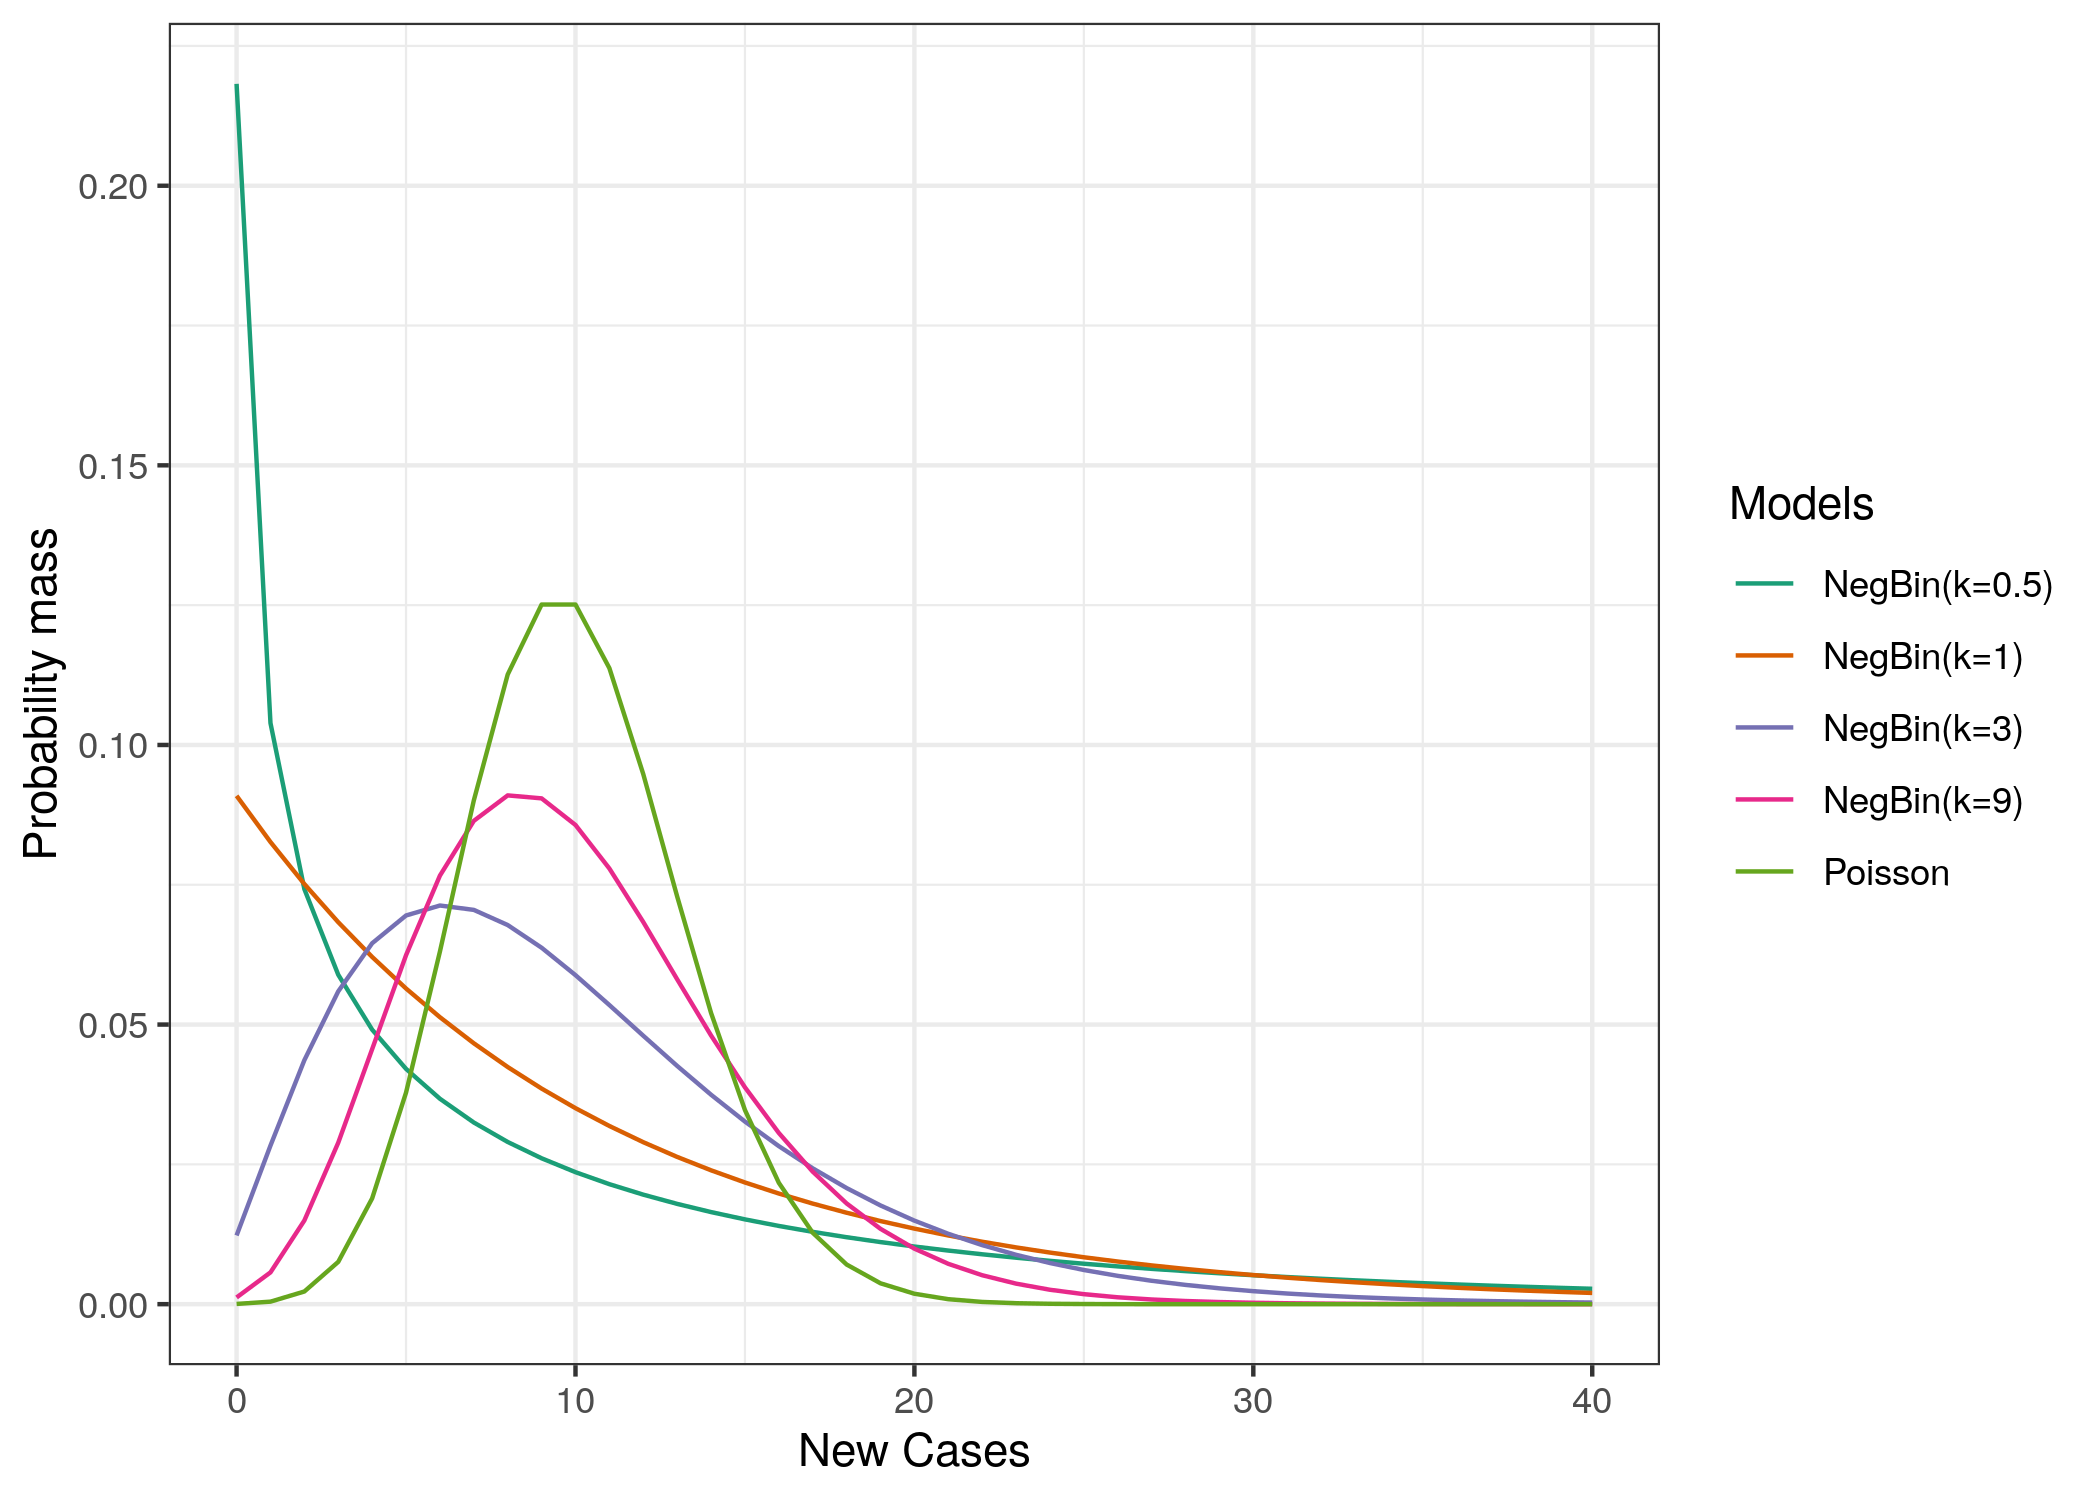
\includegraphics[width=\textwidth]{../output/prob_dist.png}
  \caption{Poisson and negative binomial offspring distributions with a mean of 10.}
  \label{fig:offspring}
\end{figure}

The distribution for $I_t$ would be given by the sum of the offspring distributions for each infected person weighted by the serial distribution. For both the Poisson and negative binomial distribution the sum of independent distributions will give back the same distribution with an expected value given by the sum of the expected values. For the negative binomial distribution the dispersion parameter $k$ will remain the same. 

We will investigate models with offspring distributions based both on the Poisson distribution and the negative binomial distribution to assess which models fit the current outbreak better.

\subsubsection{Reproduction number}
The final ingredient to completely specify the dynamics of the model is the evolution of the reproduction number with time. The function for $R_t$ could be some parametric function where we could fit the parameters to data or we can use non-parametric methods to allow a fairly unconstrained evolution with time. This free function for the reproduction number is what gives the model it's flexibility to fit a large number outbreak types. As for other non-parametric methods we will impose conditions on the rate of change of the reproduction number to reduce the large number of completely unfeasiblefunctions.

%%The model could for example reproduce in expetation a standard compartmental model where the reproduction number is given by $R(t) = R_os(t)$, where $s(t)$ is the fraction of susceptibles. In a normal SIER model with a constant rate to move between the ``E'' and the ``I'' compartment the serial interval woudl be exponential distributed.


In this study we will not use a parametric function for $R_t$, but will instead estimate $R_t$ from the existing data and use these values to predict the future evolution of $R_t$. We will use different methods for forecasting $R_t$ to compare how well they work. 

To estimate the reproduction number from the historical incidence data we use the method developed in \cite{coriNewFrameworkSoftware2013,thompsonImprovedInferenceTimevarying2019}. This approaches used the same formulation as in Equation \ref{eq:mean_It} to estimate the reproduction number from daily incidence and the same serial interval as in our model. If the reproduction number is estimated daily it is likely to vary too much from day to day in a manner that it is unrealistic. Therefore the method averages over the last 7 days to get more stable estimates. A Bayesian procedure is used to estimate both the best fit value and the uncertainty of the estimate. We use the R-package EpiEstim \cite{coriEpiEstimEpiEstimPackage2013} to estimate the reproduction number using a parametric gamma distribution for the serial interval with a mean of 15.3 days and a standard deviation of 9.3 days \cite{whoebolaresponseteamEbolaVirusDisease2014}

Once we have calculated the historical values of $R_t$ we can use them to claculate a forecast for $R_t$ moving forward that can be used for predictions of new incidence. We will use two different procedures to forecast the reproduction number. The first method is a very simple method were we assume that reproduction number remains constant from the last historical value. We use the uncertainties given by the method in \cite{coriNewFrameworkSoftware2013} as a prediction interval. In practice this means that to predict the value of $R_t$ we use the method above to find the parameters of the gamma posterior distribution for $R_{t-1}$. We then get realisations of $R_t$ by drawing random numbers from this posterio distribution. 

The second approach to forecast the reproduction number is based on Bayesian structural time series fitted to the historical values of $R_t$. We use a model with a semi-local linear trend to allow the estimation of a trend in the recent data. To ensure that predicted values of $R_t$ are between 0 and 15 we fit the time series on a transformed scale:

\begin{equation}
r^* = log\left(\frac{R}{15 - R}\right).
\label{eq:transform}
\end{equation}

We use the R-package BSTS \cite{scottBstsBayesianStructural2019} to fit the Bayesian structural time series with the following model:

\[r^*_{t+1} = r^*_t + \delta_t + \epsilon_t, \epsilon_t \sim N(0, \sigma_\mu),\]
\[\delta_{t+1} = D + \phi(\delta_t - D) + \eta_t, \eta_t \sim N(0, \sigma_\delta).\]

$\delta_t$ is the semi-local trend that we model as an AR(1) process that can oscillate around a level $D$. Inverse gamma-priors are used for the standard deviation parameters $\sigma_\mu$ and $\sigma_\delta$, a Gaussian prior on $D$ and a $N(0, 0.1)$ prior for $\phi$. The $\phi$ parameter determines how much the trend behaves as a random-walk. For $\phi=1$ the trend follows a random walk, while for $\phi=0$ the trend is just constant with gaussian noise. We use a prior for small values of $\phi$ to keep the model for having very rapid growth in the variance of $r^*$ that would make the model too over-dispersed. A Markow Chain Monte Carlo (MCMC) algorithm is used to estimate the parameters in the model which then allows us to forecast future values of $r*$. After the model is fitted for all the values up to  $r^*_{t-1}$ we can draw samples of the predictive distribution for $r^*_t$. After using the inverse transform of Equation \ref{eq:transform} to get predictions for $R_t$ we can use these values to forecast incidence. 


\subsubsection{Forecasting incidence}

Once we have specified our model by specifying the offspring distribution and the method for forecasting $R_t$ we can use the model to generate probabilistic forecasts. As in many other application, the forecast is not available in a closed form, but we can simulate the  model to get a sample of values from the predictive distribtion. If we want to generate a forecast for $I_{t+1}$ we first use all the data up until time $t$ to estimate the history of the reproduction number until time $t$. Our probabilistic forecast will be based on sampling possible outcomes to generate a distribution of outcomes. We therefore first draw sample for $R_{t+1}$ from the predictive distributions of the models discussed above, then we combine this with the historical incidence data to calculate the total forece of infection $\lambda_{t+1}$. We then sample $I_{t+1}$ from the specified offspring distribution with an expected value given by $\lambda_{t+1}$. If we want to forecast over multiple time-steps we follow the same procedure by sampling values for the reproduction number. When calculating $\lambda_{t+2}$ we use the sampled value for $I_{t+1}$ together with the historical data ${I_s}$ for $s\leq t$. 


\subsection{Assessing probabilistic forecasts}

The aim of probabilistic forecasts is to predict both the correct average value and the correct probabilities for the different possible outcomes. Therefore, when evaluating such forecasts it is not sufficient to only use metrics that only depend on the point estimate, for example the root mean square error. To assess the forecasts of the models discussed in the previous section we will follow the paradigm of maximising sharpness of the predictive distribution subject to calibration \cite{gneitingProbabilisticForecastsCalibration2007}. In addition we will consider proper scoring rules for comparing probability distributions. We follow the approach taken in \cite{funkAssessingPerformanceRealtime2019}, where probabilistic forecasts for the West African Ebola outbreak were assessed using similar methods.

A model is calibrated if the forecasted distribution is equal to the actual distribution of values. This means that the model can accurately assess it's own uncertainty. For example if we predict that it will rain with a 60\% chance and we find that over time it does rain 60\% of days wheen we predicted a 60\% chance of rain, the model would be well calibrated. Mathematically, if we assume that real distribution of outcomes in nature is given by a cumulative density function $G_t$ and our model predicts a cumulative density function $F_t$, we say that the forecast is ideal and perfectly calibrated if $F_t=G_t$. To assess calibration we will use a randomised Probability Integral Transformation (PIT) \cite{czadoPredictiveModelAssessment2009a}. We consider a forcasted cumulative distribution $F_t$ compared to an observed value $k_t$. For each such pair of forecasts and observed value we calculate:
\[ u_t = F_t(k_t) + \nu (F_t(k_t) - F_t(k_t -1)),\]
where $\nu$ is a standard uniform random variable. If the prediction is ideal, the $u_t$ will be distributed as a standard uniform distribution. Once we have calculated a set of $u_t$ values we can then use the Anderson-Darling test of uniformity (goftest \cite{farawayGoftestClassicalGoodnessofFit2017}) to assess if the distribution of $u_t$ is uniform. If the p-value for this test is less than 0.1 we can reject that the model is calibrated. It is important to note that uniform PIT values is a necessary, but not sufficient condition for an ideal forecast and since we only have limited data that we might not be able to reject calibration even if the model is not well calibrated. In addition to assessing calibration, a histogram of PIT values can tell us if the forecast is under or over-dispersed\cite{czadoPredictiveModelAssessment2009a}. If the forecast is too dispersed the PIT values are likely to cluster in the centre of the PIT histogram, while if the forecast is under-dispersed they are likely to cluster along the edges of th histogram. We use a simple measure of centrality, which is equal to the fraction of $u_t$ values that are between 0.25 and 0.75 as a way to assess if the forecasts are under or over dispersed if they are not calibrated
\[\text{centrality} = \frac{N(0.25 < u_t < 0.75)}{N} - 0.5.\]

When the centrality scores is less than 0, most of the PIT values or outside of central region suggesting that the forecasts are underestimating the real uncertainty.  If the centrality score is larger than 0 then the PIT scores are mainly in the central region and this indicates that the forecasts are overestimating the amount of uncertainty. Since the PIT values include a random component, we will for each set of forecasts repat repeat the calculations of the PIT values 10 times and take averages to average out the effect of the randomness in the definition of $u_t$. 

Sharpness is defined as the range of values in the forecast. The sharper a forecast, the more certain we are of the predicted values. Sharpness depends only on the forecast and not on the observed values. We will use the normalised absolute deviation about the median of y to quantify sharpness:

\[ S_t(F_t) = \frac{1}{0.675} \text{median}(|y - median(y)),\]
the normalisation factor means that $S_t$ is equal to the standard deviation if $F_t$ is normal.

It is also of importance to assess the bias of the forecast. Are we more likely to predict too large or too small values? We will quantity bias as
\[B_t(F_t, k_t) = 1 - (F_t(k_t) - F_t(k_t - 1)).\]
If $B_t=0$ half the probability mass is above and half below the observed value, and the the forecast is unbiased. $B_t$ is between -1 and 1, with both extreme values signifying a completely biased forecast.

Proper scoring rules have been developed to rank forecasts. They combined calibration and sharpness and give a consistent ranking of forecasts. We will use the the continuously ranked probability score (CRPS) and the Dawid-Sebastiani score (DSS) as implemented in the scoringRules package \cite{jordanEvaluatingProbabilisticForecasts2018} for samples from the predictive distribution. The CRPS score is given by 
\[CRPS(F_t,k_t) = \int_R(F_t(z) - \mathds{1}{k_t \leq z})^2 dz,\]
and the DSS only depends on the mean, $\mu_p$ and standard deviation, $\sigma_p$ of the predictive distribution
\[DSS(F_t, k_t) = \left(\frac{k_t- \mu_p}{\sigma_p}\right)^2 + 2\log\sigma_p.\]
The DSS allows an intuitive understanding of the proper scoring rules. The first term tells us about how far away the observed value is from the mean of the predictive distribution in units of the standard deviation and the second term gives information about the sharpness of the predictive distribution. For our models we will only have samples from the predictive distribution. To calculate the CRPS a kernel density estimate is used to estimate $F_t$, for the DSS we use the mean and standard deviation of the sample. 

\subsection{Implementation}
The models were implemented in the R programming language \cite{rcoreteamLanguageEnvironmentStatistical2018} and are available  at http://github.com/gulfa/msc\_ebola. We will consider four different models to assess which model fits the data best. The models are:

\begin{enumerate}
\item{Model 1 (Poisson Latest): Constant reproduction number and Poisson offspring distribution}
\item{Model 2 (NegBin Latest): Constant reproduction number and negative binomial offspring distribution}
\item{Model 3 (Poisson Semi-local): Varying reproduction number and Poisson offspring distribution}
\item{Model 4 (NegBin Semi-local): Varying reproduction number and negative binomial offspring distribution}
\end{enumerate}

For the dispersion parameter $k$ for the negative binomial models we fit a value for the simple negative binomial model by minimising the continuous ranked probability score for the one day ahead predictions for the model on the level of the whole outbreak. 

We will assess how well the models work both for the entire epidemic and for each health zone. To evaluate a model we will estimate the calibration, sharpness, bias, log score and CRPS for forecasts up to 28 days ahead. To do this we start 17 days\footnote{The 17 days are due the fact that method for estimating the reproduction number needs thi smany days to give reasonable values for the reproduction number} after the first case of the epidemic in the location and calculate the $d$-ahead prediction for all historically available data. For the calibration we use all forecasts for the $d$-ahead compared to the observed values the values to assess if PIT values are uniformly distributed, while for all the other metrics we average them over all the time steps.



\section{Results}

From the start of the 2018--2019 DRC Ebola outbreak until the 31st of August 2019 there has been 2,926 confirmed Ebola cases and 1926 confirmed Ebola deaths. This gives a high Case Fatality Ratio of 66\%. Figure \ref{fig:epi_curve} shows the weekly number of cases and the map in Figure \ref{fig:tot_map} the total number of cases from each Health Zone. From Figure \ref{fig:epi_curve} and the estimate of the instantaneous reproduction number in Figure \ref{fig:rep_num} we can see the evolution of the outbreak. After the initial period with varrying weekly case numbers, there was an increase in cases from October 2018 with a large reproduction number, followed by a more varied period where the reproduction number varied around 1 with some waves of larger reproduction number. From March 2019 the number of cases per week increased significantly, with a continuing large number of cases in June and July even if the reproduction number decreased. From July 2019 the reproduction has varied around one, indicating that the outbreak is still not under control, but that the intensity of the outbreak is less than in May and June. From the epi-curve there seems to be some connection between large increases in incidence and introduction or reintroduction into specific health zones. We can also see that the disease is moving around between health zones where at different time the incidences is dominated by different health zones. 

\begin{figure}[h!]
\begin{subfigure}{0.48\textwidth}
  \centering

  % include first image
  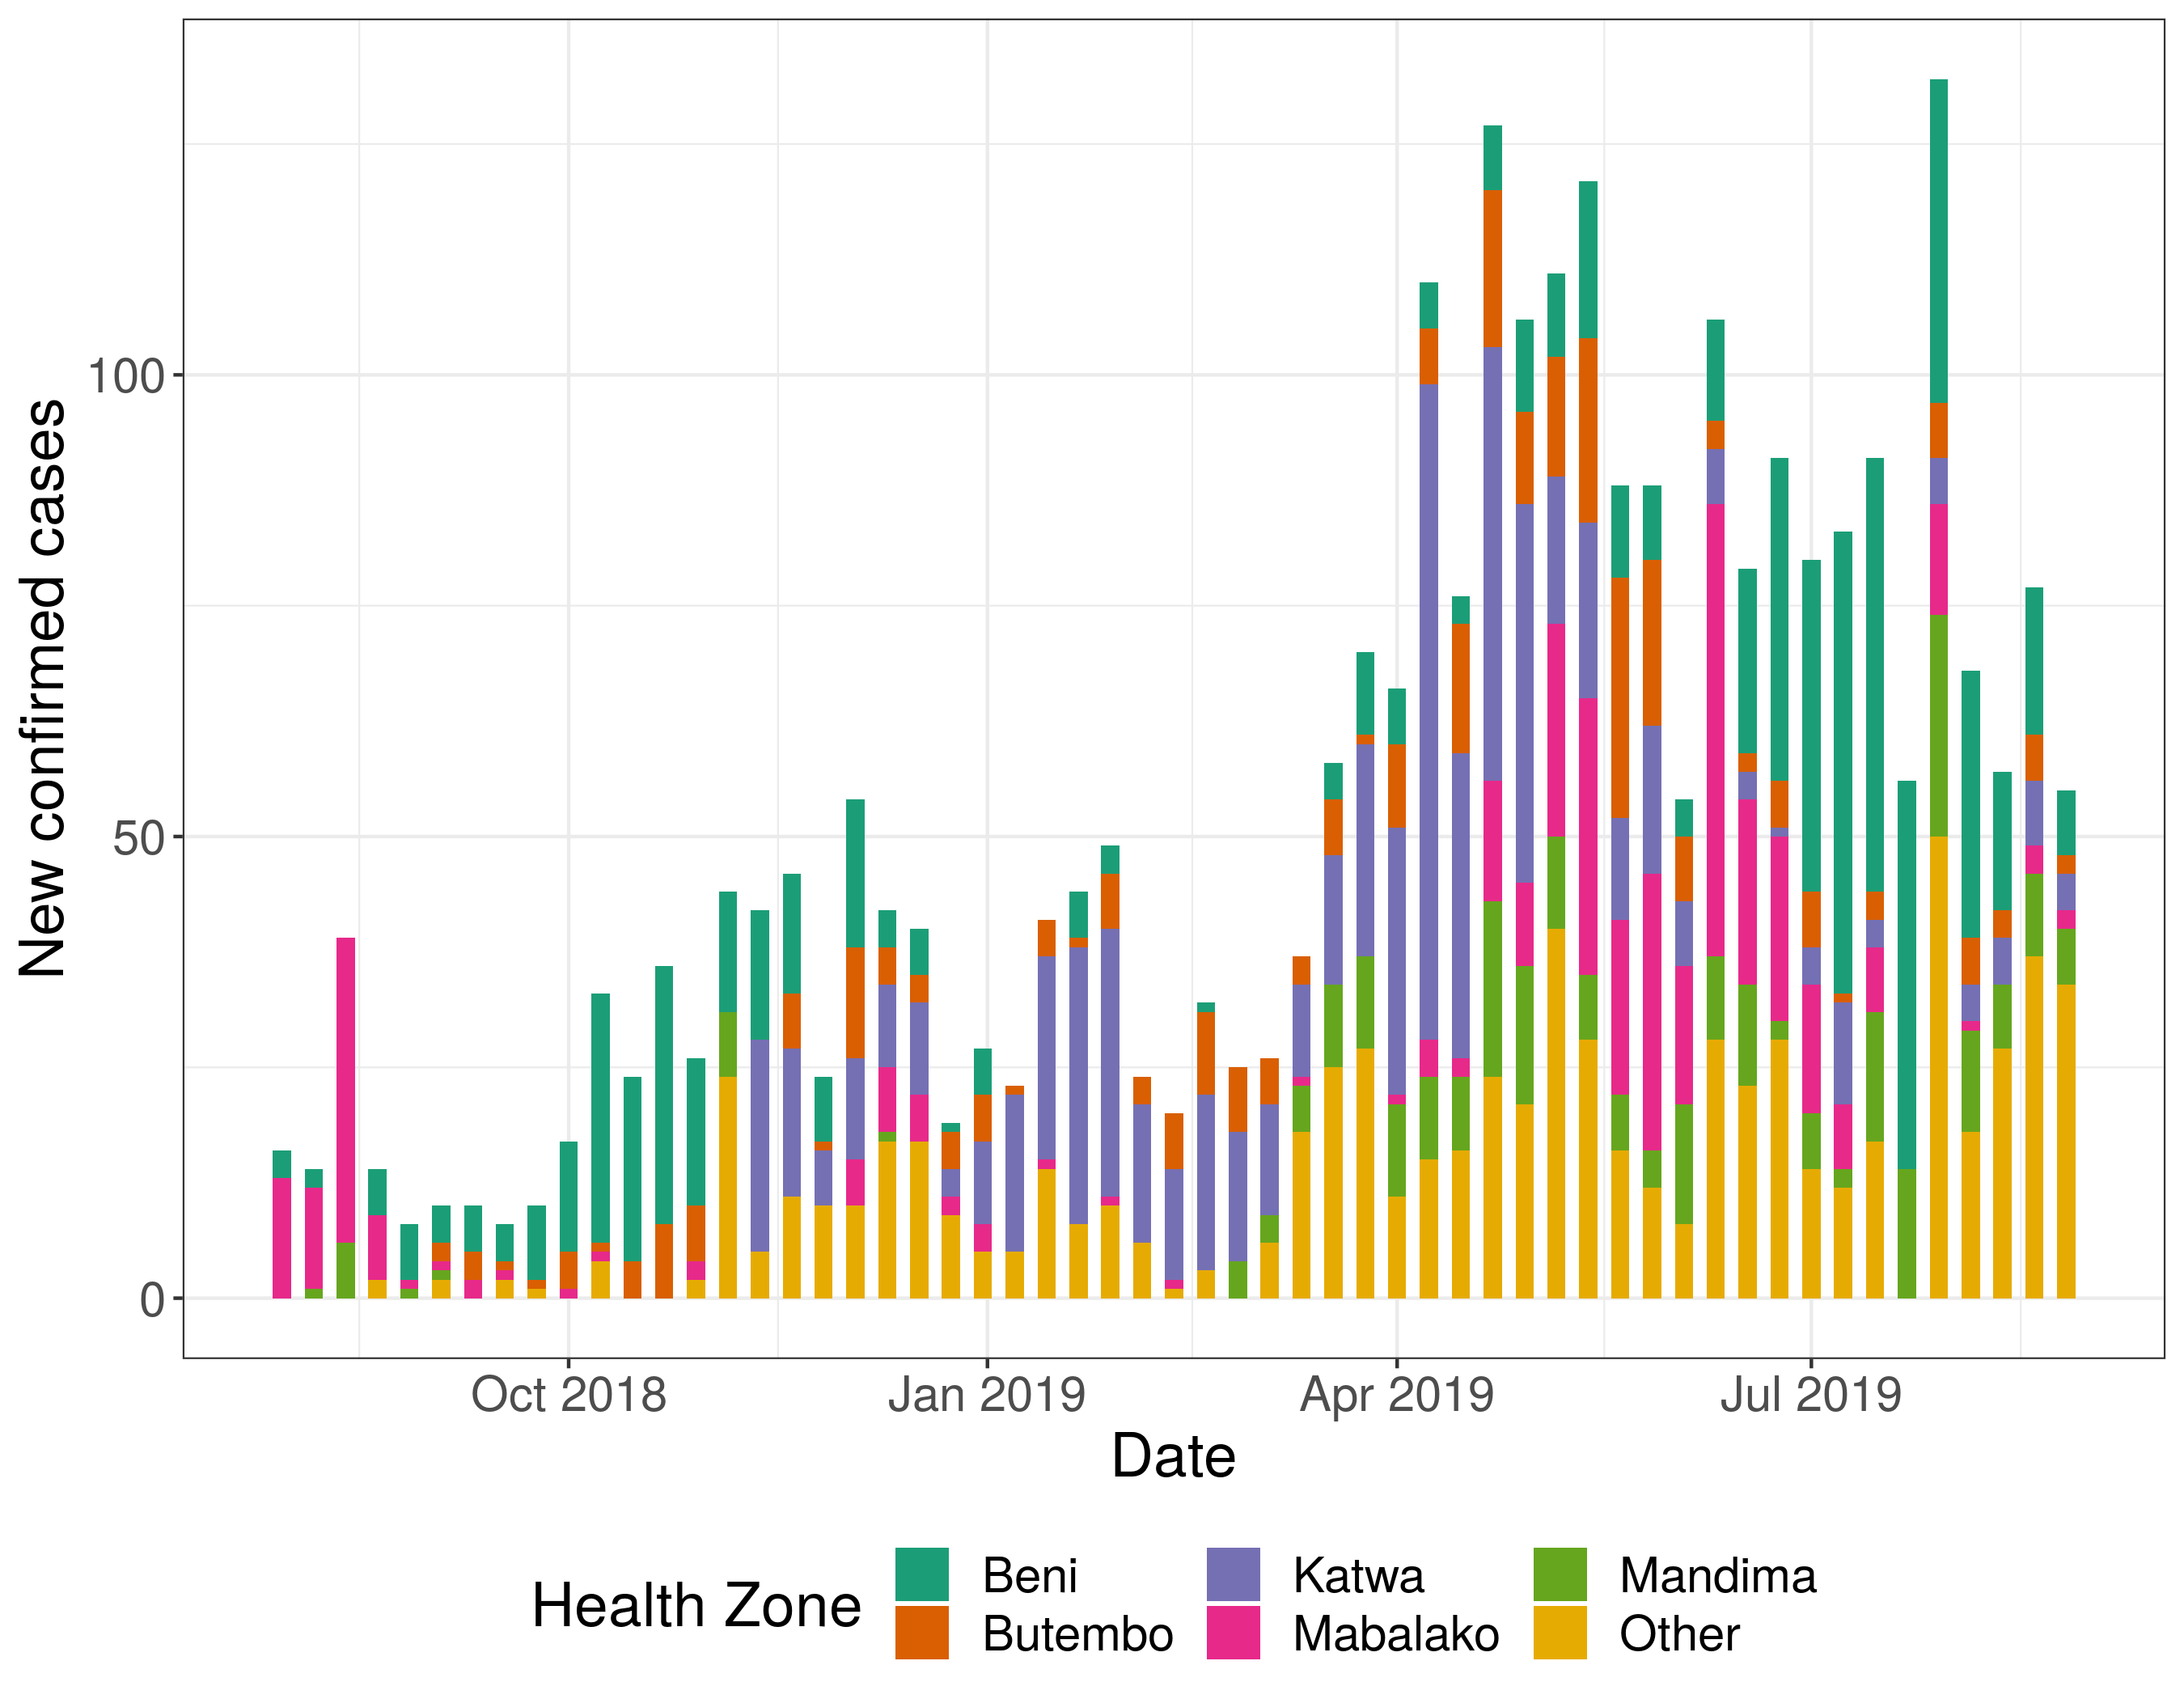
\includegraphics[width=\textwidth]{../output/epi_curve.png}
  \caption{Number of new confirmed cases by week in the health zones with the most Ebola Cases}
  \label{fig:epi_curve}
\end{subfigure}
\begin{subfigure}{0.48\textwidth}
  \centering
  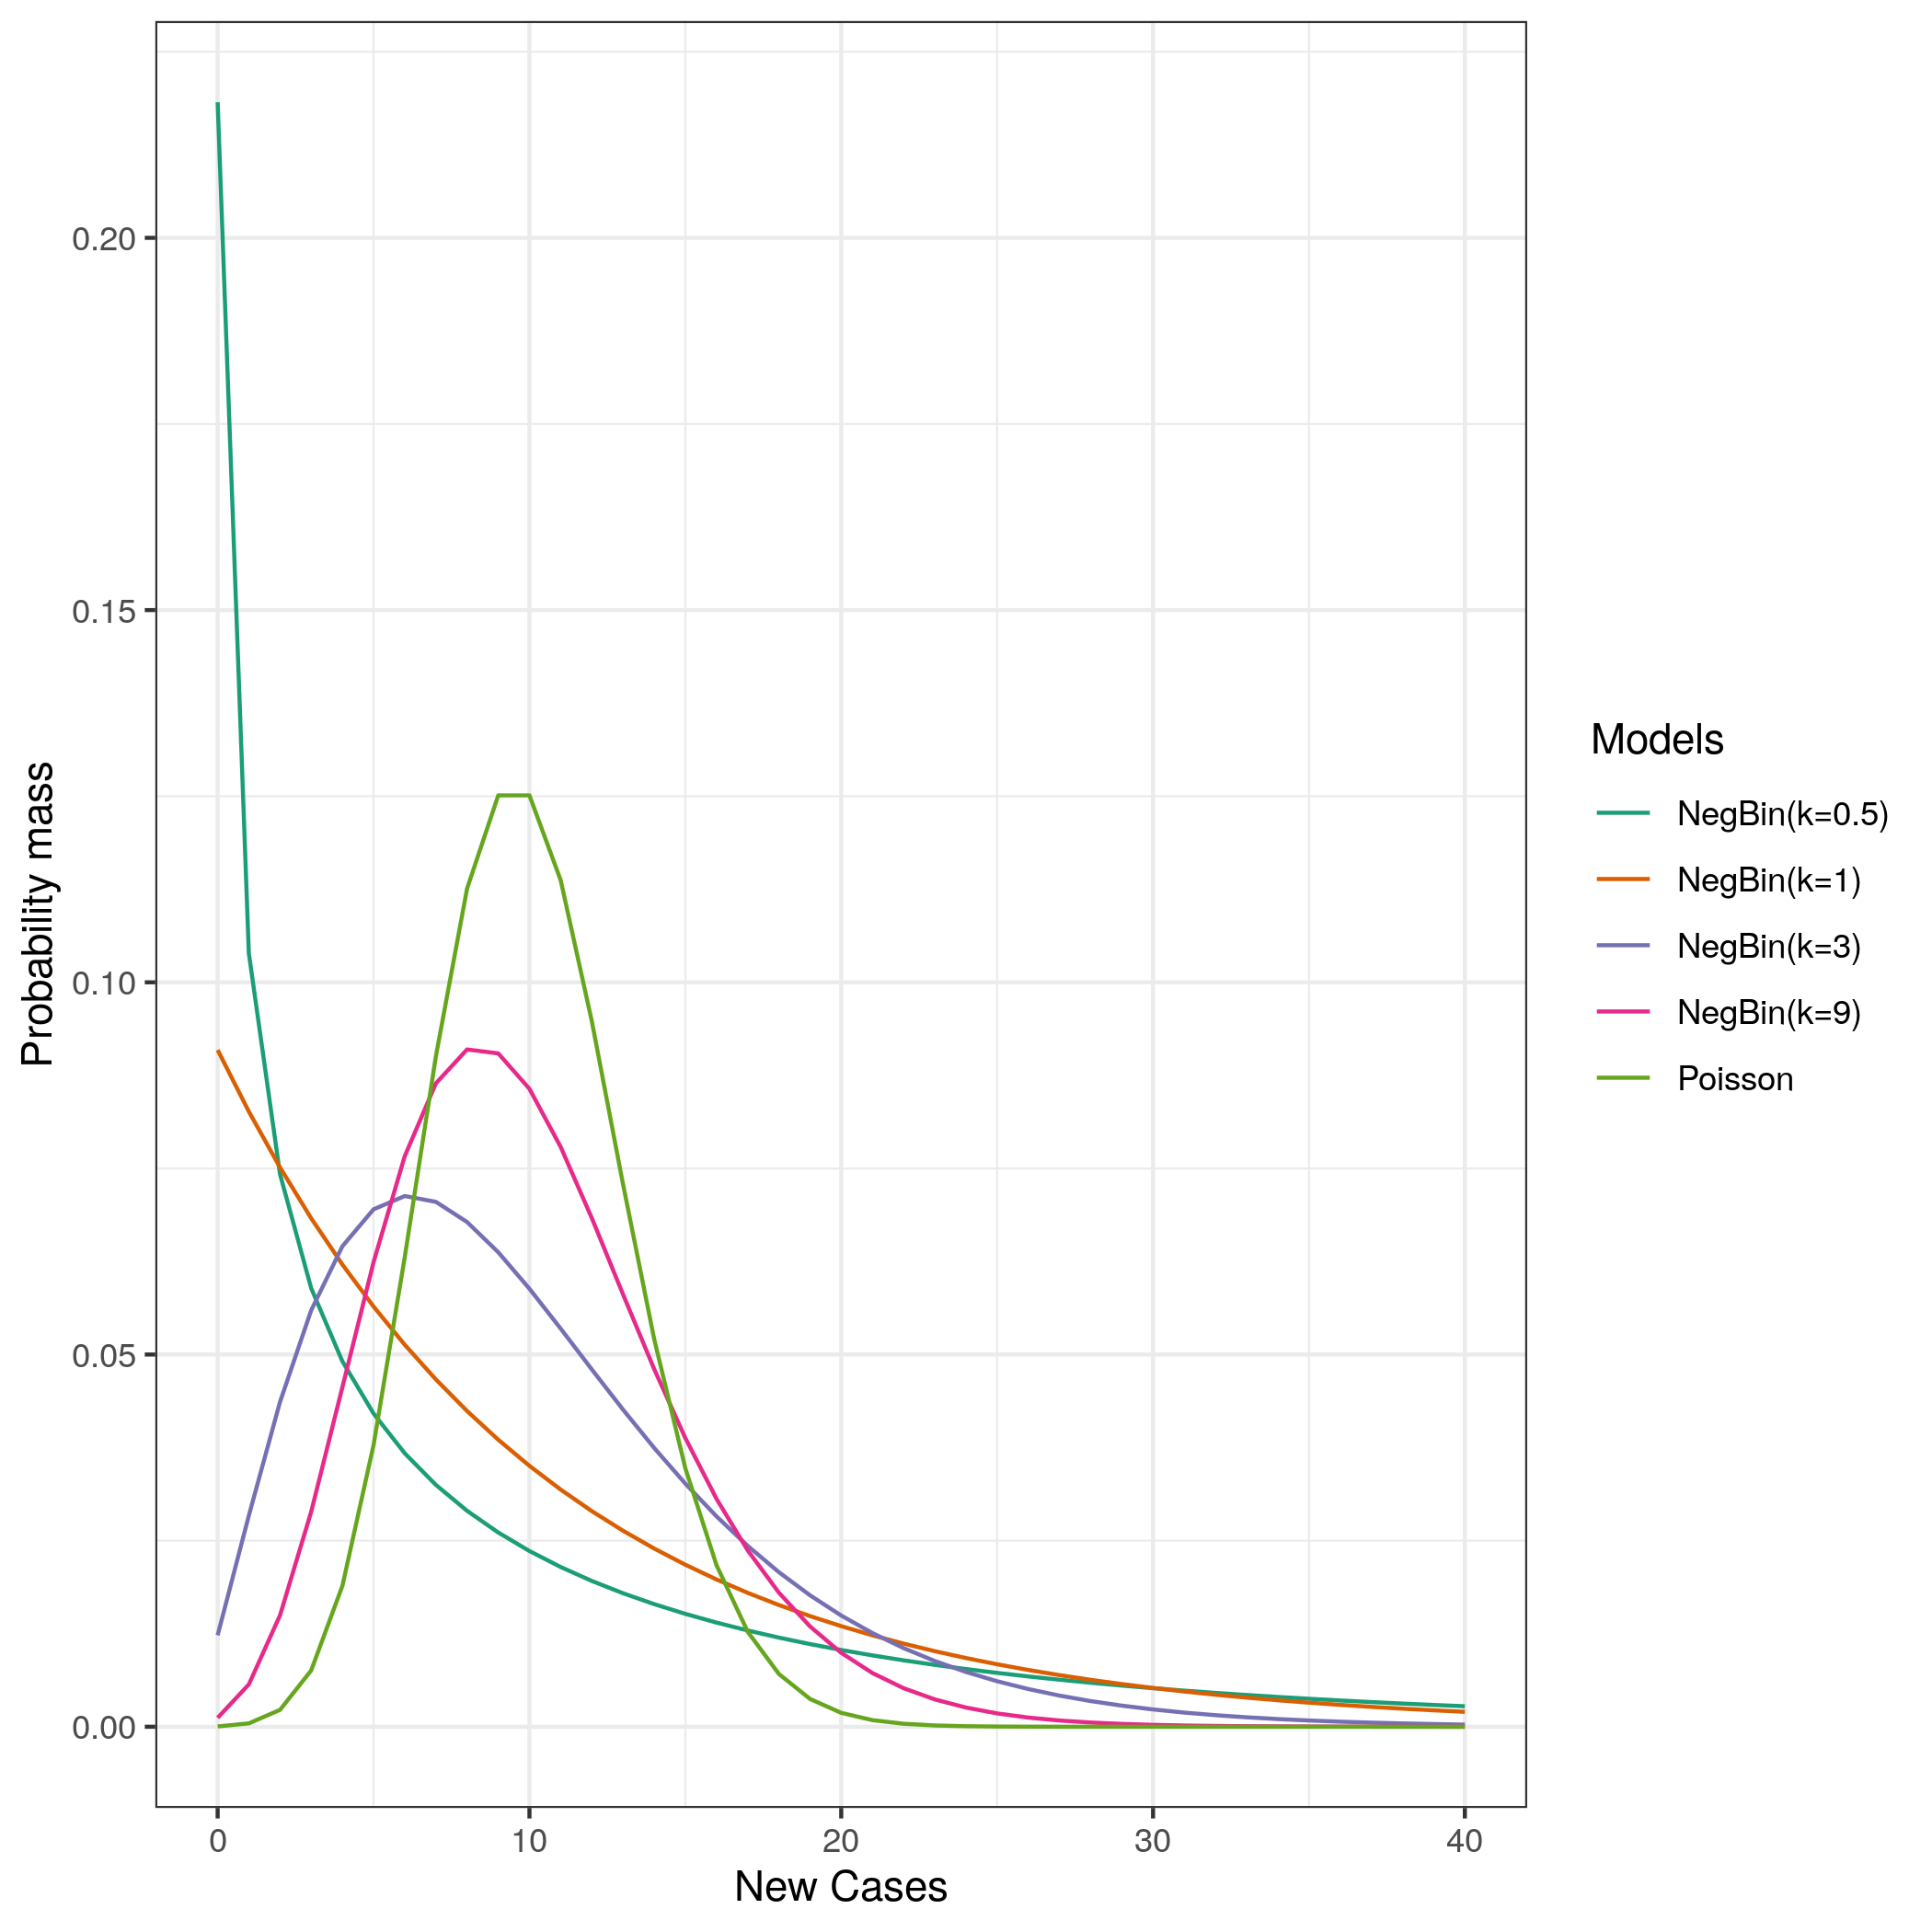
\includegraphics[width=\textwidth]{../output/tot_map.png}
  \caption{Total number of confirmed cases by Health Zone}
  \label{fig:tot_map}
\end{subfigure}

\bigskip

\begin{subfigure}{\textwidth}
  \centering
  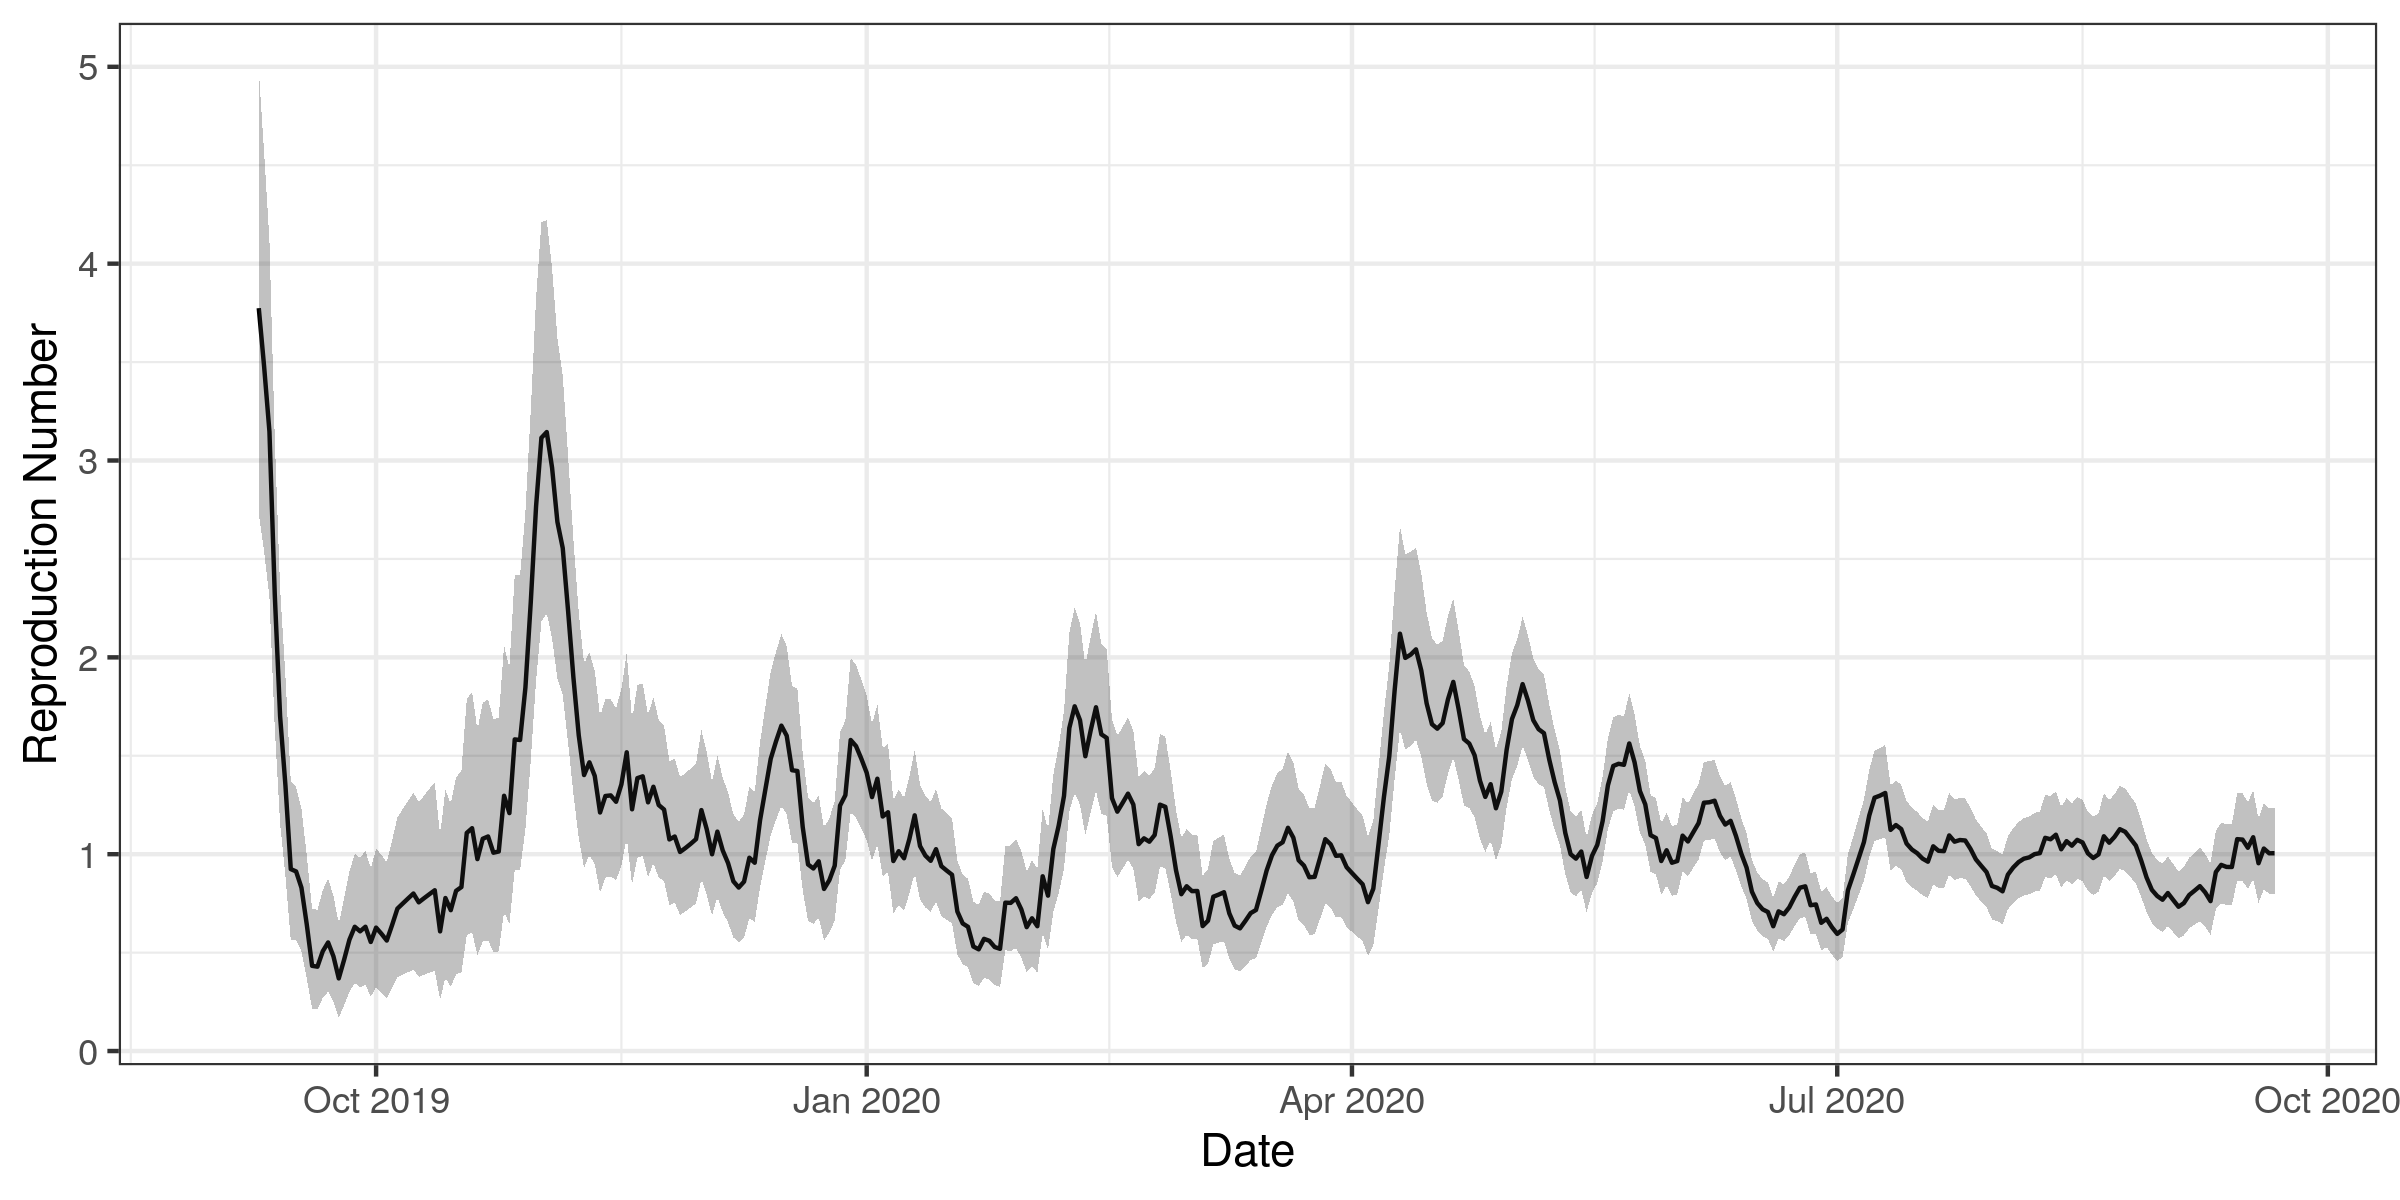
\includegraphics[width=\textwidth]{../output/nat_Rs.png}
  \caption{Reproduction number as a function of time, the shaded region shows the 95\% credible interval}
  \label{fig:rep_num}
\end{subfigure}
\end{figure}

\subsection{National level forecasts}
The first step in modelling the outbreak on the national level was to find the best fitting value of the dispersion parameter for the negative binomial models. We found that the dispersion parameter that gives the smallest CRPS score for one day ahead predictions for the negative binomial models was $k\approx8$, but a fairly large range of parameters gave a reasonable fit. We therefore chose to use $k=8$ for the negative binomial distributions both for the national and health zone forecasts.

All four models were successfully fitted on incidence data from 395 days and then used to provide short term forecasts. The calibration and proper scoring rules scores for the four models for different forecasting horizons can be seen in Table \ref{tab:nat_evo} for weekly Forecasting horizons up to four weeks. We also show the the evolution of calibration, bias, CRPS and the centrality of PIT values as a function of the forecasting horizon in Figure \ref{fig:nat_scores}
% latex table generated in R 3.6.1 by xtable 1.8-4 package
<<<<<<< HEAD
% Sat Sep  7 08:33:09 2019
=======
% Tue Sep 10 13:43:43 2019
>>>>>>> 6c96552641a3c339d41f2f58414064ece613e460
\begin{table}[ht]
\centering
\begin{tabular}{rlrrrrrrr}
  \hline
 & model & horizon & sharpness & bias & crps & dss & centrality & calibration \\ 
  \hline
<<<<<<< HEAD
1 & Negative Binomial Semilocal &   1 & 4.08 & -0.03 & 1.87 & 3.30 & 0.55 & 0.19 \\ 
  2 & Negative Binomial Latest &   1 & 4.14 & -0.00 & 1.82 & 3.26 & 0.56 & 0.17 \\ 
  3 & Poisson Semilocal &   1 & 2.93 & 0.01 & 1.87 & 3.32 & 0.43 & 0.00 \\ 
  4 & Poisson Latest &   1 & 2.97 & 0.05 & 1.82 & 3.24 & 0.42 & 0.00 \\ 
  5 & Negative Binomial Semilocal &   7 & 4.83 & -0.07 & 1.80 & 3.41 & 0.66 & 0.00 \\ 
  6 & Negative Binomial Latest &   7 & 4.33 & 0.01 & 2.36 & 3.94 & 0.47 & 0.00 \\ 
  7 & Poisson Semilocal &   7 & 4.19 & -0.02 & 1.72 & 3.23 & 0.59 & 0.01 \\ 
  8 & Poisson Latest &   7 & 3.08 & 0.06 & 2.47 & 4.31 & 0.36 & 0.00 \\ 
  9 & Negative Binomial Semilocal &  14 & 5.98 & -0.10 & 2.56 & 4.62 & 0.63 & 0.00 \\ 
  10 & Negative Binomial Latest &  14 & 4.62 & 0.02 & 2.82 & 4.74 & 0.41 & 0.00 \\ 
  11 & Poisson Semilocal &  14 & 5.78 & -0.06 & 2.52 & 4.54 & 0.60 & 0.00 \\ 
  12 & Poisson Latest &  14 & 3.28 & 0.09 & 2.99 & 5.32 & 0.29 & 0.00 \\ 
  13 & Negative Binomial Semilocal &  21 & 7.55 & -0.13 & 3.24 & 5.69 & 0.65 & 0.00 \\ 
  14 & Negative Binomial Latest &  21 & 5.12 & 0.01 & 4.07 & 5.57 & 0.31 & 0.00 \\ 
  15 & Poisson Semilocal &  21 & 7.67 & -0.10 & 3.26 & 5.88 & 0.65 & 0.00 \\ 
  16 & Poisson Latest &  21 & 3.53 & 0.06 & 4.54 & 6.85 & 0.24 & 0.00 \\ 
  17 & Negative Binomial Semilocal &  28 & 9.14 & -0.16 & 4.77 & 7.43 & 0.67 & 0.00 \\ 
  18 & Negative Binomial Latest &  28 & 5.87 & 0.03 & 5.30 & 7.38 & 0.30 & 0.00 \\ 
  19 & Poisson Semilocal &  28 & 9.64 & -0.13 & 4.89 & 7.12 & 0.66 & 0.00 \\ 
  20 & Poisson Latest &  28 & 3.88 & 0.08 & 6.00 & 9.08 & 0.22 & 0.00 \\ 
=======
1 & Negative Binomial Semilocal &   1 & 4.08 & -0.65 & 1.87 & 3.30 & 0.05 & 0.19 \\ 
  2 & Negative Binomial Latest &   1 & 4.14 & -0.65 & 1.82 & 3.26 & 0.06 & 0.16 \\ 
  3 & Poisson Semilocal &   1 & 2.93 & -0.65 & 1.87 & 3.32 & -0.07 & 0.00 \\ 
  4 & Poisson Latest &   1 & 2.97 & -0.65 & 1.82 & 3.24 & -0.08 & 0.00 \\ 
  5 & Negative Binomial Semilocal &   7 & 4.83 & -0.65 & 1.80 & 3.41 & 0.16 & 0.00 \\ 
  6 & Negative Binomial Latest &   7 & 4.33 & -0.65 & 2.36 & 3.94 & -0.04 & 0.00 \\ 
  7 & Poisson Semilocal &   7 & 4.19 & -0.65 & 1.72 & 3.23 & 0.09 & 0.01 \\ 
  8 & Poisson Latest &   7 & 3.08 & -0.65 & 2.47 & 4.31 & -0.14 & 0.00 \\ 
  9 & Negative Binomial Semilocal &  14 & 5.98 & -0.66 & 2.56 & 4.62 & 0.14 & 0.00 \\ 
  10 & Negative Binomial Latest &  14 & 4.62 & -0.66 & 2.82 & 4.74 & -0.08 & 0.00 \\ 
  11 & Poisson Semilocal &  14 & 5.78 & -0.66 & 2.52 & 4.54 & 0.10 & 0.00 \\ 
  12 & Poisson Latest &  14 & 3.28 & -0.66 & 2.99 & 5.32 & -0.21 & 0.00 \\ 
  13 & Negative Binomial Semilocal &  21 & 7.55 & -0.67 & 3.24 & 5.69 & 0.15 & 0.00 \\ 
  14 & Negative Binomial Latest &  21 & 5.12 & -0.67 & 4.07 & 5.57 & -0.19 & 0.00 \\ 
  15 & Poisson Semilocal &  21 & 7.67 & -0.67 & 3.26 & 5.88 & 0.16 & 0.00 \\ 
  16 & Poisson Latest &  21 & 3.53 & -0.67 & 4.54 & 6.85 & -0.26 & 0.00 \\ 
  17 & Negative Binomial Semilocal &  28 & 9.14 & -0.68 & 4.77 & 7.43 & 0.17 & 0.00 \\ 
  18 & Negative Binomial Latest &  28 & 5.87 & -0.68 & 5.30 & 7.38 & -0.20 & 0.00 \\ 
  19 & Poisson Semilocal &  28 & 9.64 & -0.68 & 4.89 & 7.12 & 0.16 & 0.00 \\ 
  20 & Poisson Latest &  28 & 3.88 & -0.68 & 6.00 & 9.08 & -0.28 & 0.00 \\ 
>>>>>>> 6c96552641a3c339d41f2f58414064ece613e460
   \hline
\end{tabular}
\caption{Model evaluations for predictions when all the models are fitted on the combined data from all the health zones.} 
\label{tab:nat_evo}
\end{table}



\begin{figure}[h!]
\begin{subfigure}{0.5\textwidth}
  \centering
  % include first image
  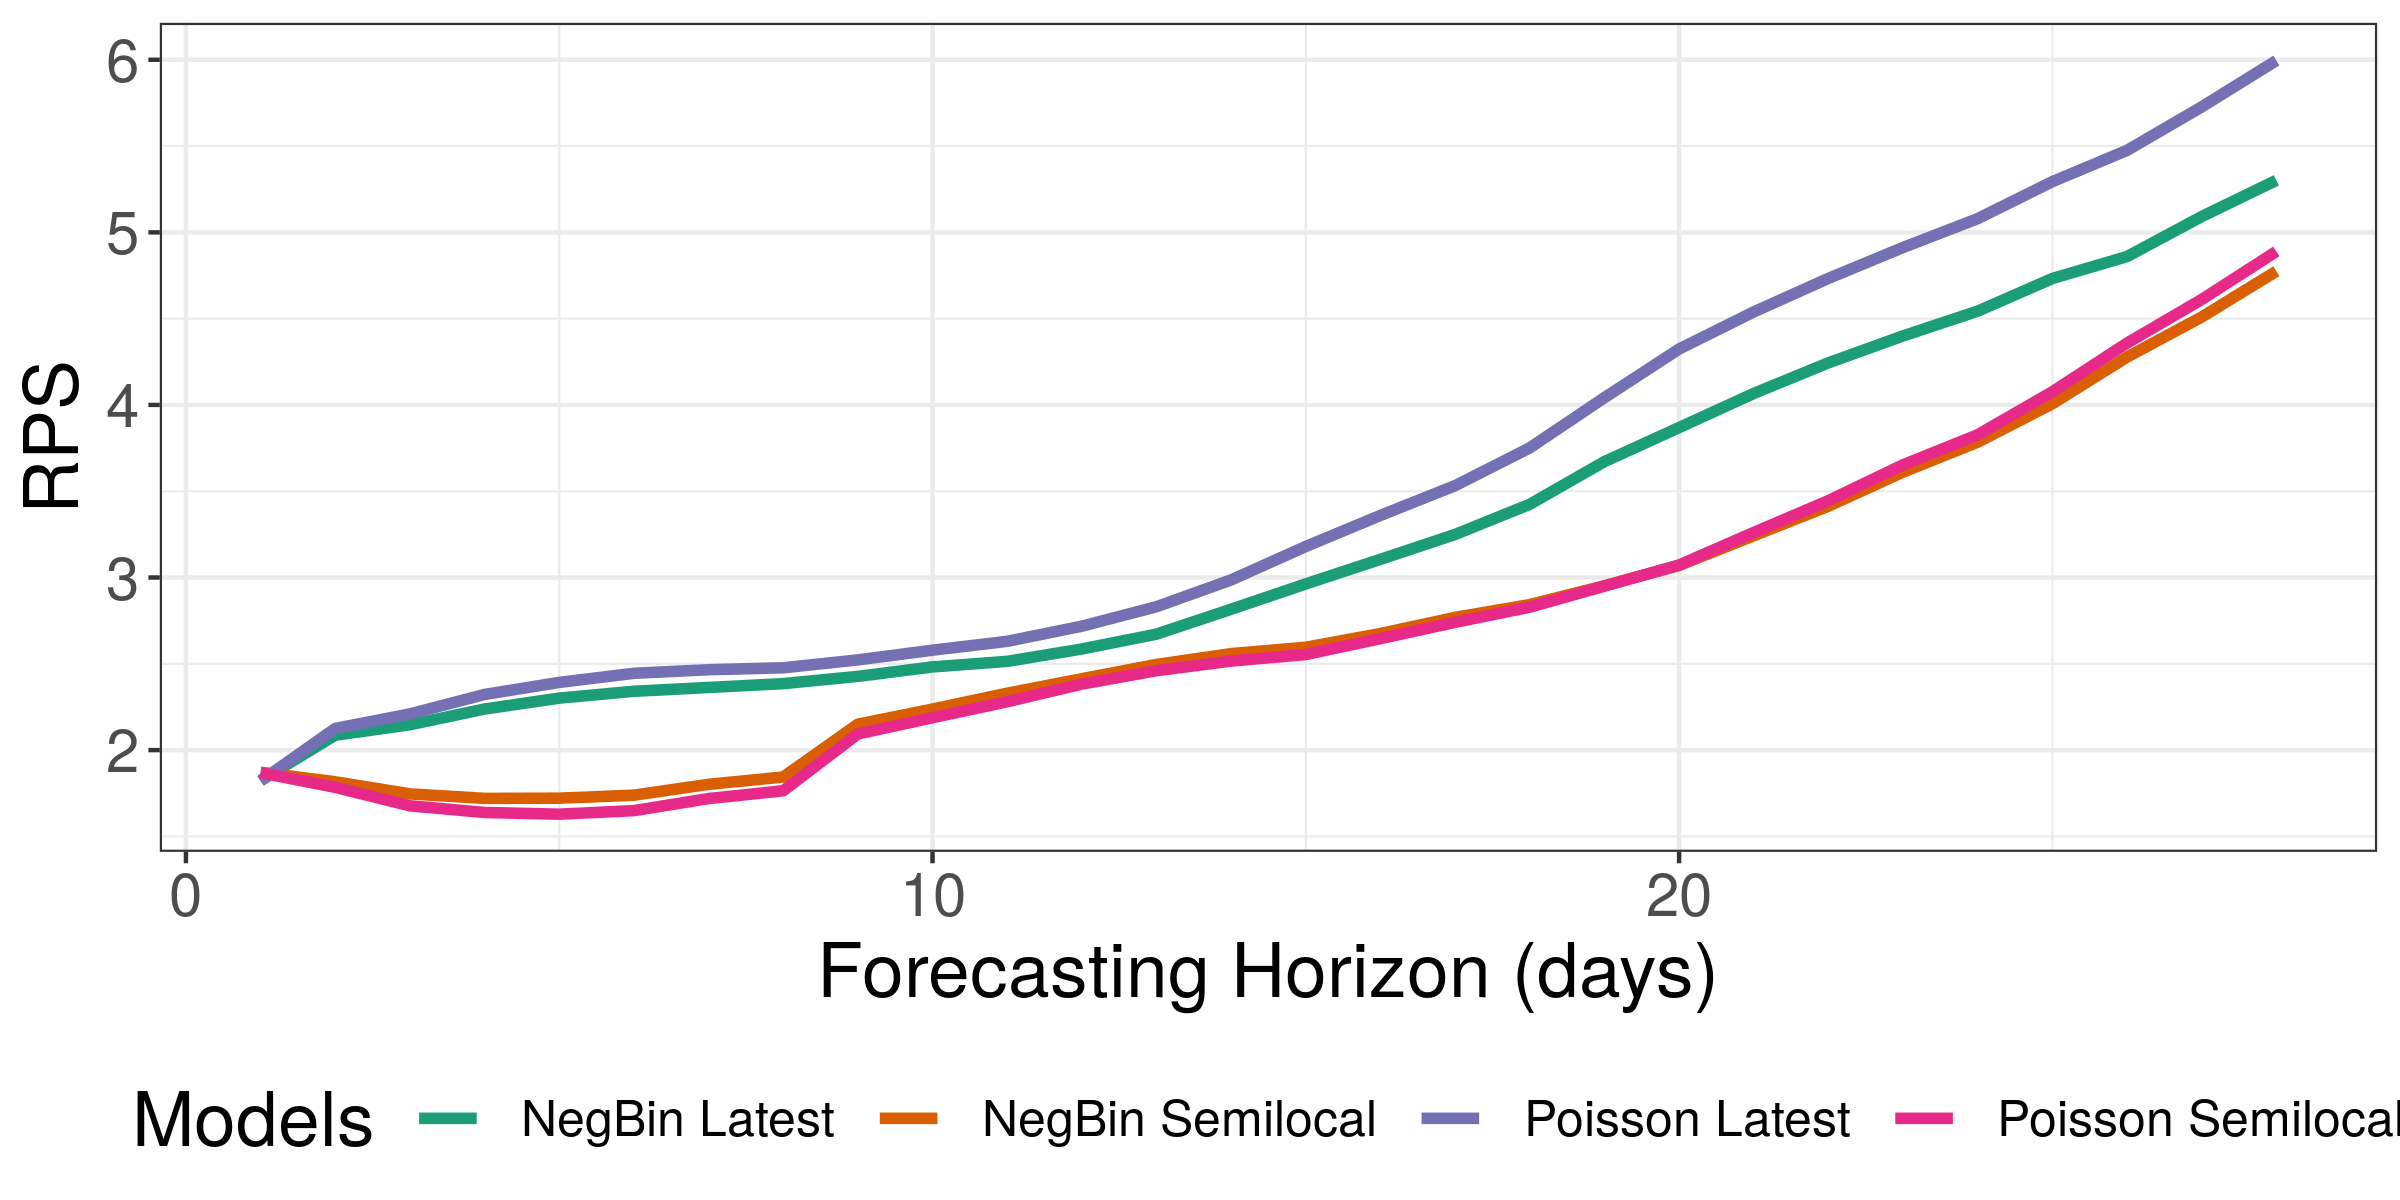
\includegraphics[width=\linewidth]{../output/national_crps.png}  
  \caption{Continuously Ranked Probability Score}
  \label{fig:sub-first}
\end{subfigure}
\begin{subfigure}{0.5\textwidth}
  \centering
  % include second image
  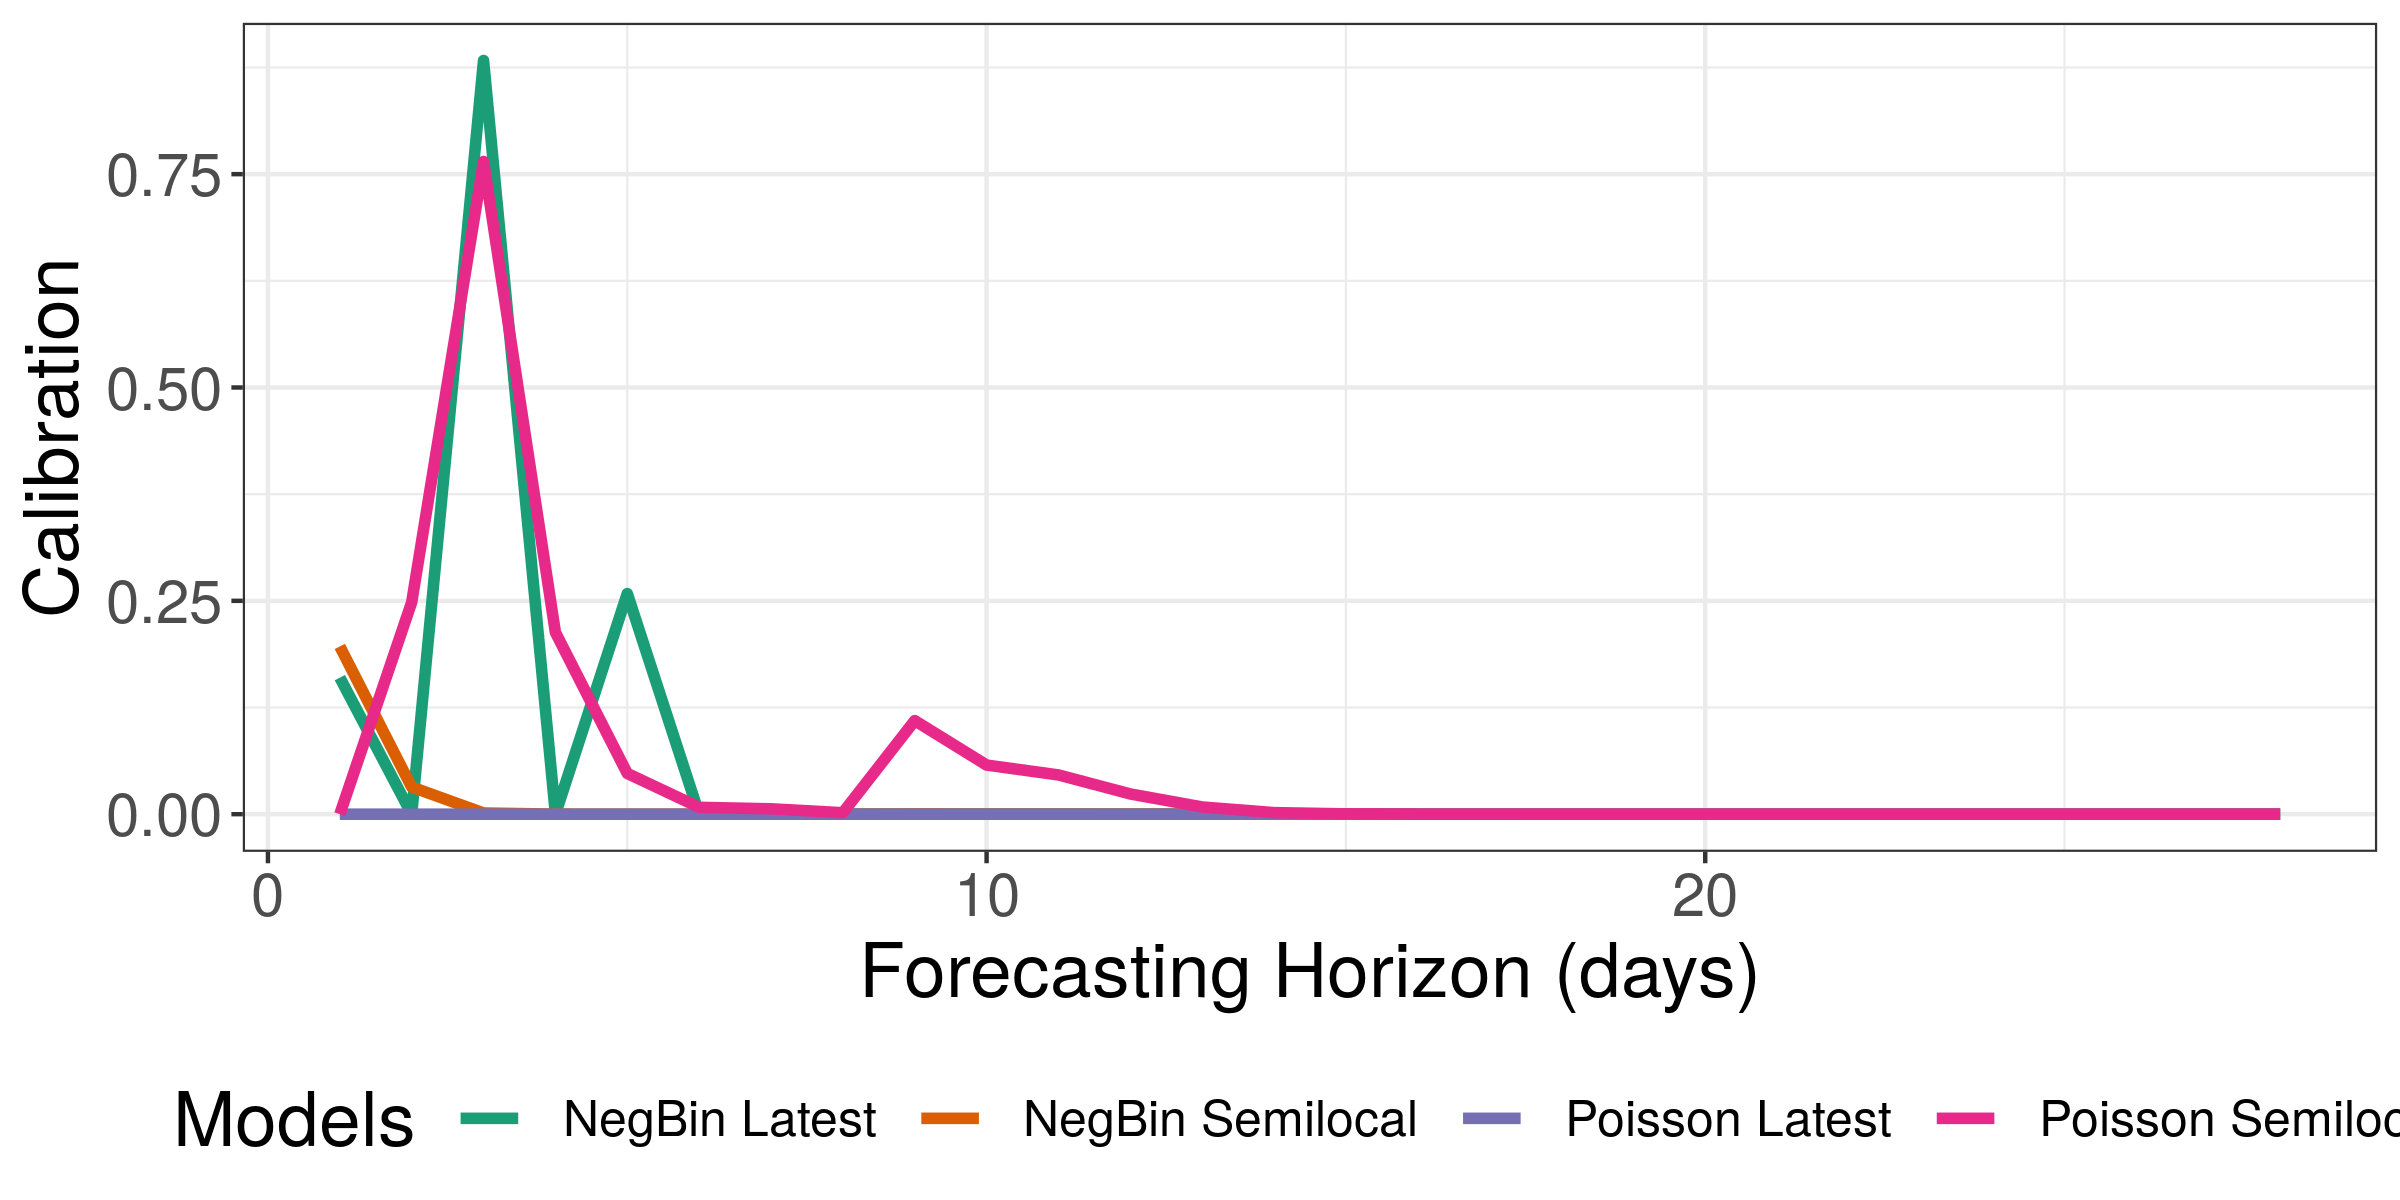
\includegraphics[width=\linewidth]{../output/national_calibration.png}  
  \caption{P-value for calibration of PIT values}
  \label{fig:sub-second}
\end{subfigure}

\begin{subfigure}{0.5\textwidth}
  \centering
  % include second image
  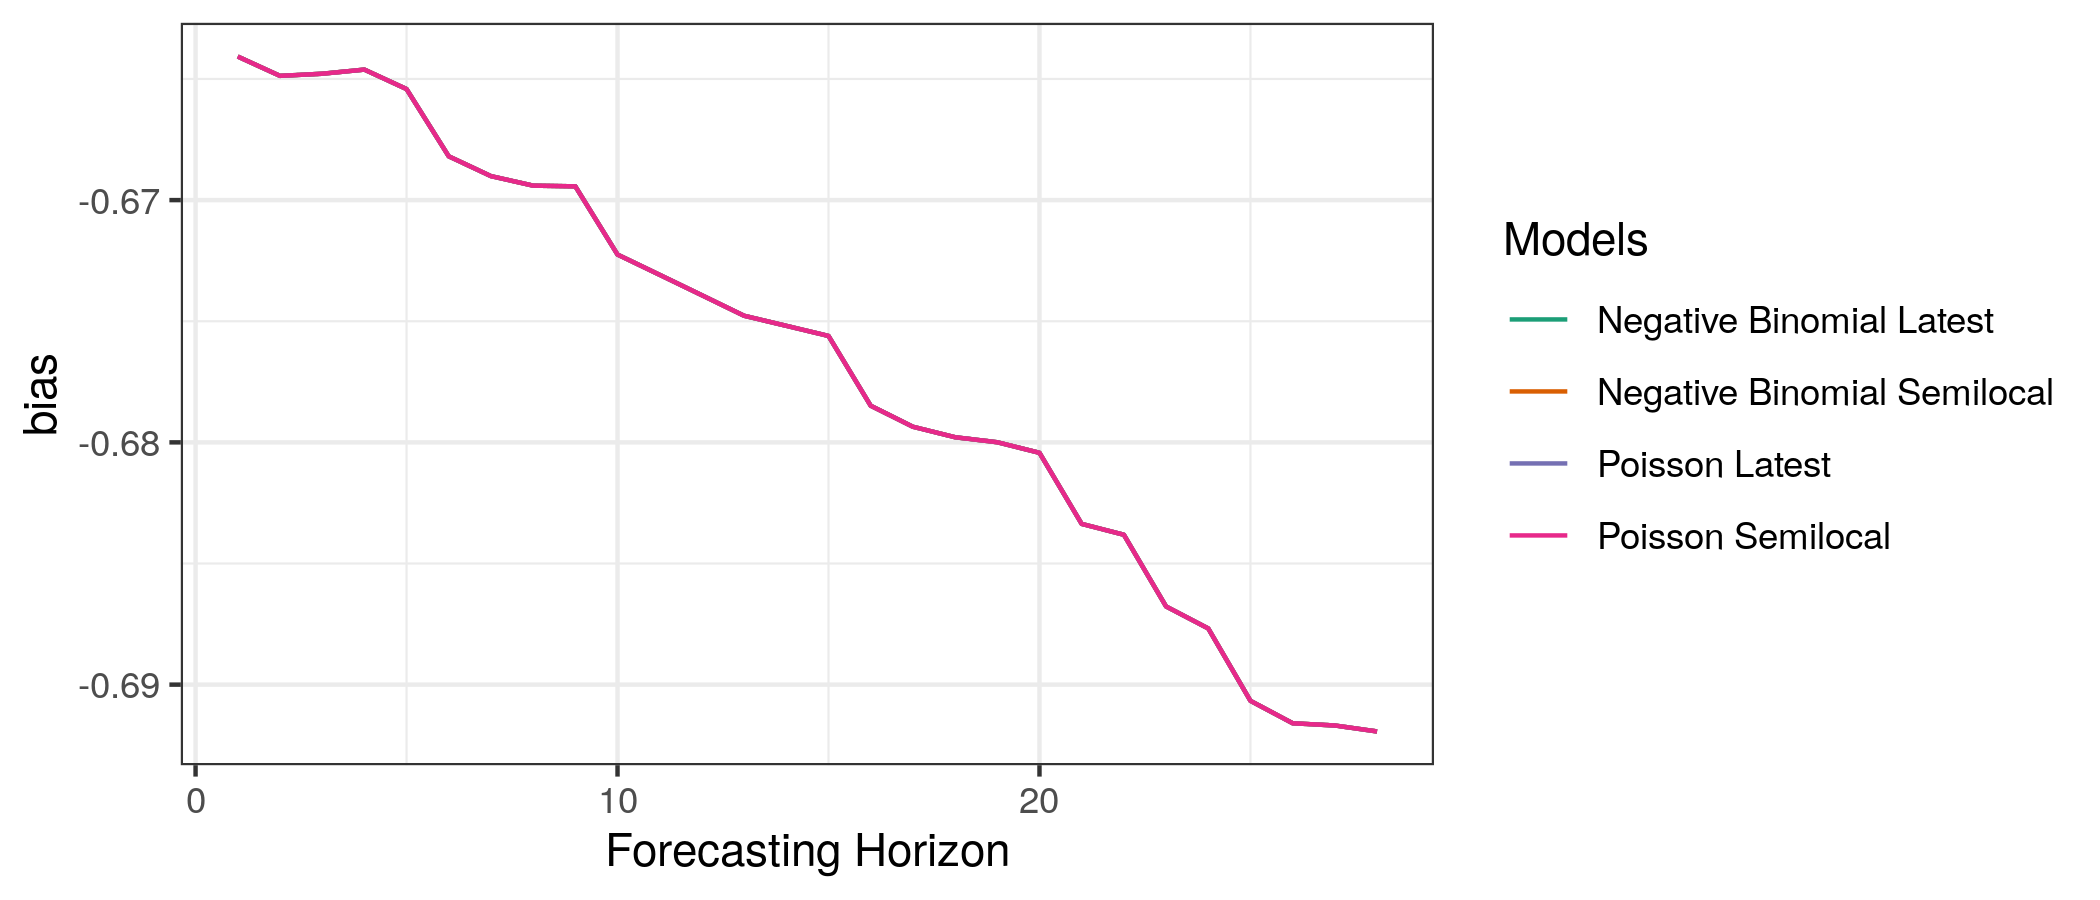
\includegraphics[width=\linewidth]{../output/national_bias.png}  
  \caption{Bias}
  \label{fig:sub-third}
\end{subfigure}
\begin{subfigure}{0.5\textwidth}
  \centering
  % include second image
  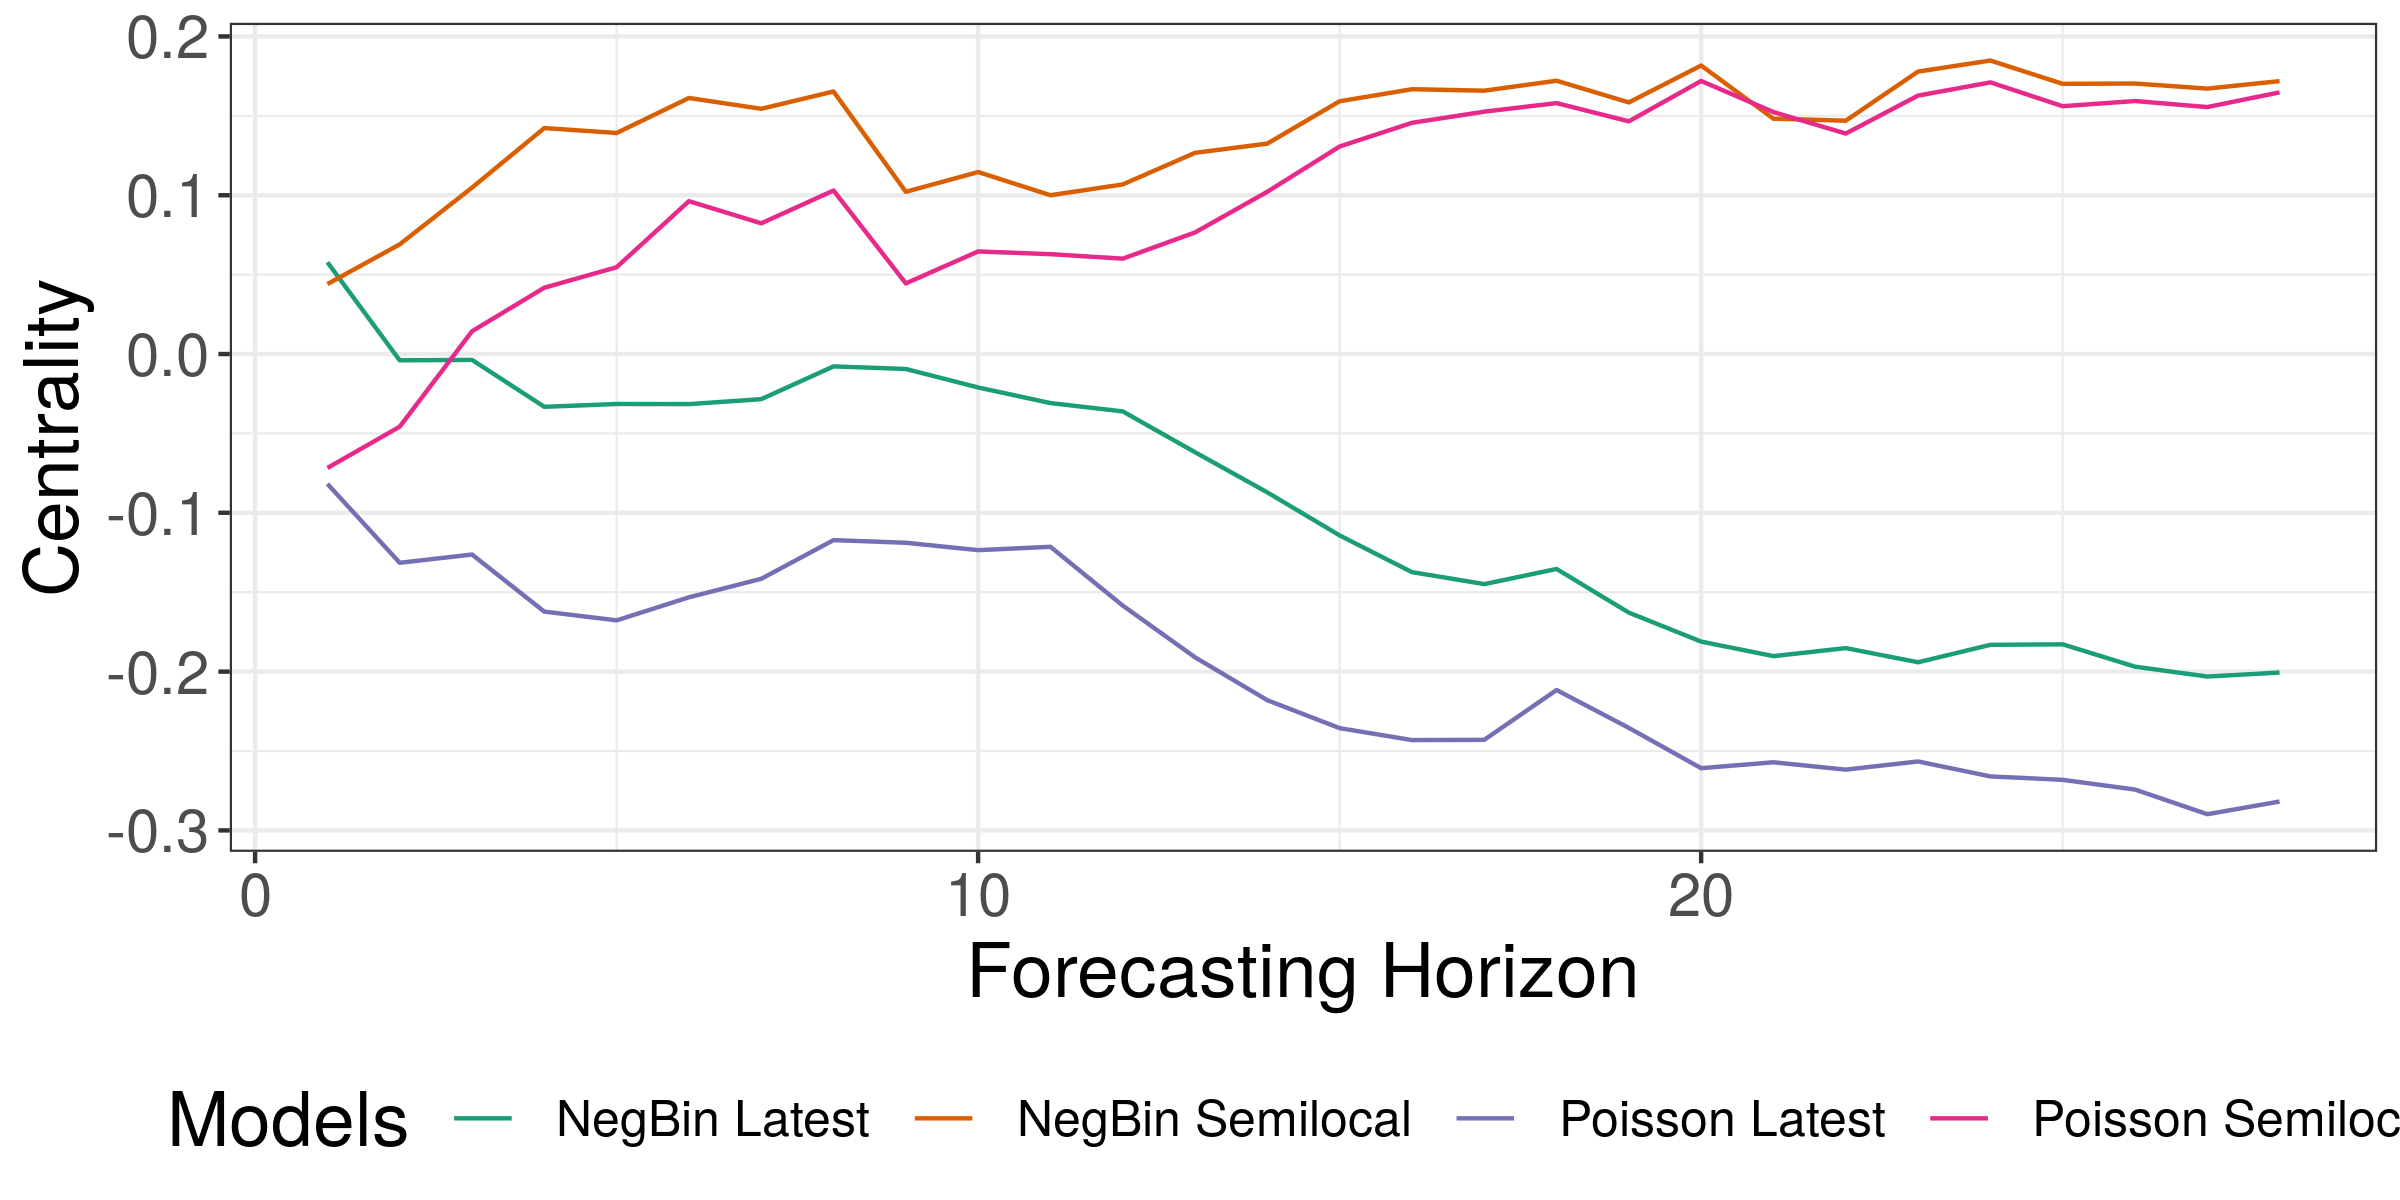
\includegraphics[width=\linewidth]{../output/national_centrality.png}  
  \caption{Centrality of PIT values}
  \label{fig:nat_scores_4}
\end{subfigure}
  \caption{Evaluation of the four models as a function of forecasting horizon for the whole outbreak}

  \label{fig:nat_scores}
\end{figure}

Together they show that for next day forecast, the negative binomial offspring distribution is needed for a calibrated forecast as only the two negative binomial models are calibrated with a p-value larger than 0.1. We can also see that there are no big differences for one-day ahead forecasts based on the method of forecasting the reproduction number. For longer forecasting horizons the Poisson distribution with the semi-local time series prediction for $R_t$ is the best model and is calibrated up until 9 days. This is the only model that is calibrated for longer forecasting horizons and it also has the lowest CRPS and DSS scores. The centrality of the PIT scores in Figure \ref{fig:nat_scores_4} give us extra information about how our models fail. A negative centrality means that the model has too little uncertainty and we can see that this is the case for the two models based on using the latest reproduction number. The two models using the semi-local trend for the reproduction number are closer to zero centrality, but they have too much uncertainty since their centrality score is above zero. For the same method of forecasting the reproduction number, the negative binomial models always have larger uncertainty as we can also see from the sharpness figures. And as after about one week the sharpness of the poisson semilocal model has grown to be the same as the negative binomial latest model. We can see how the semilocal models quickly become less sharp, while the sharpness for the constant models does change that much with forecasting horizon. This is why the poisson model is preferd at larger forecasting horizons. We can also see that the two semi-local models have a small negative bias indiacting that on average they underestimate the incidence somewhat.

In Figure \ref{fig:nat_pred} we show 28 day forecasts every 50 days for the semi-local Poisson model and the corresponding forecasts for the reproduction number. We can also here see that in the short term the model works quite well, but that the amount of uncertainty often seems a bit to large for the reproduction number forecasts. 

When we use the model to provide forcasts for the future where wehave no data wecan see that the model predict a decreasing median reproduction number and a fairly steady incidence through the month of September. We exepct between 10-15 cases per day over the next month. If the current trend continues without any new wave of higher reproduction number there is hope that the outbreak can be brought into control if the reproduction keeps decreasing. 

\begin{figure}[h!]
\begin{subfigure}{\textwidth}
  \centering
  % include first image
  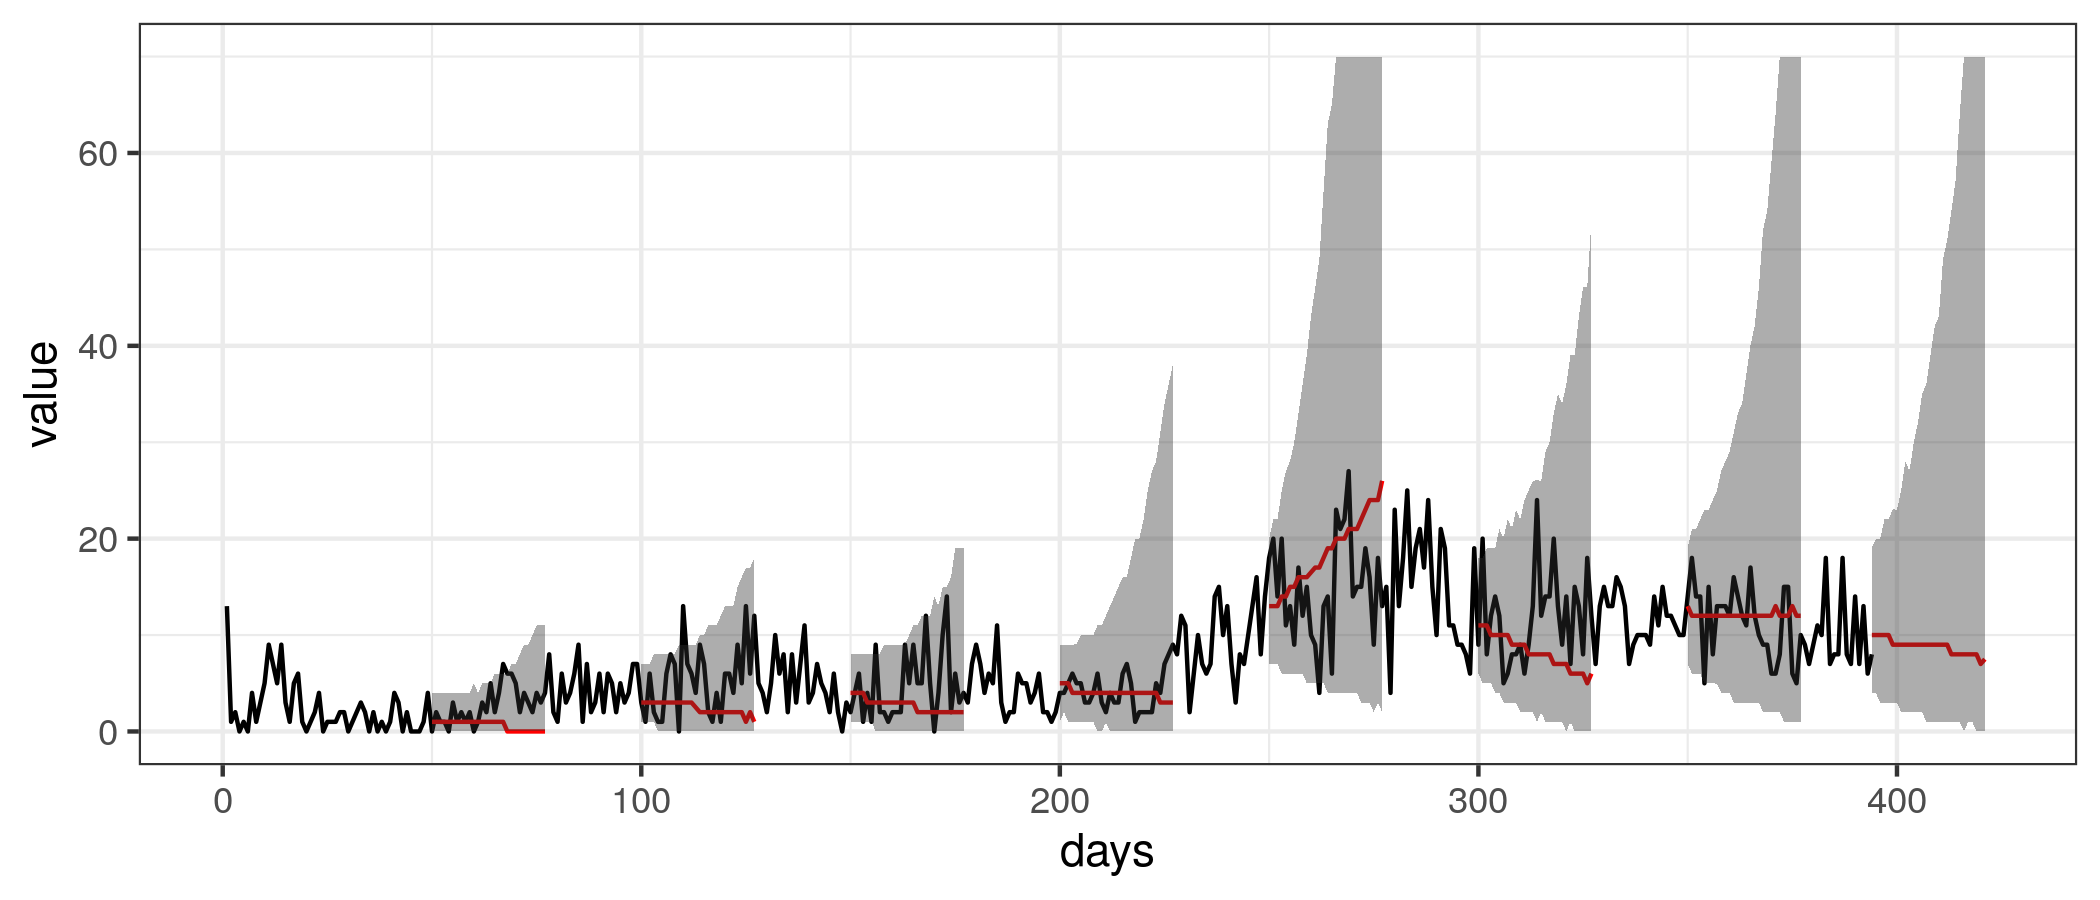
\includegraphics[width=0.9\linewidth, height=7cm]{../output/national_predictions.png}  
  \caption{Forecasted and predicted incidence for the semi-local Poisson model}
  \label{fig:sub-first}
\end{subfigure}

\begin{subfigure}{\textwidth}
  \centering
  % include second image
  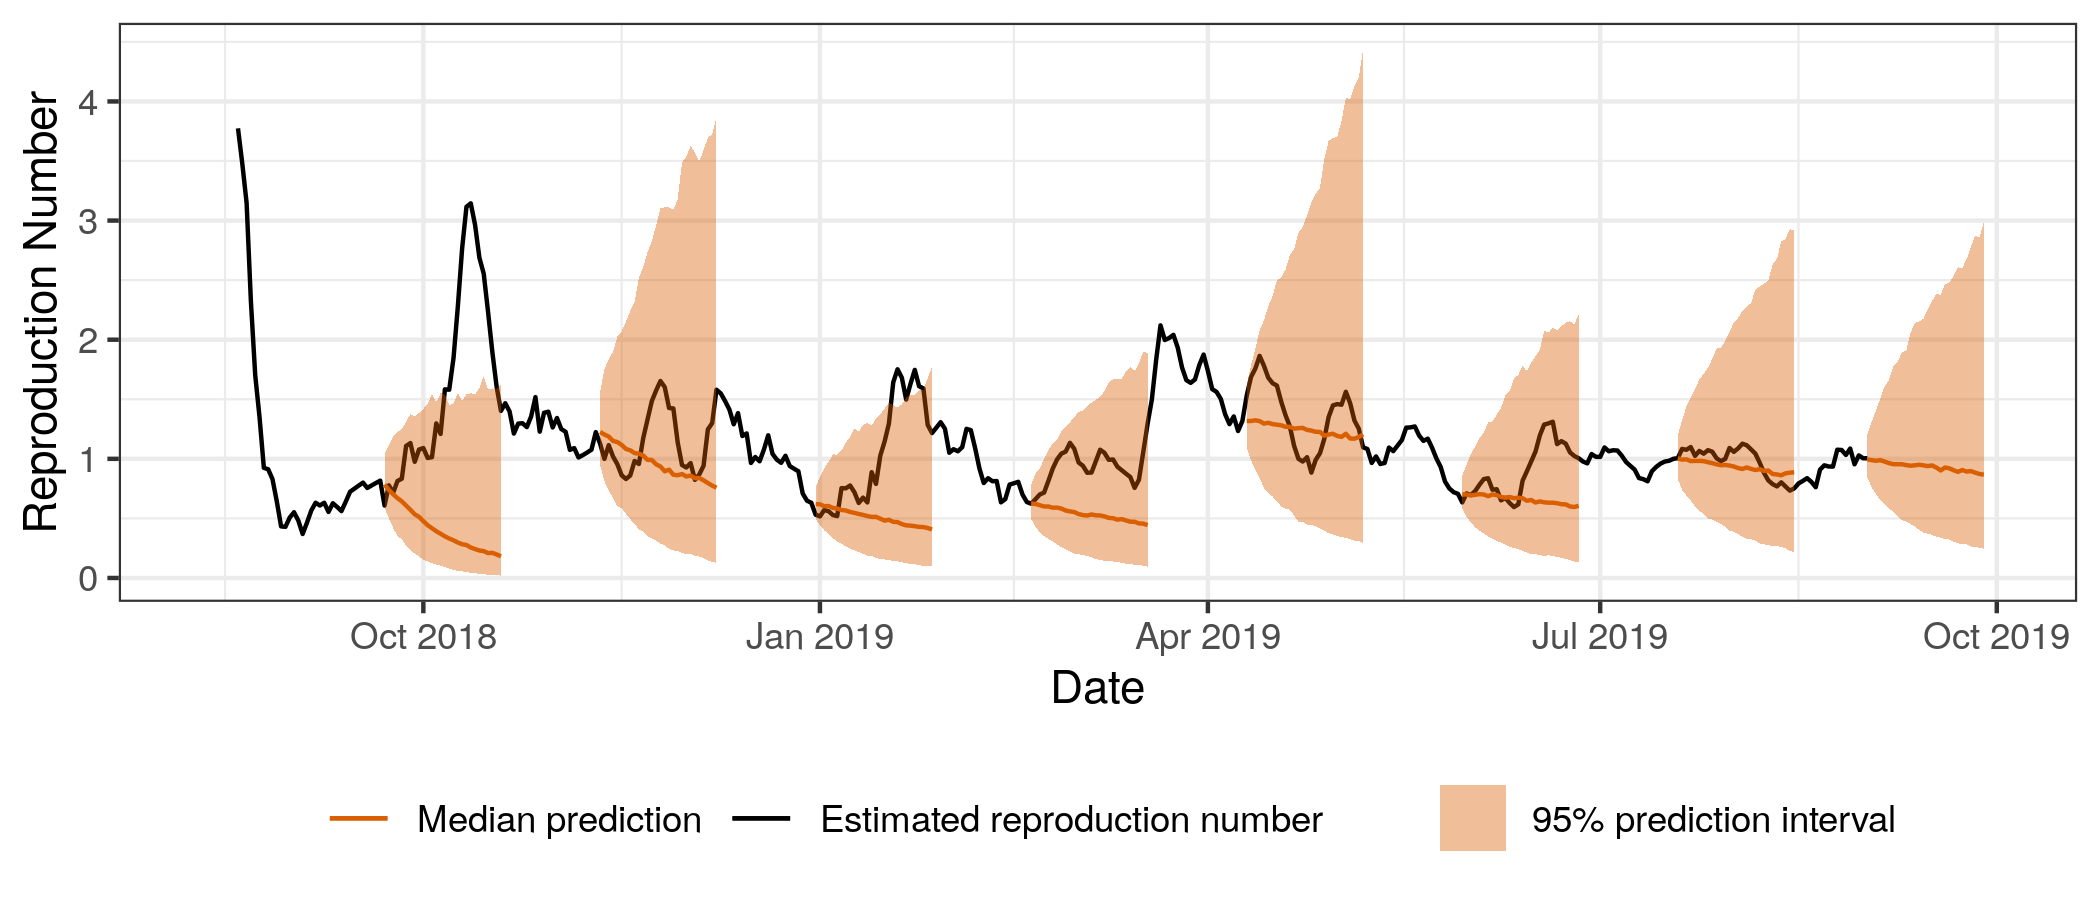
\includegraphics[width=0.9\linewidth, height=7cm]{../output/national_Rs.png}  
  \caption{Forecasted and predicted reproduction numbers for the semi-local Poisson model}
  \label{fig:sub-second}
\end{subfigure}
  \caption{Median forecast with 95\% prediction intervals and observed values for incidence and reproduction number for the semi-local Poisson model}.

  \label{fig:nat_pred}
\end{figure}

\subsection{Health Zones}

We fitted all four models separately for each health zone with more than one case of Ebola. The performance of the models varied significantly from health-zone to health-zone. Table \ref{tab:best_model} shows the best model(s) for each health zone, how large a forecasting horizon we can have without ruling out calibration and the total number of confirmed cases in the health-zone. There is a large difference from health-zones where the forecasts are calibrated for 28 days, to health-zones where not even the one day ahead predictions are calibrated.

% latex table generated in R 3.6.1 by xtable 1.8-4 package
% Tue Sep 24 17:36:32 2019
\begin{table}[h!]
\centering
\begin{tabular}{|l|l|l|l|}
  \hline
Location & Largest Horizon & Best model & Cases \\ 
  \hline
Kayna & 28 & NegBin Semilocal & 22 \\ 
  Nyiragongo & 28 & NegBin Semilocal & 3 \\ 
  Tchomia & 28 & NegBin Semilocal & 2 \\ 
  Lolwa & 26 & All models & 3 \\ 
  Mwenga & 18 & All models & 6 \\ 
  Bunia & 17 & NegBin Semilocal & 4 \\ 
  Alimbongo & 12 & NegBin Semilocal & 5 \\ 
  national & 9 & Poisson Semilocal & 2942 \\ 
  Kayina & 7 & Poisson Semilocal & 10 \\ 
  Rwampara & 6 & NegBin Latest & 8 \\ 
  Lubero & 4 & NegBin Semilocal & 31 \\ 
  Musienene & 4 & Poisson Semilocal & 84 \\ 
  Kyondo & 3 & Poisson Semilocal & 22 \\ 
  Vuhovi & 3 & Poisson Semilocal & 103 \\ 
  Beni & 2 & Poisson Semilocal & 661 \\ 
  Biena & 2 & Poisson Latest & 16 \\ 
  Butembo & 2 & NegBin Semilocal & 279 \\ 
  Mabalako & 2 & NegBin Semilocal & 371 \\ 
  Kalunguta & NA & No calibrated model & 164 \\ 
  Katwa & NA & No calibrated model & 647 \\ 
  Mangurujipa & NA & No calibrated model & 20 \\ 
  Masereka & NA & No calibrated model & 50 \\ 
  Mutwanga & NA & No calibrated model & 31 \\ 
  Oicha & NA & No calibrated model & 55 \\ 
  Komanda & NA & No calibrated model & 43 \\ 
  Mambasa & NA & No calibrated model & 32 \\ 
  Mandima & NA & No calibrated model & 264 \\ 
   \hline
\end{tabular}
\caption{For each health zone we show the maximal forecasting horizon where we can not exclude calibration at the p=0.1 level. If multiple models are equally calibrated we chosse the one with smallest RPS. For some health zones there were no calibrated forecasts} 
\label{tab:best_model}
\end{table}


For all health zones apart from one, we find that the best model is a model with a semi-local trend in the reproduction number. Sometimes the Poisson models are better and sometimes the negative binomial models are better.

The health zones were we get very well calibrated models are health zones with small bursts of Ebola activity followed by long periods of no cases. Once our model has seen no new infections in a few weeks they will predict almost 0 new cases irrespective of the current reproduction number. This behaviour works well when there are no new imported cases as we can see in some of the health zones. For the larger health zones where there is more sustained transmission the models works for some health zones, but not as well on the national level. There are also some health zones with many cases where the models do not work well. We show the predictions and the centrality measures for the Beni and Katwa health zones in Figure \ref{fig:beni_katwa}. The models and evaluations for all the other health zones can bee seen in the Appendix. For both Beni and Katwa the main reason the models are not well calibrated is that they overestimated their own uncertainty. This is especially the case in Katwa and explains why even the one-day ahead prediction is not well calibrated. 

\begin{figure}[h!]
\begin{subfigure}{0.5\textwidth}
  \centering
  % include first image
  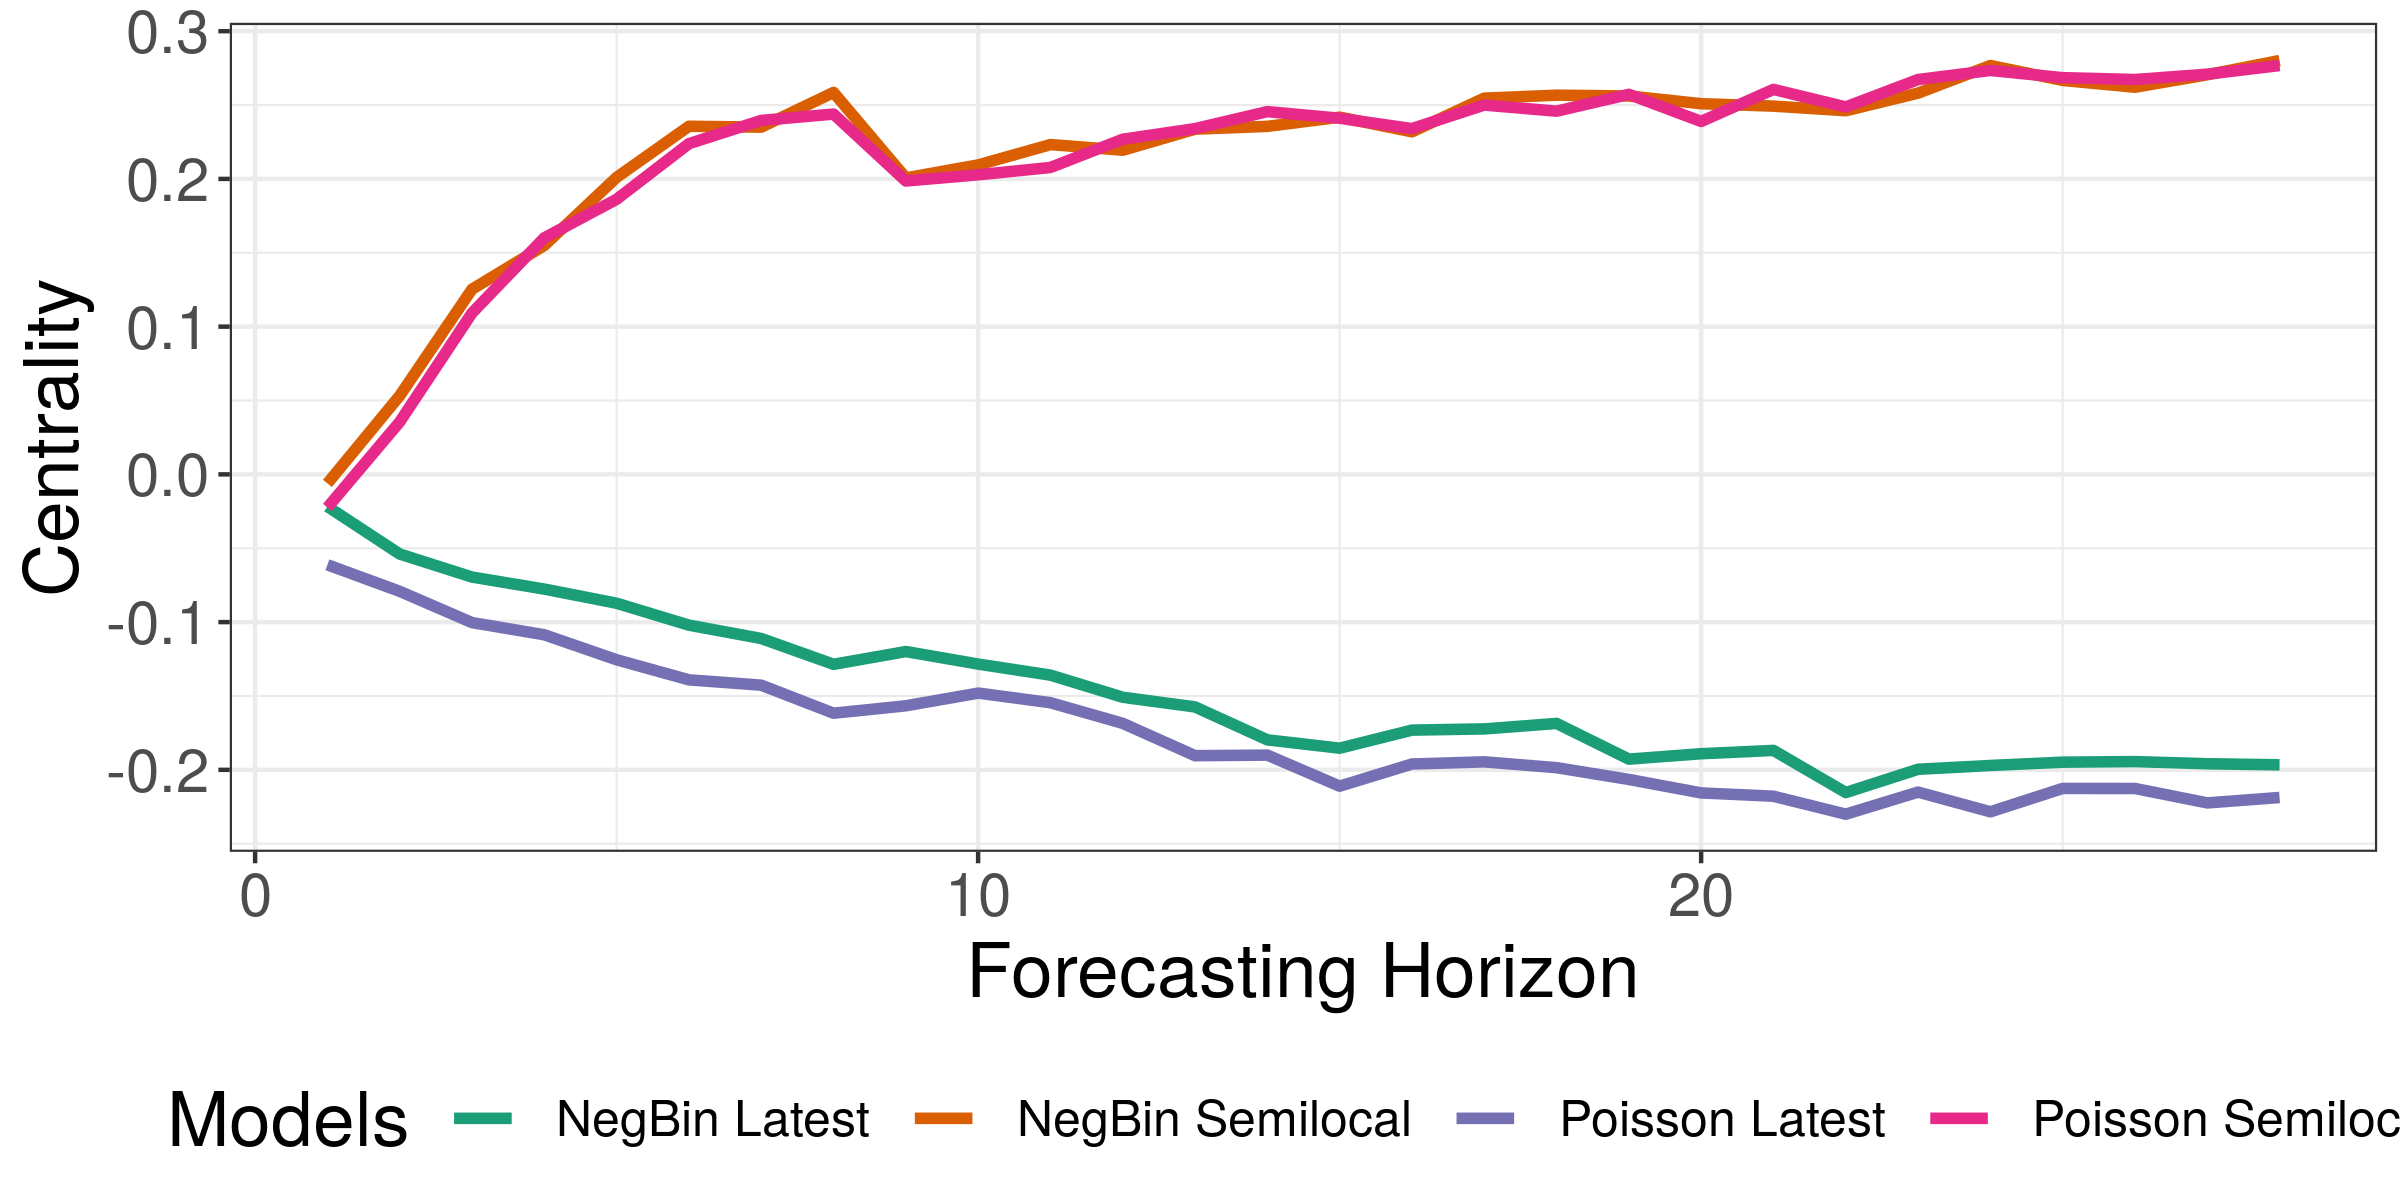
\includegraphics[width=\linewidth, ]{../output/Katwa_centrality.png}  
  \caption{Centrality of PIT values for the Katwa model}
  \label{fig:beni_katwa_1}
\end{subfigure}
\begin{subfigure}{0.5\textwidth}
  \centering
  % include second image
  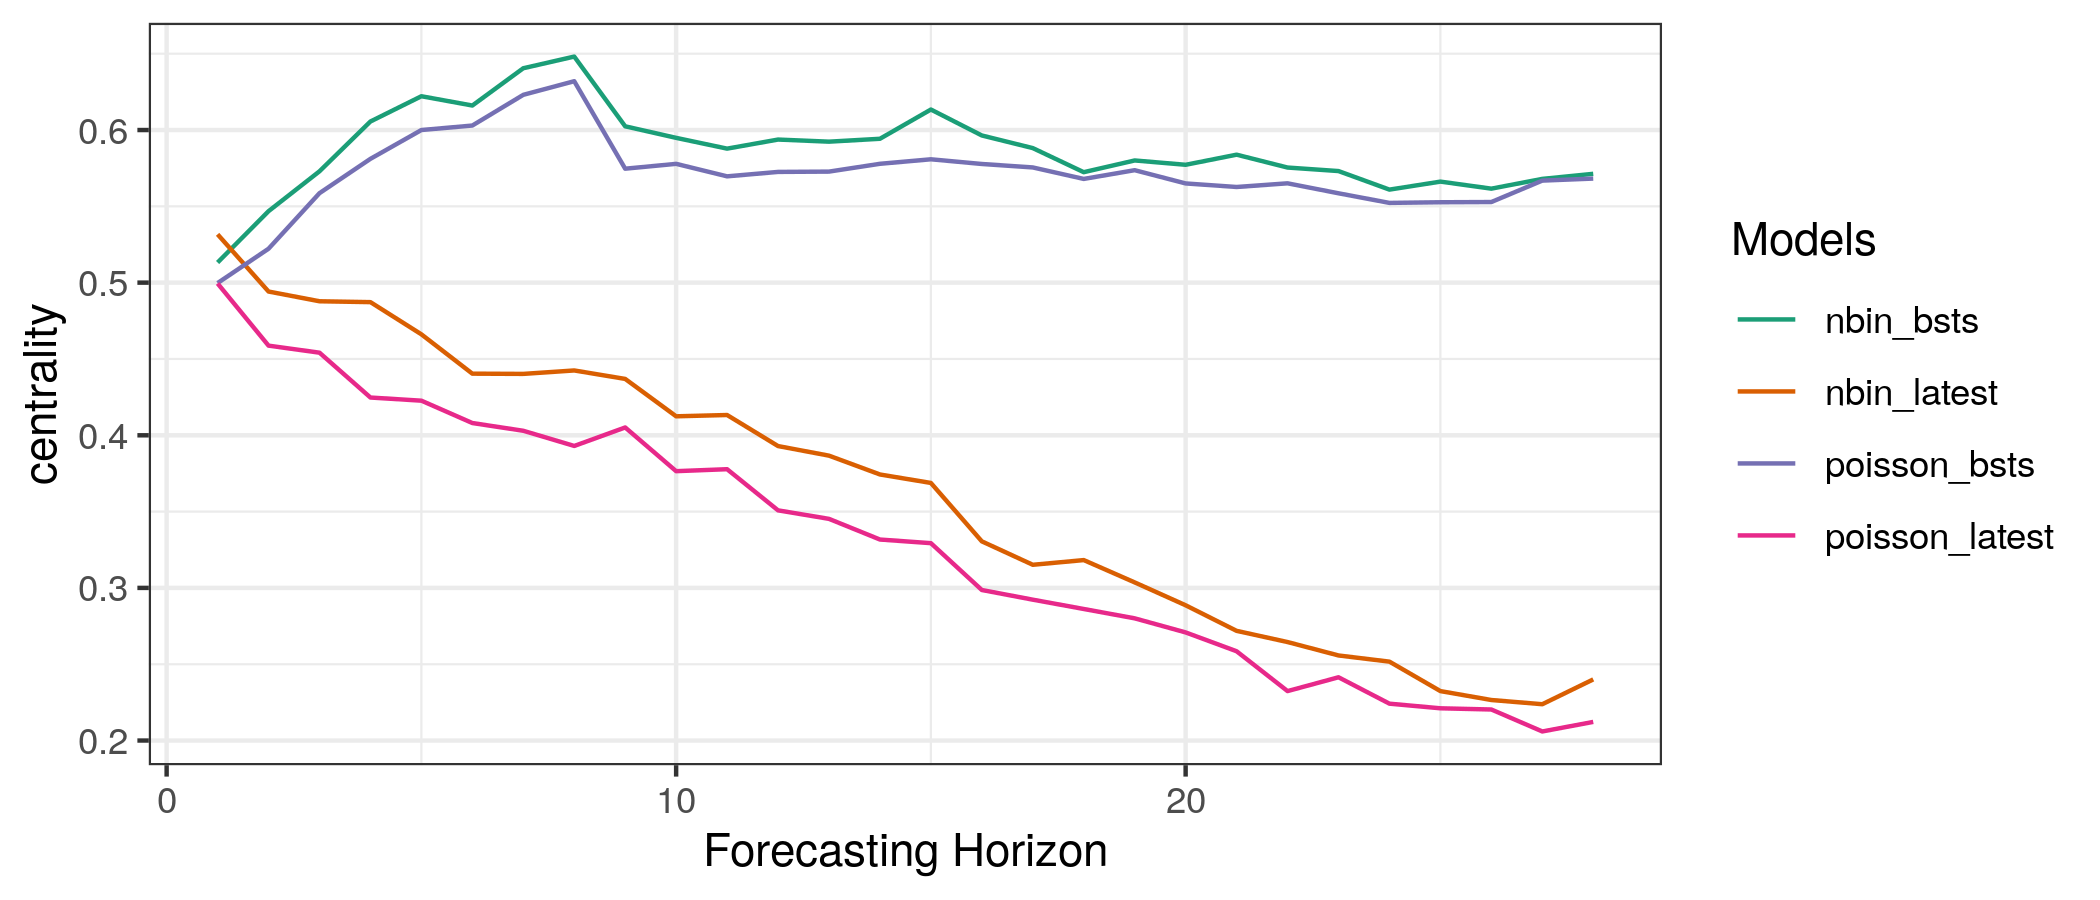
\includegraphics[width=\linewidth]{../output/Beni_centrality.png}  
  \caption{Centrality of PIT values for the Beni model}
  \label{fig:beni_katwa_2}
\end{subfigure}

\begin{subfigure}{\textwidth}
  \centering
  % include first image
  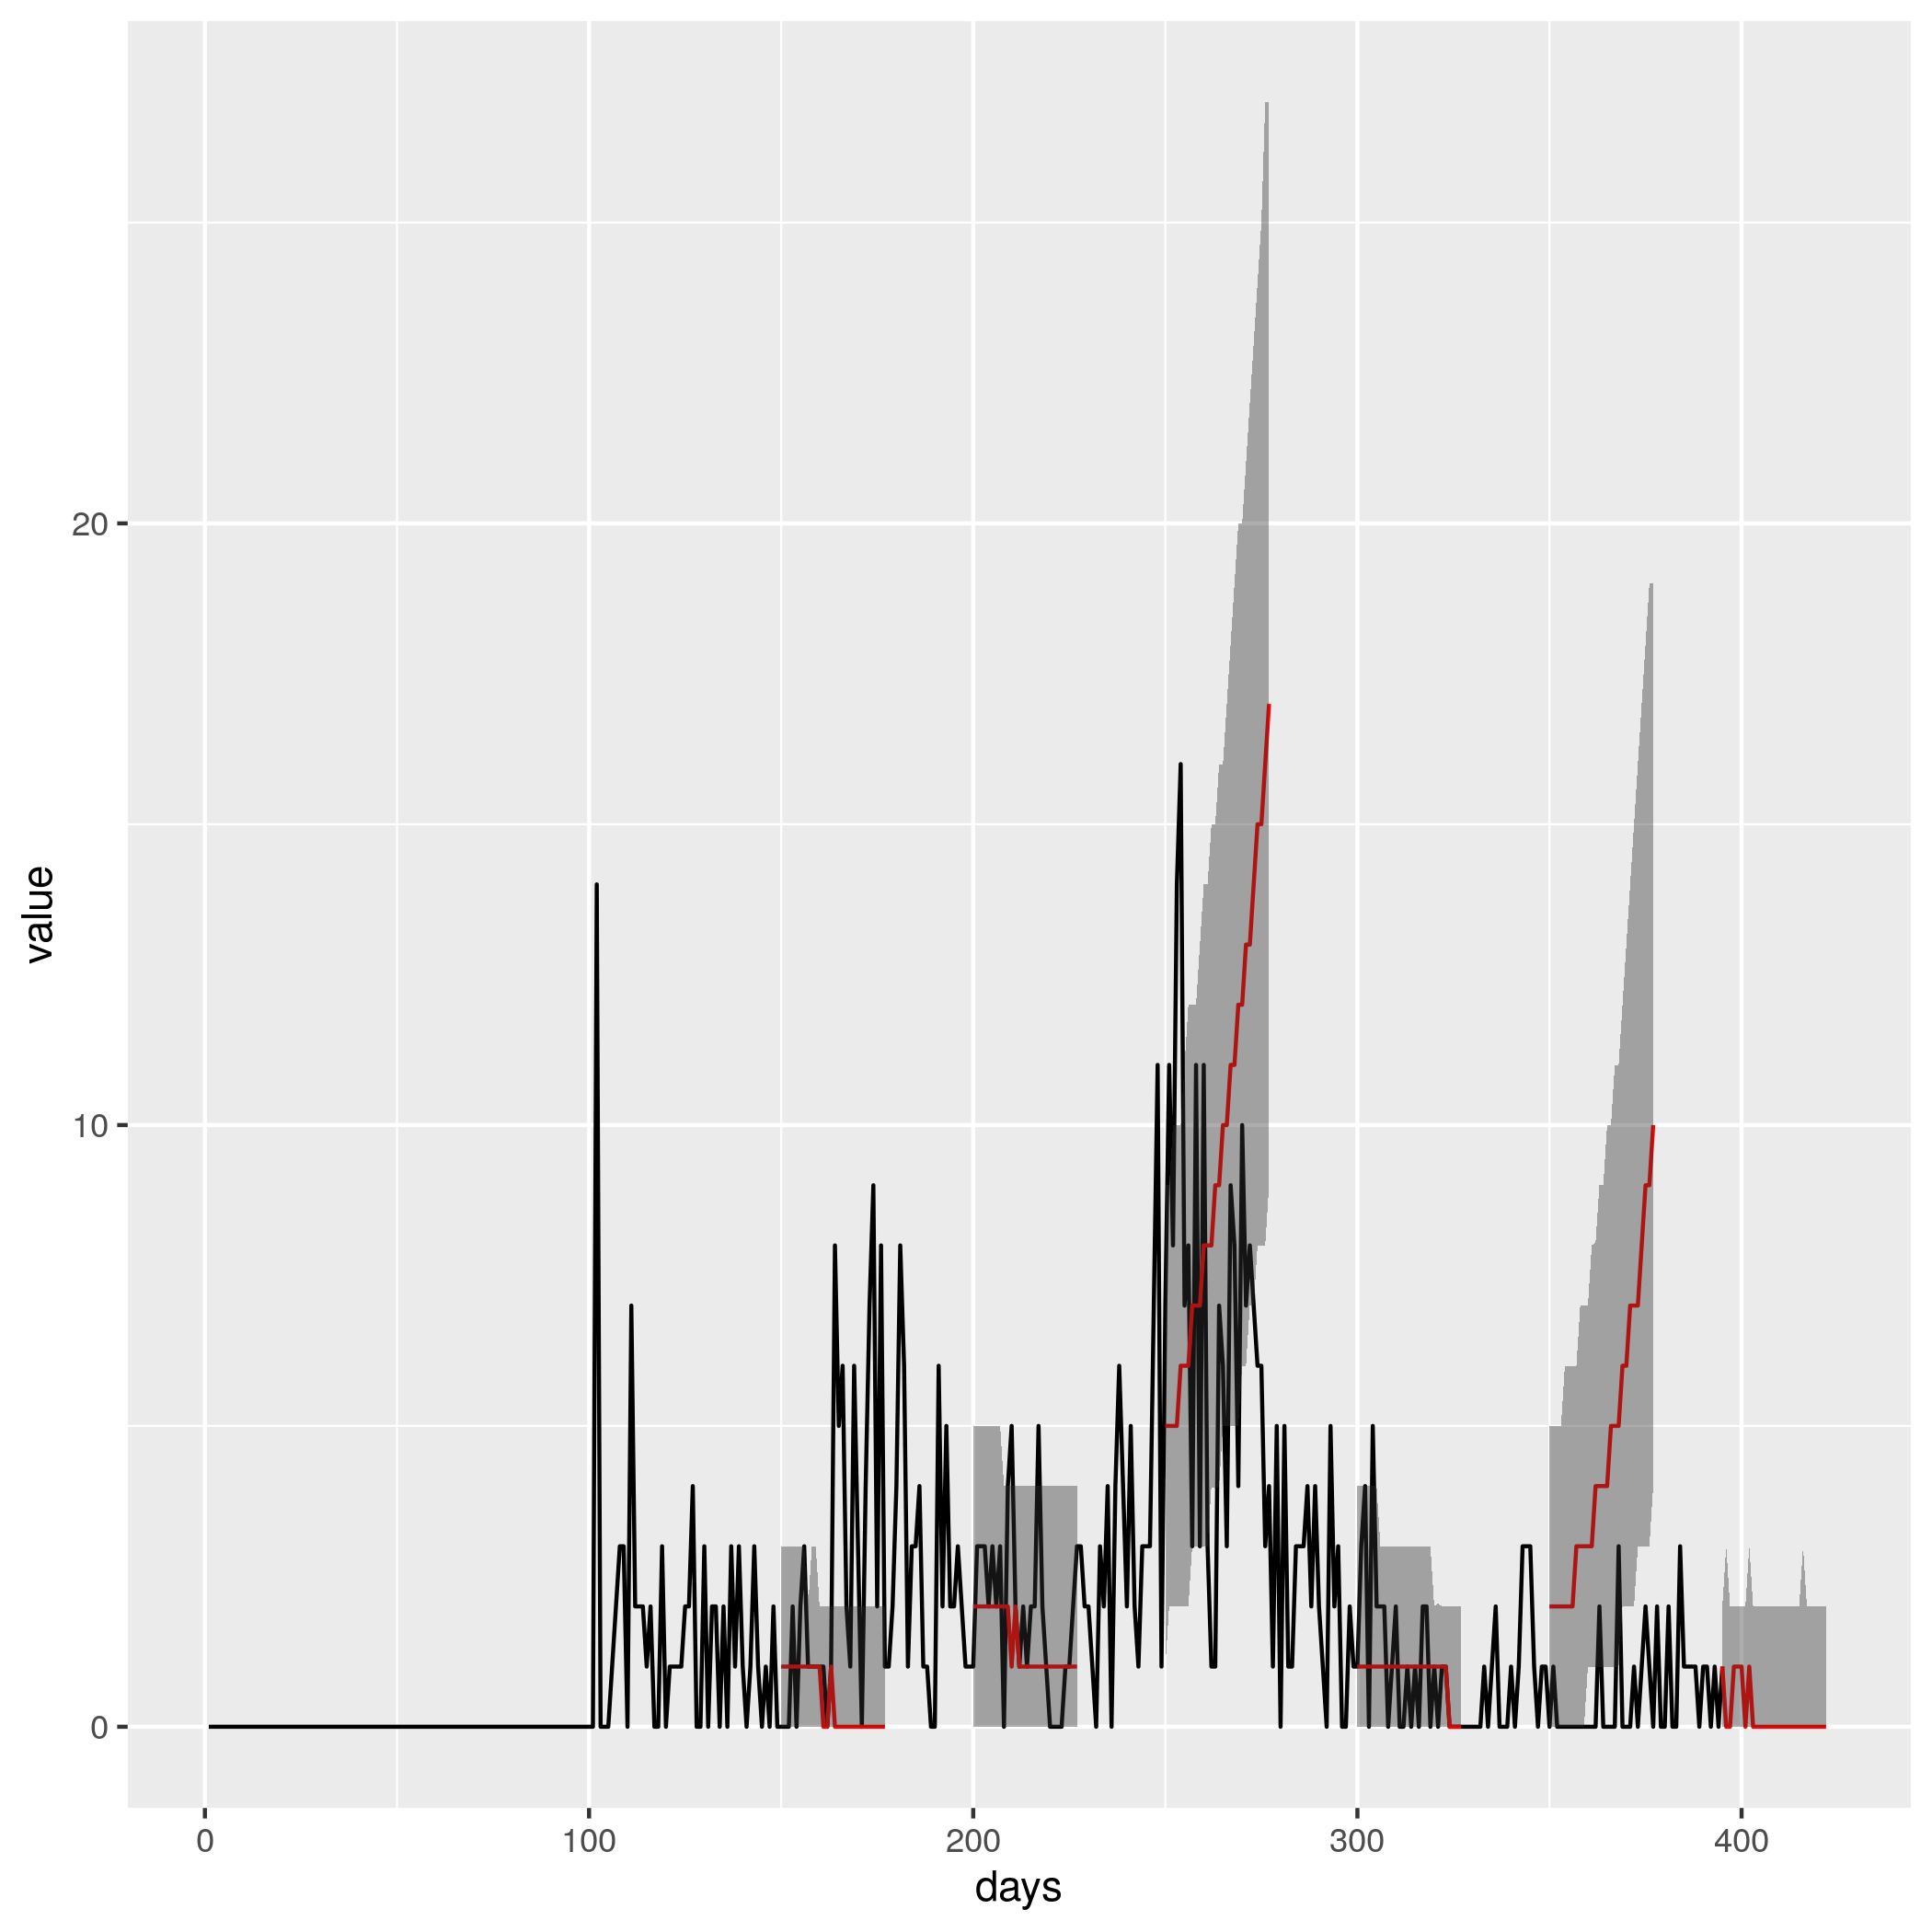
\includegraphics[width=0.9\linewidth, height=7cm]{../output/Katwa_predictions.png}  
  \caption{Predictions Katwa model}
  \label{fig:beni_katwa_3}
\end{subfigure}

\begin{subfigure}{\textwidth} 
  \centering
  % include second image
  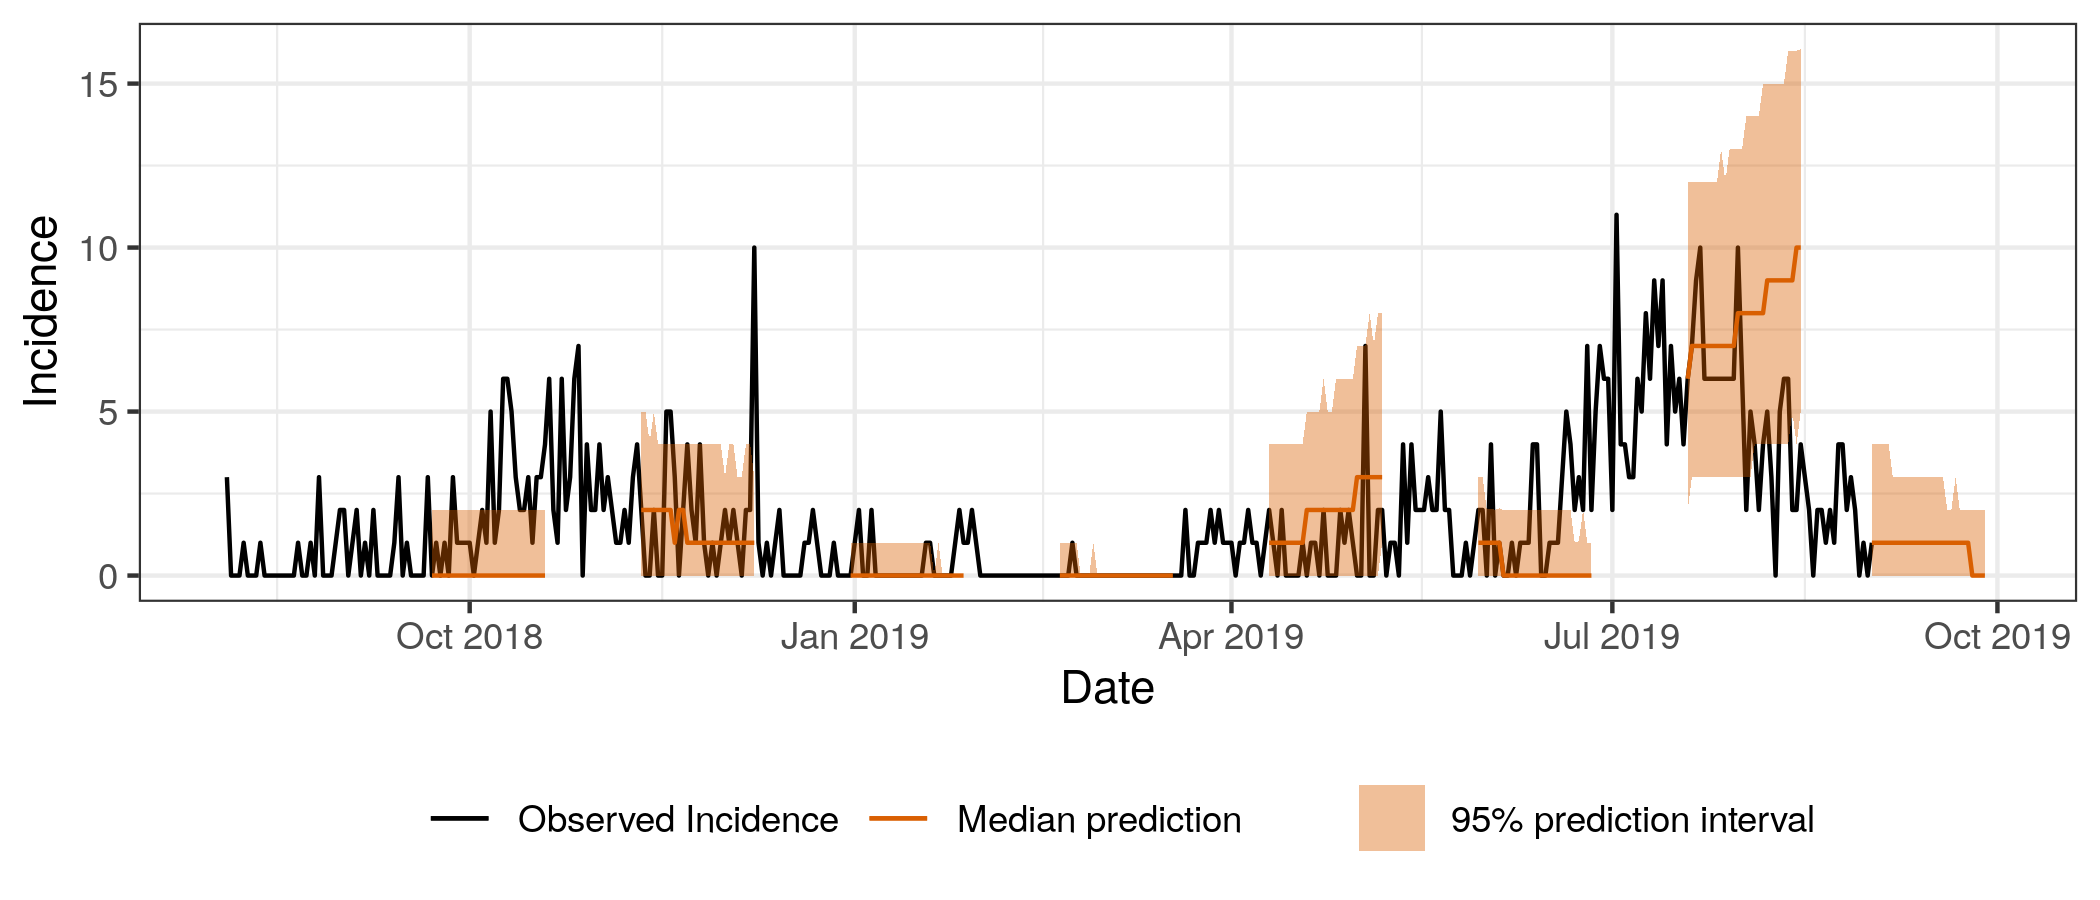
\includegraphics[width=0.9\linewidth, height=7cm]{../output/Beni_predictions.png}  
  \caption{Predictions in Beni}
  \label{fig:beni_katwa_4}
\end{subfigure}

\caption{Centrality for Katwa and Beni}

\label{fig:beni_katwa}
\end{figure}
As a final check of the health zones predictions we compared the the one-day ahead predictions of the national level model with the one-day ahead predictions of a sum of the semi-local Poisson model for all the health zones in Figure \ref{fig:nat_nat_comb}. We see that model based on summing up all the health zones predict consistently too large incidence and would not work well for forecasting the outbreak. The combined model also does not have any forecasting horizons with calibrated forecasts and have significantly higher CRPS and DSS score compared to the model fit to national data

\begin{figure}[h!]
  \centering
  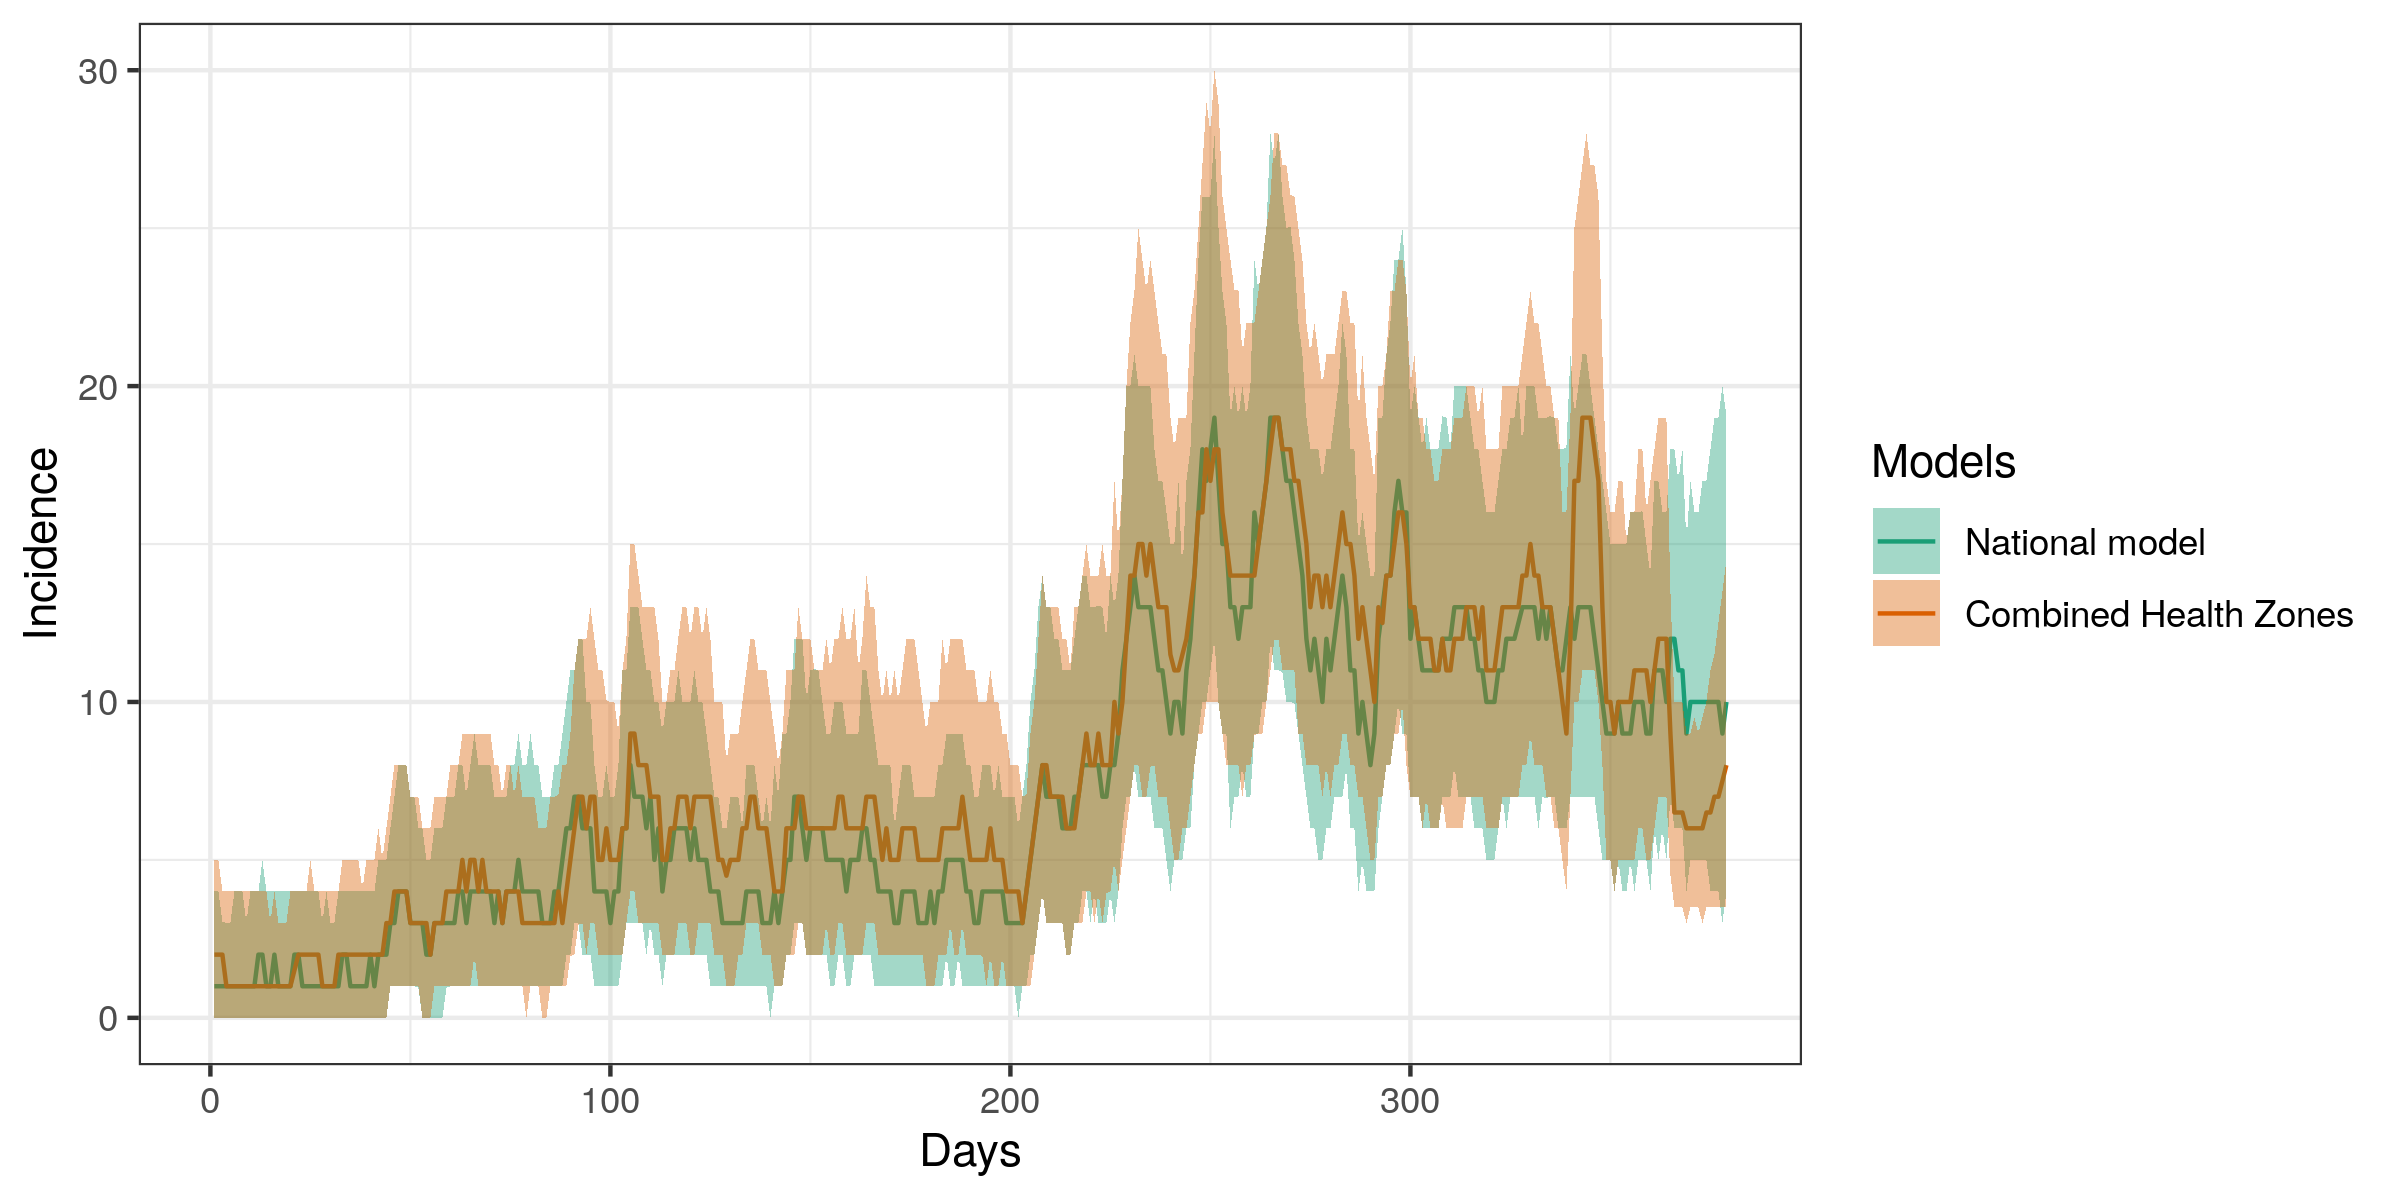
\includegraphics[width=0.9\linewidth]{../output/nat_combined.png}
  \caption{Median and 95\% prediction intervals for the national model and for a model calculated by summing up models for all the health zones}
  \label{fig:nat_nat_comb}
  
\end{figure}

\section{Discussion}


The ongoing Ebola outbreak in northern DRC is the second largst Ebola outbreak and is of significant regional and international concern. As of the 1st of September 2019, it is not under control as we can see both from the fact the reproduction number is not below one and that there are still plenty of new cases and deaths not on contact lists. In addition to a large number of confirmed Ebola cases, this outbreak has seen a high CFR of 66\% compared to 51\% in the west African outbreak\cite{rojekSystematicReviewMetaanalysis2019}. Both the long duration, difficulty of control and high CFR are likely due to the difficult context for the outbreak response. This part of DRC has a history of violence and mistrust of the central government and international organisations. This makes all parts of the response from finding cases, tracking contacts, ensuring early treatment and safe burials much more difficult. Based on the models investigated in this paper it seem like the large increase of cases seen from March - June 2019 is over and that there is hope that the outbreak can be controlled, but the large uncertainty of the situation which is reflected in the large uncertainty in the models make long term predictions very difficult if not impossible.

Compared to estimates of the reproduction number in the West-African Ebola outbreak\cite{WestAfricanEbola2015} the reproduction number in the DRC outbreak has seen larger variations on short time-scales and less longer patterns. In the previous outbreak we saw in both Guinea and Liberia that the reproduction number peaked around 2 after a few months followed by a long slow decline. This outbreak has been more characterised in multiple short term peaks or waves of higher reproduction number with the peaks reaching over 3 at some points. It is possible that the different patterns from the different outbreaks can tell us about the response. The West-African repsone was maybe slower to get properly started, but once it did the response started working and was fairly uninterupted. In the current outbreak the response was faster, but potentially due to the security situation the response has been interrupted and this could be why we see the short term peaks. The range of reproductive values seen is also similar to other previous Ebola outbreaks \cite{legrandUnderstandingDynamicsEbola2007}.

We find that on the national level the models with a semi-local trend for the reproduction number were calibrated out to about a forecasting horizon of 9 days and significantly outperformed the simpler models based on a non-changing reproduction number. The length of the forecasting horizon is similar, but a bit shorter than the 2 weeks found in \cite{funkAssessingPerformanceRealtime2019} where a semi-mechanistic model based on a SEIR that included reporting delays. That model was semi-mechanistic as the transmission rate was allowed to vary as a random walk. While direct comparisons are not possible due to the different outbreaks it is of interest if our model with much less deterministic structure can give fairly similar calibrated forecasting horizons. Other models have been used to forecast the current Ebola outbreak, e.g \cite{kellyRealtimePredictions201820192019, akhmetzhanovAnalyzingForecastingEbola2019}. They use very different modelling techniques and a proper comparison between the models would require comparing proper scoring rules score using the same data, but in \cite{akhmetzhanovAnalyzingForecastingEbola2019} they use similar forecasting horizons of around two weeks.

The best model for the national outbreak is uncalibrated when forecasting more than 9 days forward due to overestimating the amount of uncertainty in the incidence. Depending on how the forecasts are used, it is possible that uncalibrated but over-dispersed forecasts can still be useful for planning purposes since they are conservative. An upper limit for an over-dispersed forecasts will give a conservative upper limit for future incidence. Forecasts based on under-dispersed models, require a lot more care and should be treated with caution. Models that only provide point-predictions or do not actively try to quantify the uncertainty are by definition under-dispersed. The main reason for the over-dispersion in the semi-local models is likely due to the forecasting of the reproduction number. This model allows large variation in the reproduction number over fairly short time, but does not have any information about what range of reproduction numbers are actually feasible. In this outbreak we see fairly fast changes of the reproduction number, but the reproduction number almost never is larger than 3. A model for reproduction number than allows the fast variation and short peaks, but that keeps the reproduction number within a more narrow band, might give a better model.

A probabilistic modelling approach with tests for calibration and using proper scoring rules to see which forecast is better is a crucial step to compare forecasts and to evaluate their validity. The proper scoring rules are mainly useful when comparing models, while the calibration gives an absolute measure for how well the forecast captures the uncertainty seen in the process. In this study we found these tools crucial both for model selection and for the final interpretation of our model. Once the forecasting horizon is longer than 9 days we can not really trust that the model adequately predicts the uncertainty in the process. Even a well calibrated model can make large forecasting mistakes if the underlying process changes in a way not seen before during the time period used to test the model. Therefore it is always crucial to critically evaluate models and the metrics used to evaluate the models. We find that both the CRPS and DSS scores give similar performance, but that calibration using the PIT values was especially valuable. The introduction of the centrality measure of the PIT histograms give additional valuable information and allows us to understand better how our models are failing if they are not well calibrated. The centrality is a fairly crude measure of this and a measure that also includes other departures from normality of the PIT values could give additional information. 

We find that for one-day ahead forecasts the negative binomial distribution is needed for a calibrated forecast. This indicates that a Poisson offspring distribution where everyone is always equally likely to transmit the disease in every small time frame does not adequately describe the transmission process. We found a relatively large value for the $k$ parameter which gives a fairly modest increase in variance. Much smaller than found when investigating transmission chains in the west Africa ebola outbreak \cite{internationalebolaresponseteamExposurePatternsDriving2016}. It is possible that variance is smaller in this outbreak, but this should be taken as fairly weak evidence of that and a proper investigation of transmission chains would be needed. 

We successfully could provide forecasts for all health-zones with more than one cases, but the quality was very varying. For some health zones where there were very few cases and then longer period with no transmission, the model managed fairly well, but for most health zones with a large number of cases the models where again too over-dispersed to provide calibrated predictions. For almost all health zones the models with semi-local trend were better than the models with constant reproduction number. 


The models investigated in this paper are all lightweight enough to easily run on a normal laptop in at timescale of minutes to allow real-time forecasts during an outbreak. 

%% Model assesment


The models and forecasts in this report have multiple limitations. Firstly, the data source for the model is the cumulative number of cases by reporting day which we use to calculate the incidence. This data source has many disadvantages to for example having a line list of all cases. A line list would give a much better idea of the data of onset of disease, it would remove the problem with negative incidence rates after corrections and any problems with having to interpolate incidence rates.

It is a strength of the modelling approach that it can be used on less than ideal data to still give reasonable short-term forecasts. The stringent tests of calibration can give us confidence in the forecasts even without perfect data. This is of key importance in outbreak situations where having up-to-date line lists of cases can be difficult or impossible. The approaches in this report could still give reasonable forecasts. 

The model in it's current form has several limitations. As previously discussed it seems to predict to much variance in the reproduction number which leads to over-dispersed predictions. There are also clear limitations on the health-zone level and that is that spread between health zones is not modelled. We only model the spread of the disease after it has been introduced to a health zone. For the national level we do not have this limitation, but it makes it very difficult to use the current model to study the spatial spread of the disease. 

Due to the flexibility of the he model structure it would be fairly straight-forward to incorporated an additional force of infection term that gives the force of infection from outside the health zone. There are multiple options for how to model the geographic dependence that would all easily fit into our model structure, this includes spread from adjacent health zones, using a gravity model where the amount of spread between health zones is based on the populations or if available data on inter health-zone travel could be used. Without this spread term the model can not be used to forecast probabilities for the spread of Ebola to new health zones. In addition the current way of estimating the time-varying reproduction number requires at least 17 days of data, so we need at least 17 days of data in a health zone to be able to forecast.

In addition to the spatial spread, it would be beneficial to combine the separate parts of the model together into one generative model. This means including the estimation of the reproduction number into the main model. One promising way of doing this is a full Bayesian generative model. One of the main benefits of a generative model is that it models the whole data generation process and would allow us to simulate whole outbreaks. For future work it would also be very interesting to investigate different models for the time evolution of the reproduction number. A full Bayesian treatment would also allow us to model uncertainty in the parameters of the offspring distribution, uncertainty about serial interval and could even include imputation for missing data. 

In this report we used a semi-mechanistic model with fairly few assumptions about the disease transmission. The flexibility of the reproduction number in this model allows us to fit complicated incidence histories that could not have been easily fit by traditional compartmental models. The benefit of the structure we do have in the model is that certain basic facts about how disease spread that are likely to be fairly correct for most diseases. The model used in this report could easily be adopted to other diseases and other contexts without any real changes in the model structure. We would need a different serial interval, but the rest of the model could stay the same. The benefit of adding more structure to a model, for example an SEIR structure is that it is easier to model the results of interventions like vaccination \footnote{Using the fact that $R_t=R_o*s(t)$ in a compartmental model of the SEIR type, it would likely be possible to model some simple interventions in the models in these papers too}. One key aspect to consider when choosing models for an outbreak situation is that maybe more than one model should be used during the outbreak. At the start of the outbreak when the important mechanisms are less well know, maybe a model with less mechanistic structure is the most useful and then once we learn more about the outbreak we can add more structure to the model. In many forecasting challenges it has been shown that an ensemble of models perform better than individual models \cite{dietterichEnsembleMethodsMachine2000}, this was also found in the RAPPID modelling competition for Ebola \cite{viboudRAPIDDEbolaForecasting2018}. 

Theoretically it should be possible to forecast infectious disease outbreaks on the timescale of individual outbreaks \cite{scarpinoPredictabilityInfectiousDisease2019}. The models in this report and other disease forecasting models still have a long way to go to acheive this goal. For the current Ebola outbreak many additional sources of data exists that are not used in models, this includes deaths vs cases, community deaths vs deaths in treatment centres, contacts followed-up, vaccinations, data on response activities etc. It is possible that combining these additional data sources together with improved modelling techniques we could significantly increase forecasting horizon where we got provide calibrated predictions. 

%% Concluding remarks



%% What does it all mean?
%%  -- Interpret repproduction number
%%  -- Reiterate why we do it:
%%  -- Likely path of the epidemic - incude why uncertainty is important
%%  -- need dimensions of control effort - is the control working?
%%  -- subnational prioritisation of control efforts 

%% Model selection. Pheno vs compartmental
%% What epidemiological question are we answering?
%% flexible model part can do well


%% Improvments: Full baysian model, hierracical model that includes spread from HZ to HZ, now only including internal spread.
%% Why a generative model is good?



\section{Conclusions}
We found that a probabilistic forecasting model based on a branching process with a Poisson offspring distribution with a time-varying reproduction number forecasted with a semi-local trend gave well calibrated forecasts for the 2018--2019 Ebola outbreak in DRC for forecasting horizons up to 9 days. This model together with a similar model but with a negative binomial offspring distribution could also give calibrated forecasts for some of the individual health zones, but for many health zones the models had too much uncertainty. 


\newpage

\bibliography{bibliography} 
\bibliographystyle{ieeetr}

\clearpage
\newpage

\appendix
\appendixpage
\addappheadtotoc
\addtocontents{toc}{\protect\setcounter{tocdepth}{0}}
This appendix shows the best fitting model and evaluation score for each health zone.

 \section{ Butembo }\begin{figure}[H]\begin{subfigure}{\textwidth}  \centering  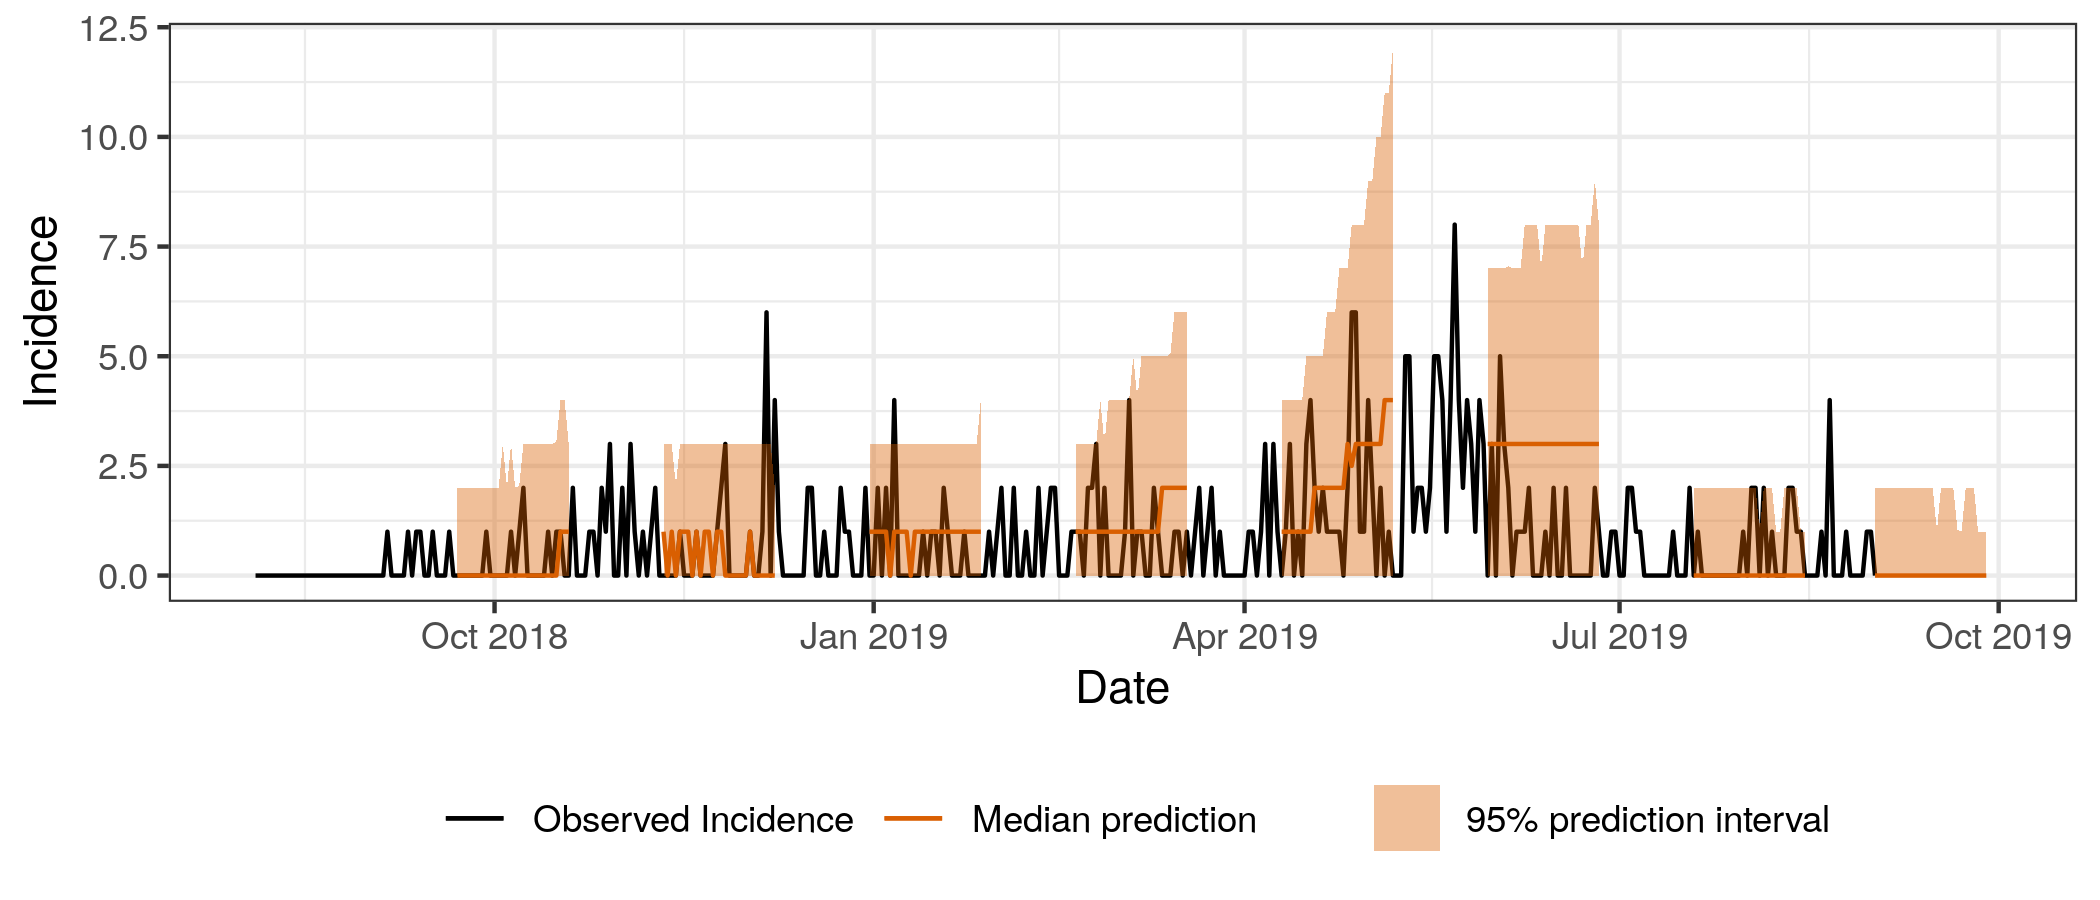
\includegraphics[width=0.9\linewidth, height=7cm]{../output/Butembo_predictions.png}  \caption{Forecasted and predicted incidence for the best fitting model}\end{subfigure}

\begin{subfigure}{\textwidth}  \centering  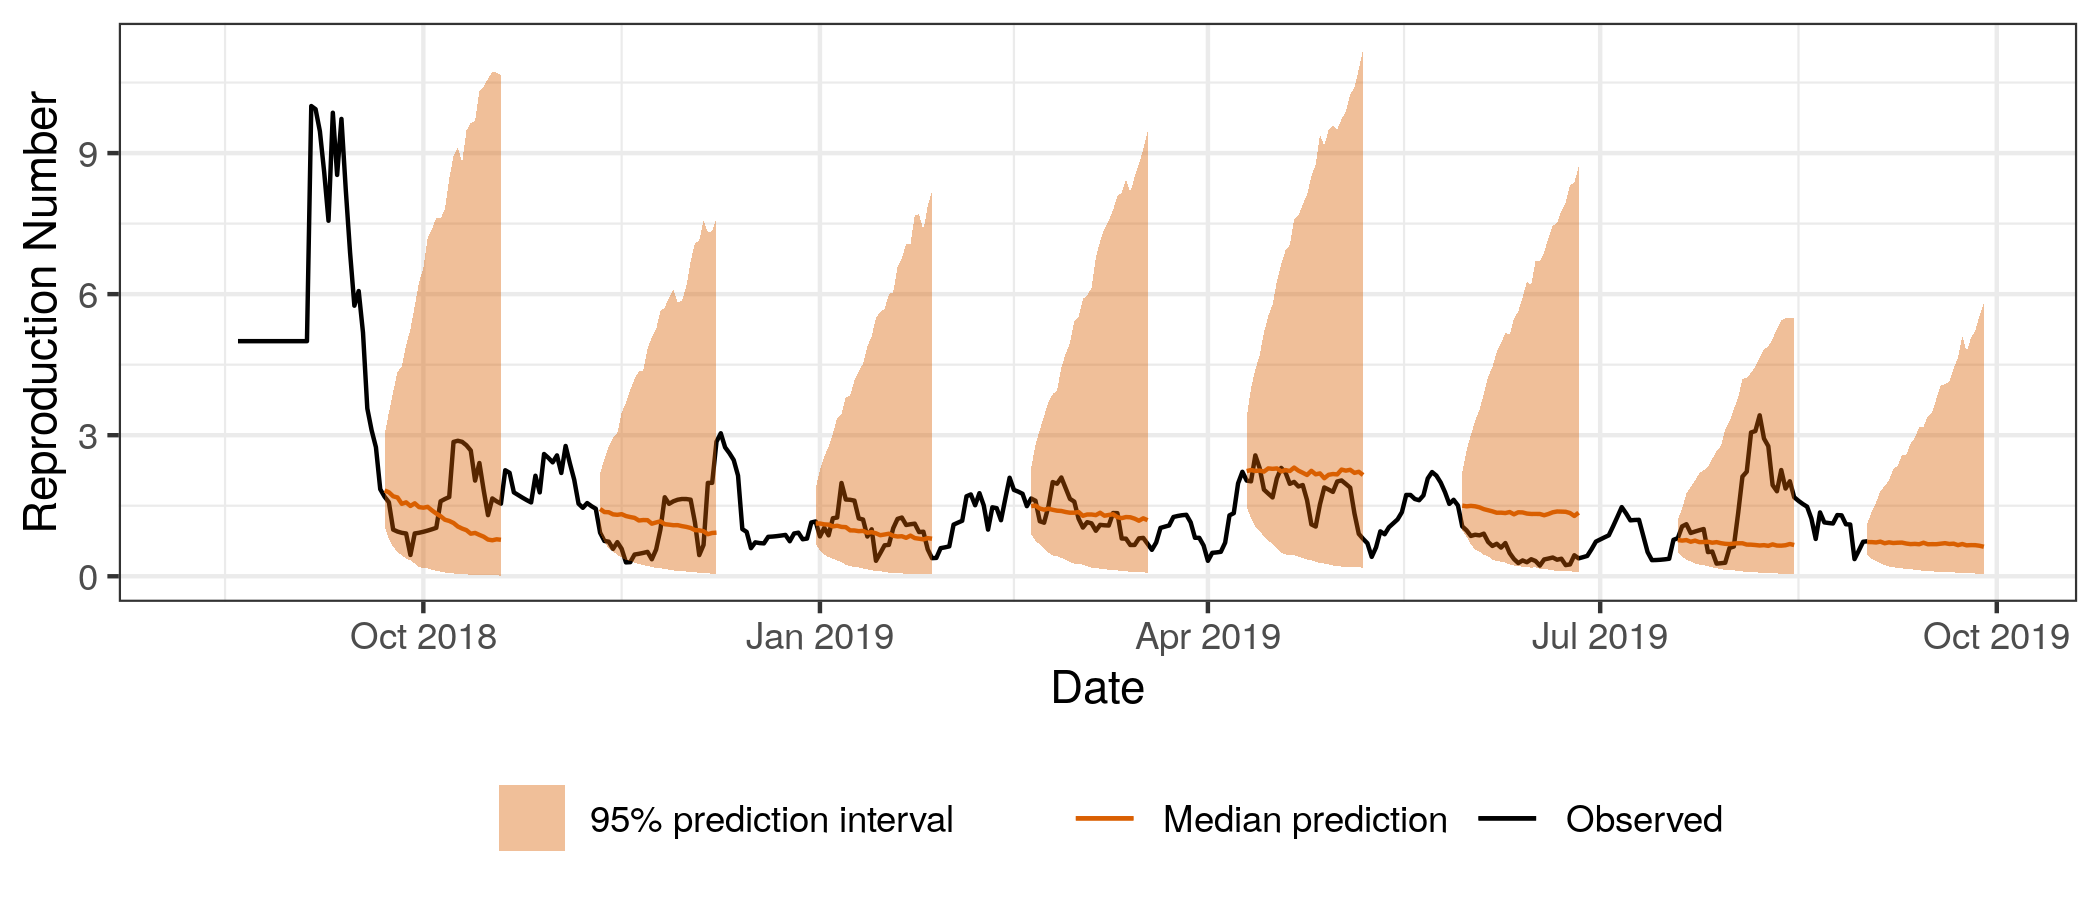
\includegraphics[width=0.9\linewidth, height=7cm]{../output/Butembo_Rs.png}  \caption{Forecasted and predicted repreoduction numbers for the best fitting model}\end{subfigure}  \caption{Median forecast with 95 \% prediction intervals and observed values for incidence and reproduction number for the best fitting model for Butembo.}\end{figure}

\begin{figure}[H]
\begin{subfigure}{0.5\textwidth}
  \centering
  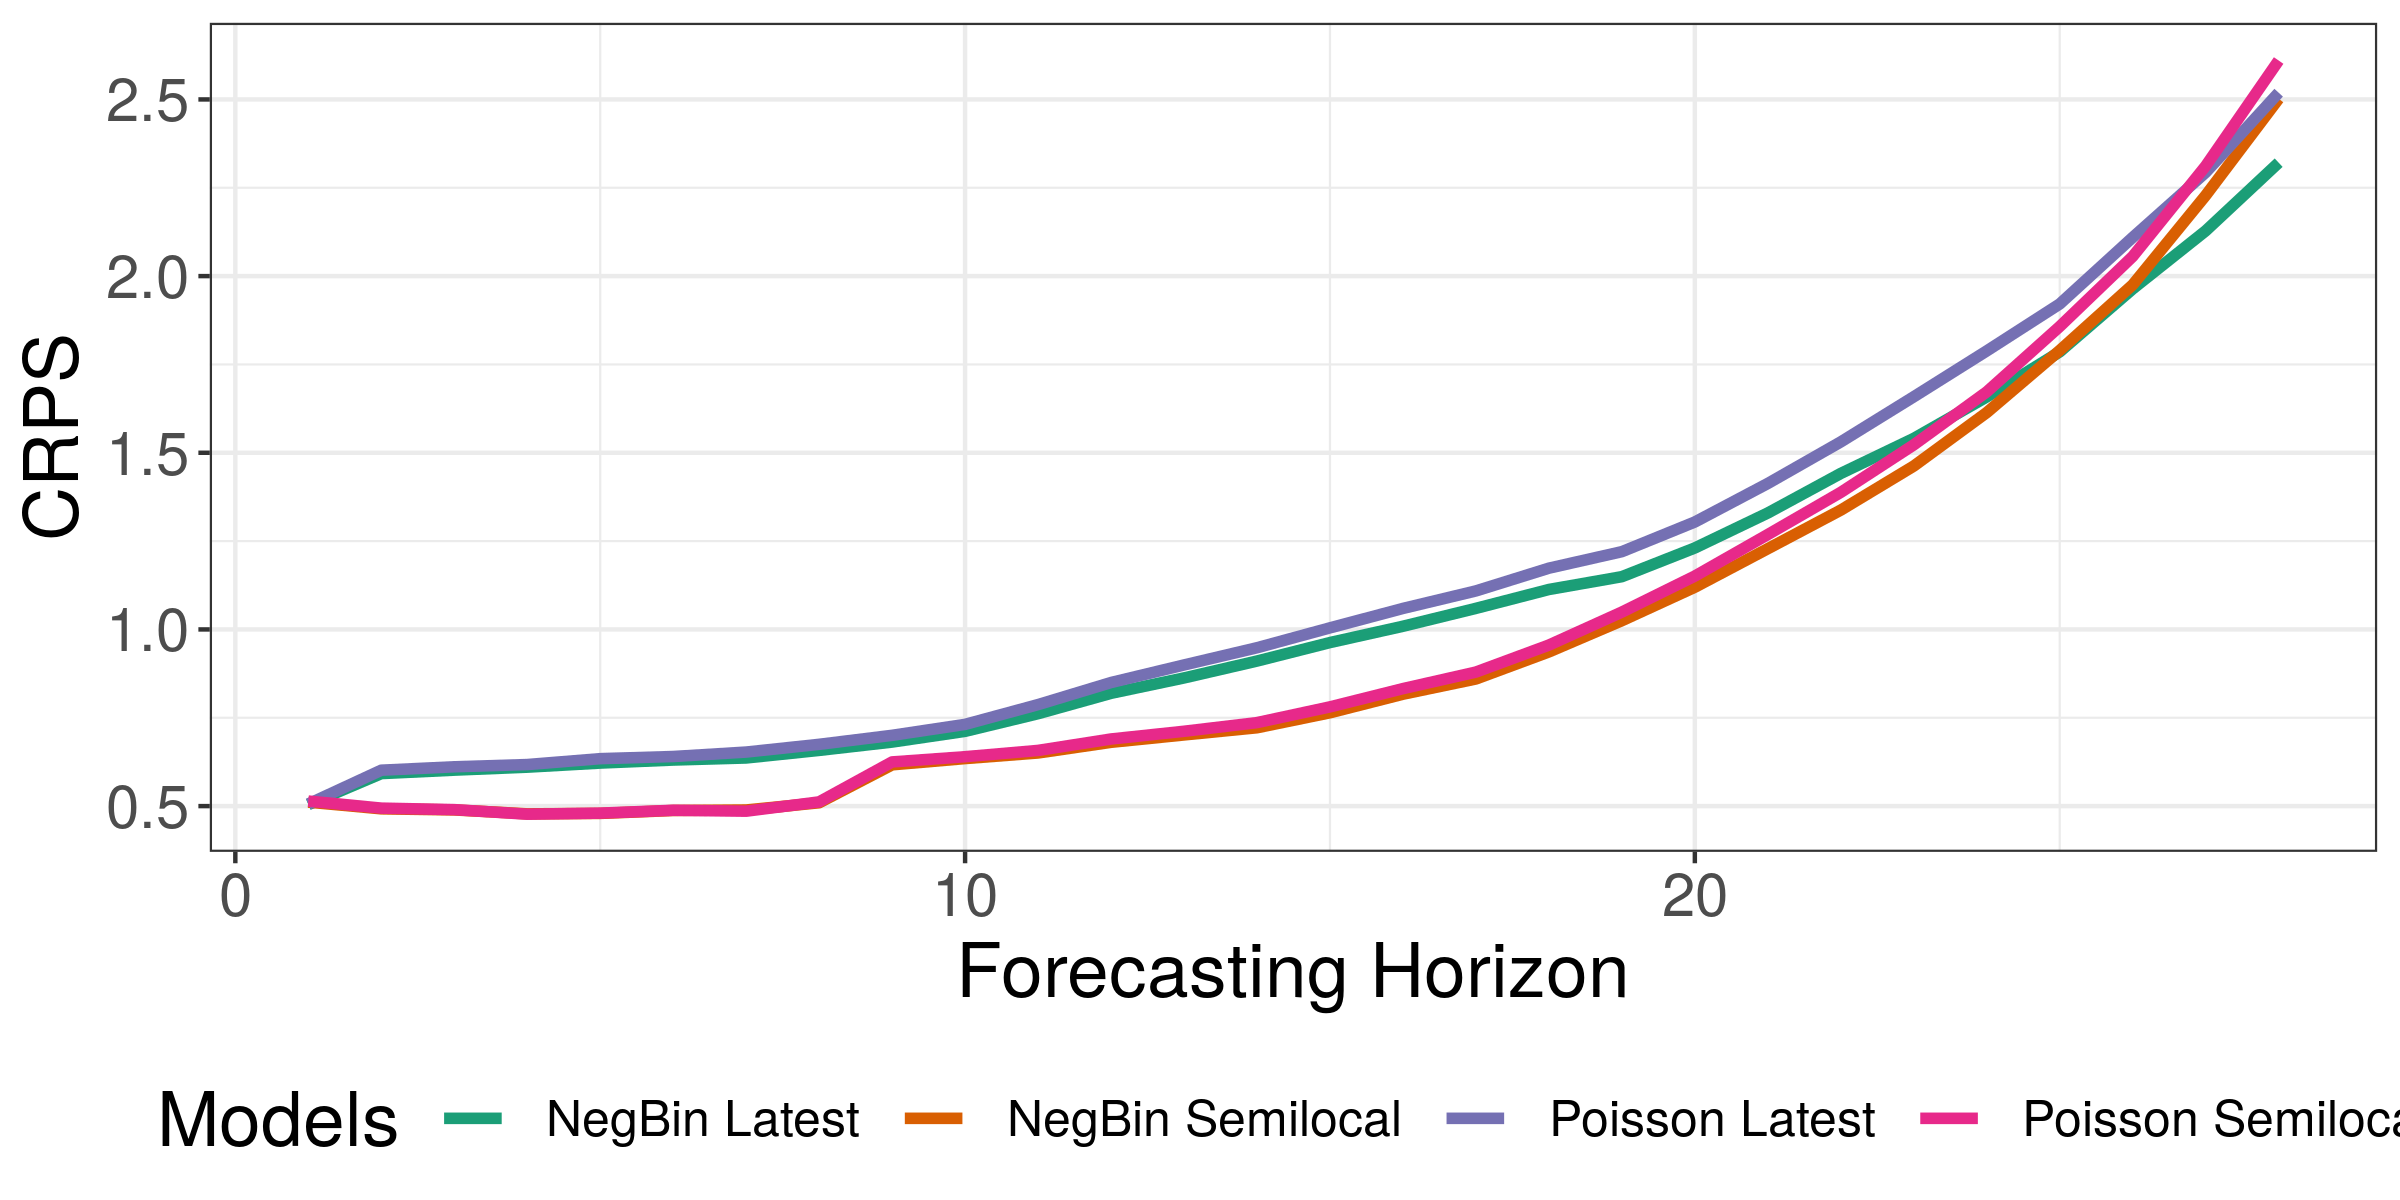
\includegraphics[width=\linewidth]{../output/Butembo_crps.png}  
  \caption{Contineously Ranked Probability Score}
  \label{Butembo_scores_1}
\end{subfigure}
\begin{subfigure}{0.5\textwidth}
  \centering
  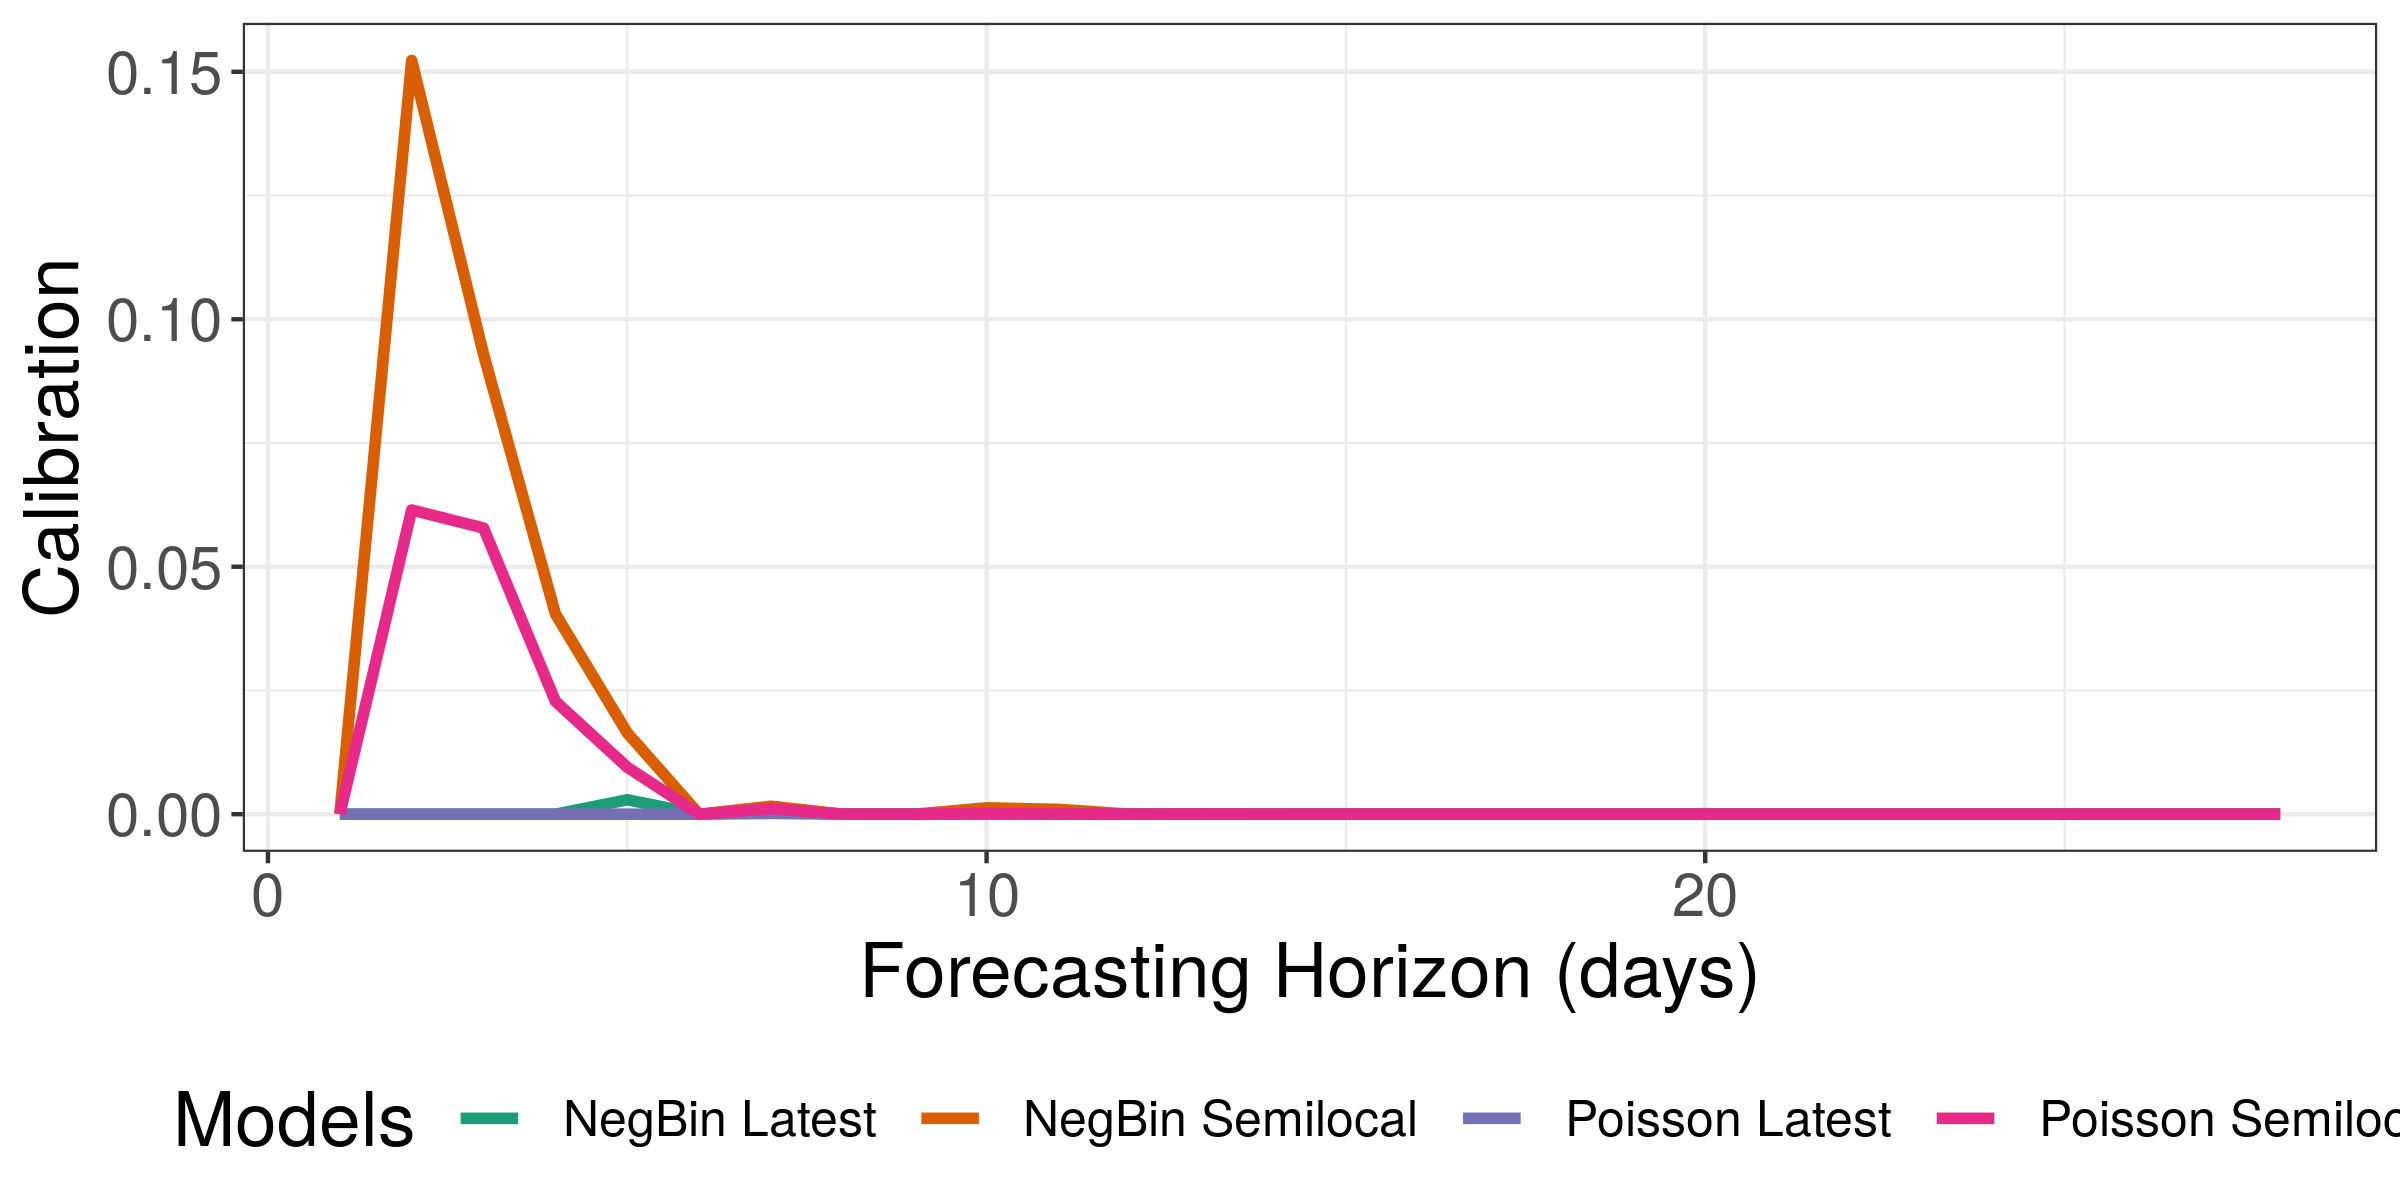
\includegraphics[width=\linewidth]{../output/Butembo_calibration.png}  
  \caption{Calibration p-value}
  \label{Butembo_scores_2}
\end{subfigure}

\begin{subfigure}{0.5\textwidth}
  \centering
  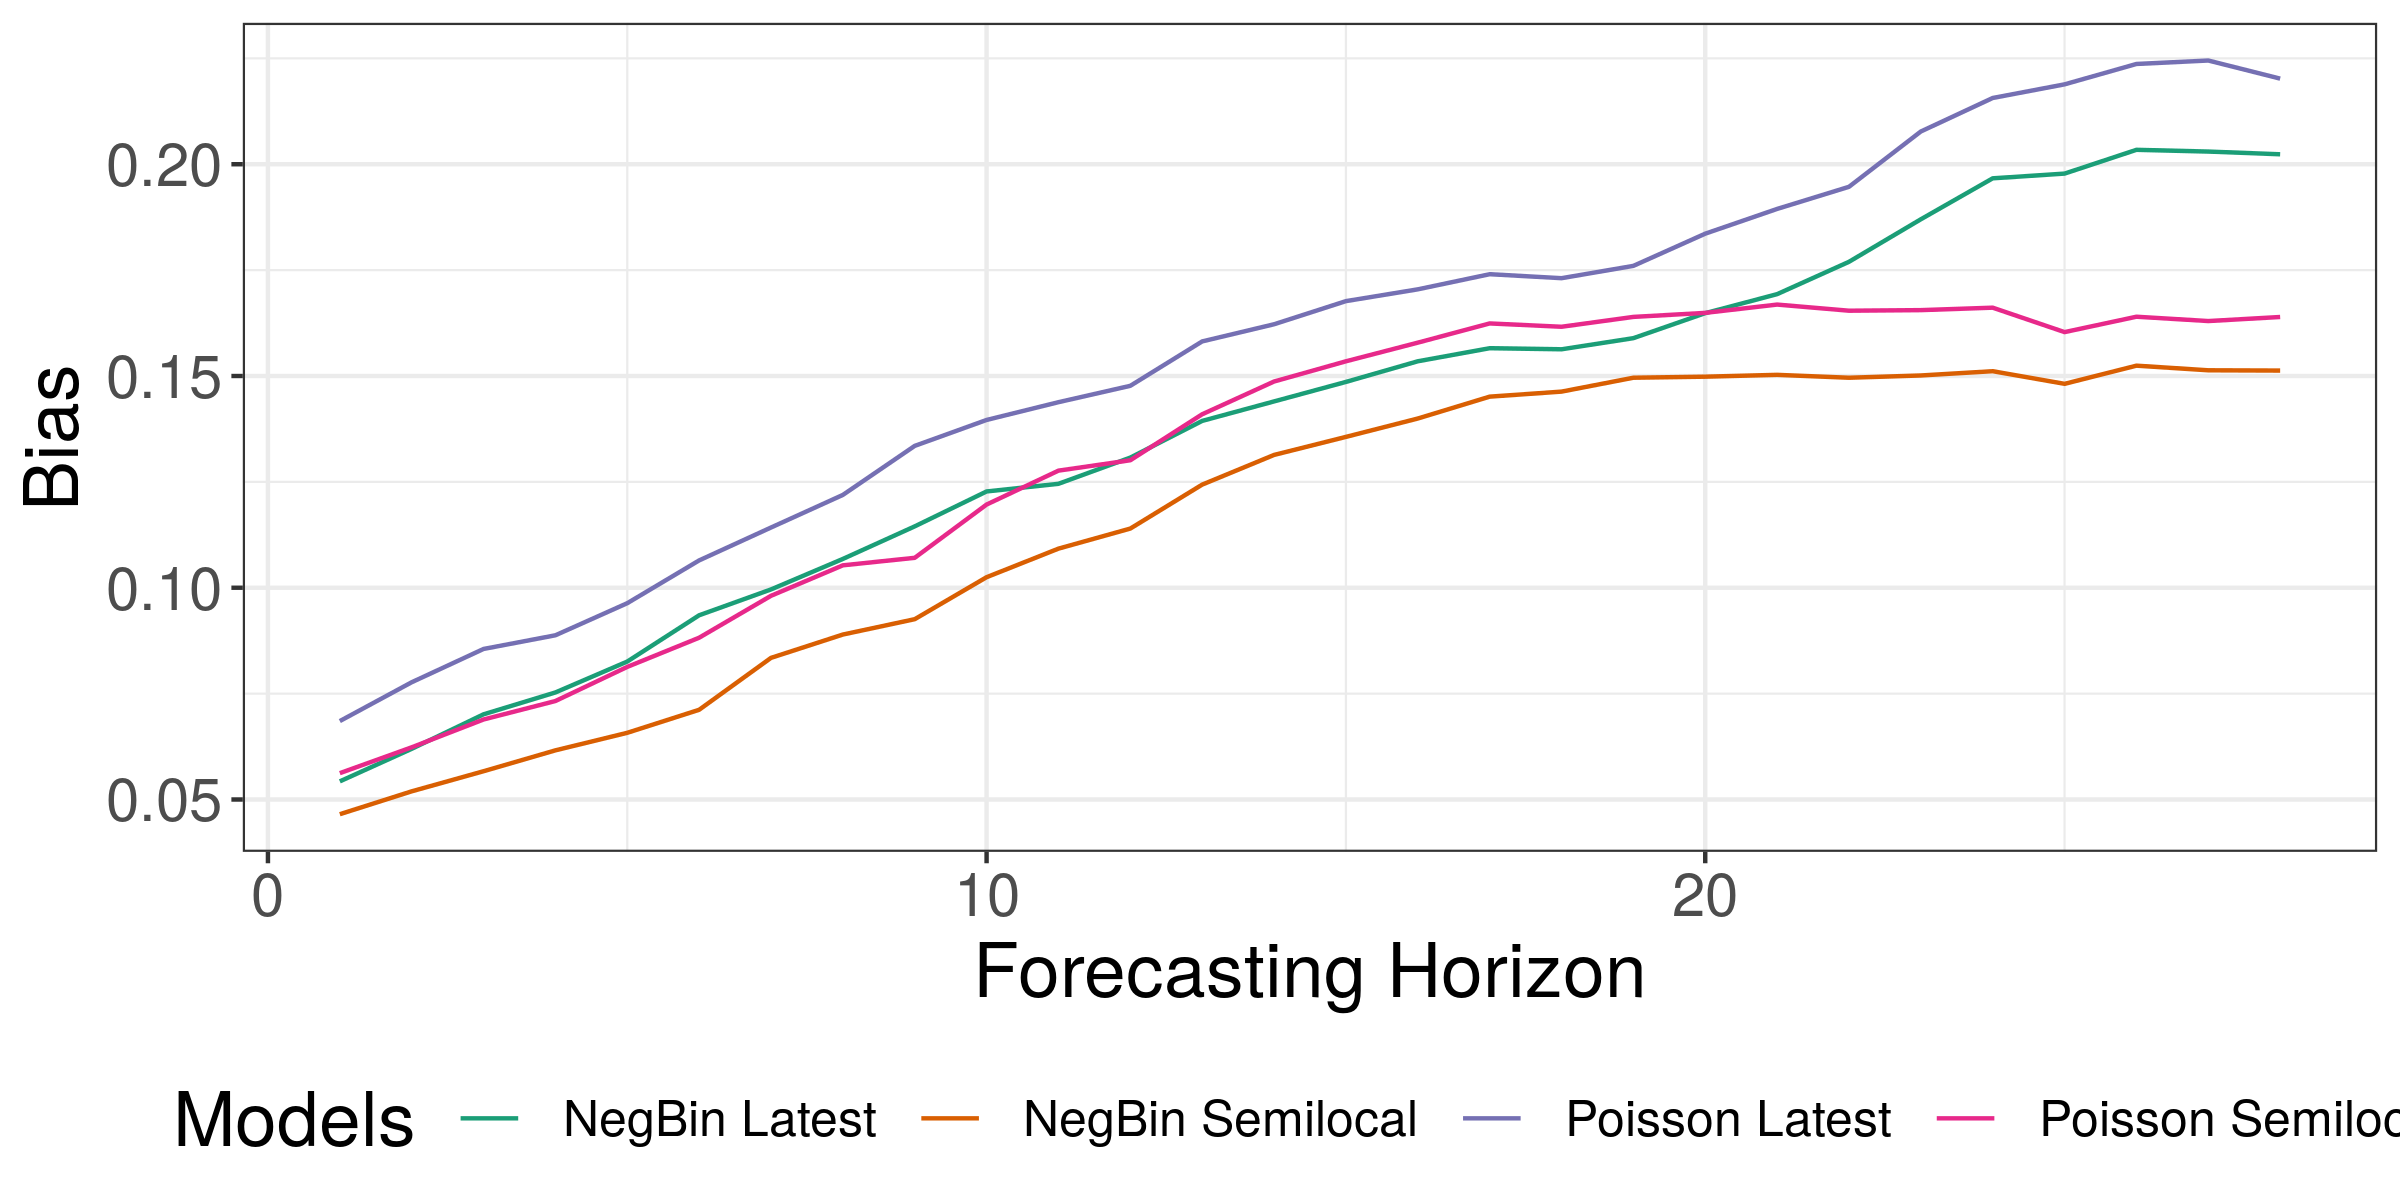
\includegraphics[width=\linewidth]{../output/Butembo_bias.png}  
  \caption{Bias}
  \label{fig:Butembo_scores_3}
\end{subfigure}
\begin{subfigure}{0.5\textwidth}
  \centering
  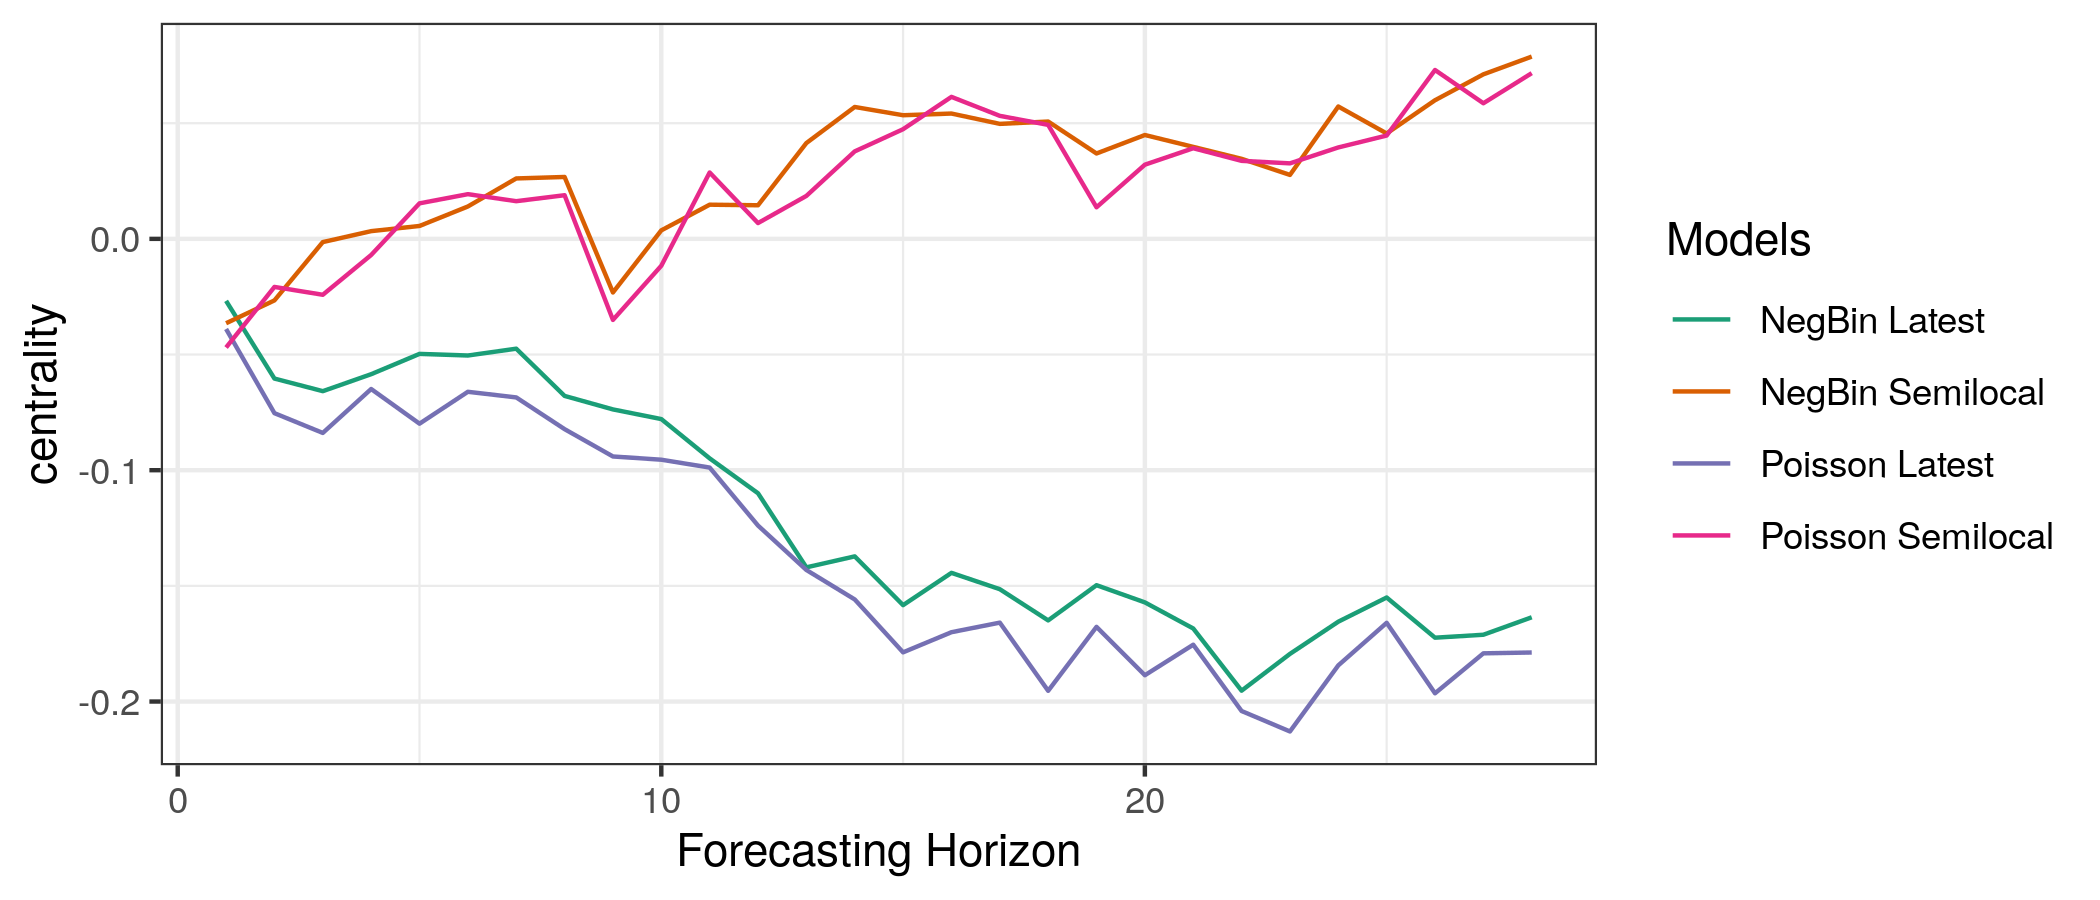
\includegraphics[width=\linewidth]{../output/Butembo_centrality.png}  
  \caption{Centrality of PIT values}
  \label{fig:Butembo_scores_4}
\end{subfigure}
  \caption{Scores for Butembo as a function of the forecasting horizon.}

  \label{fig:nat_scores}
\end{figure}
 \section{ Mabalako }\begin{figure}[H]\begin{subfigure}{\textwidth}  \centering  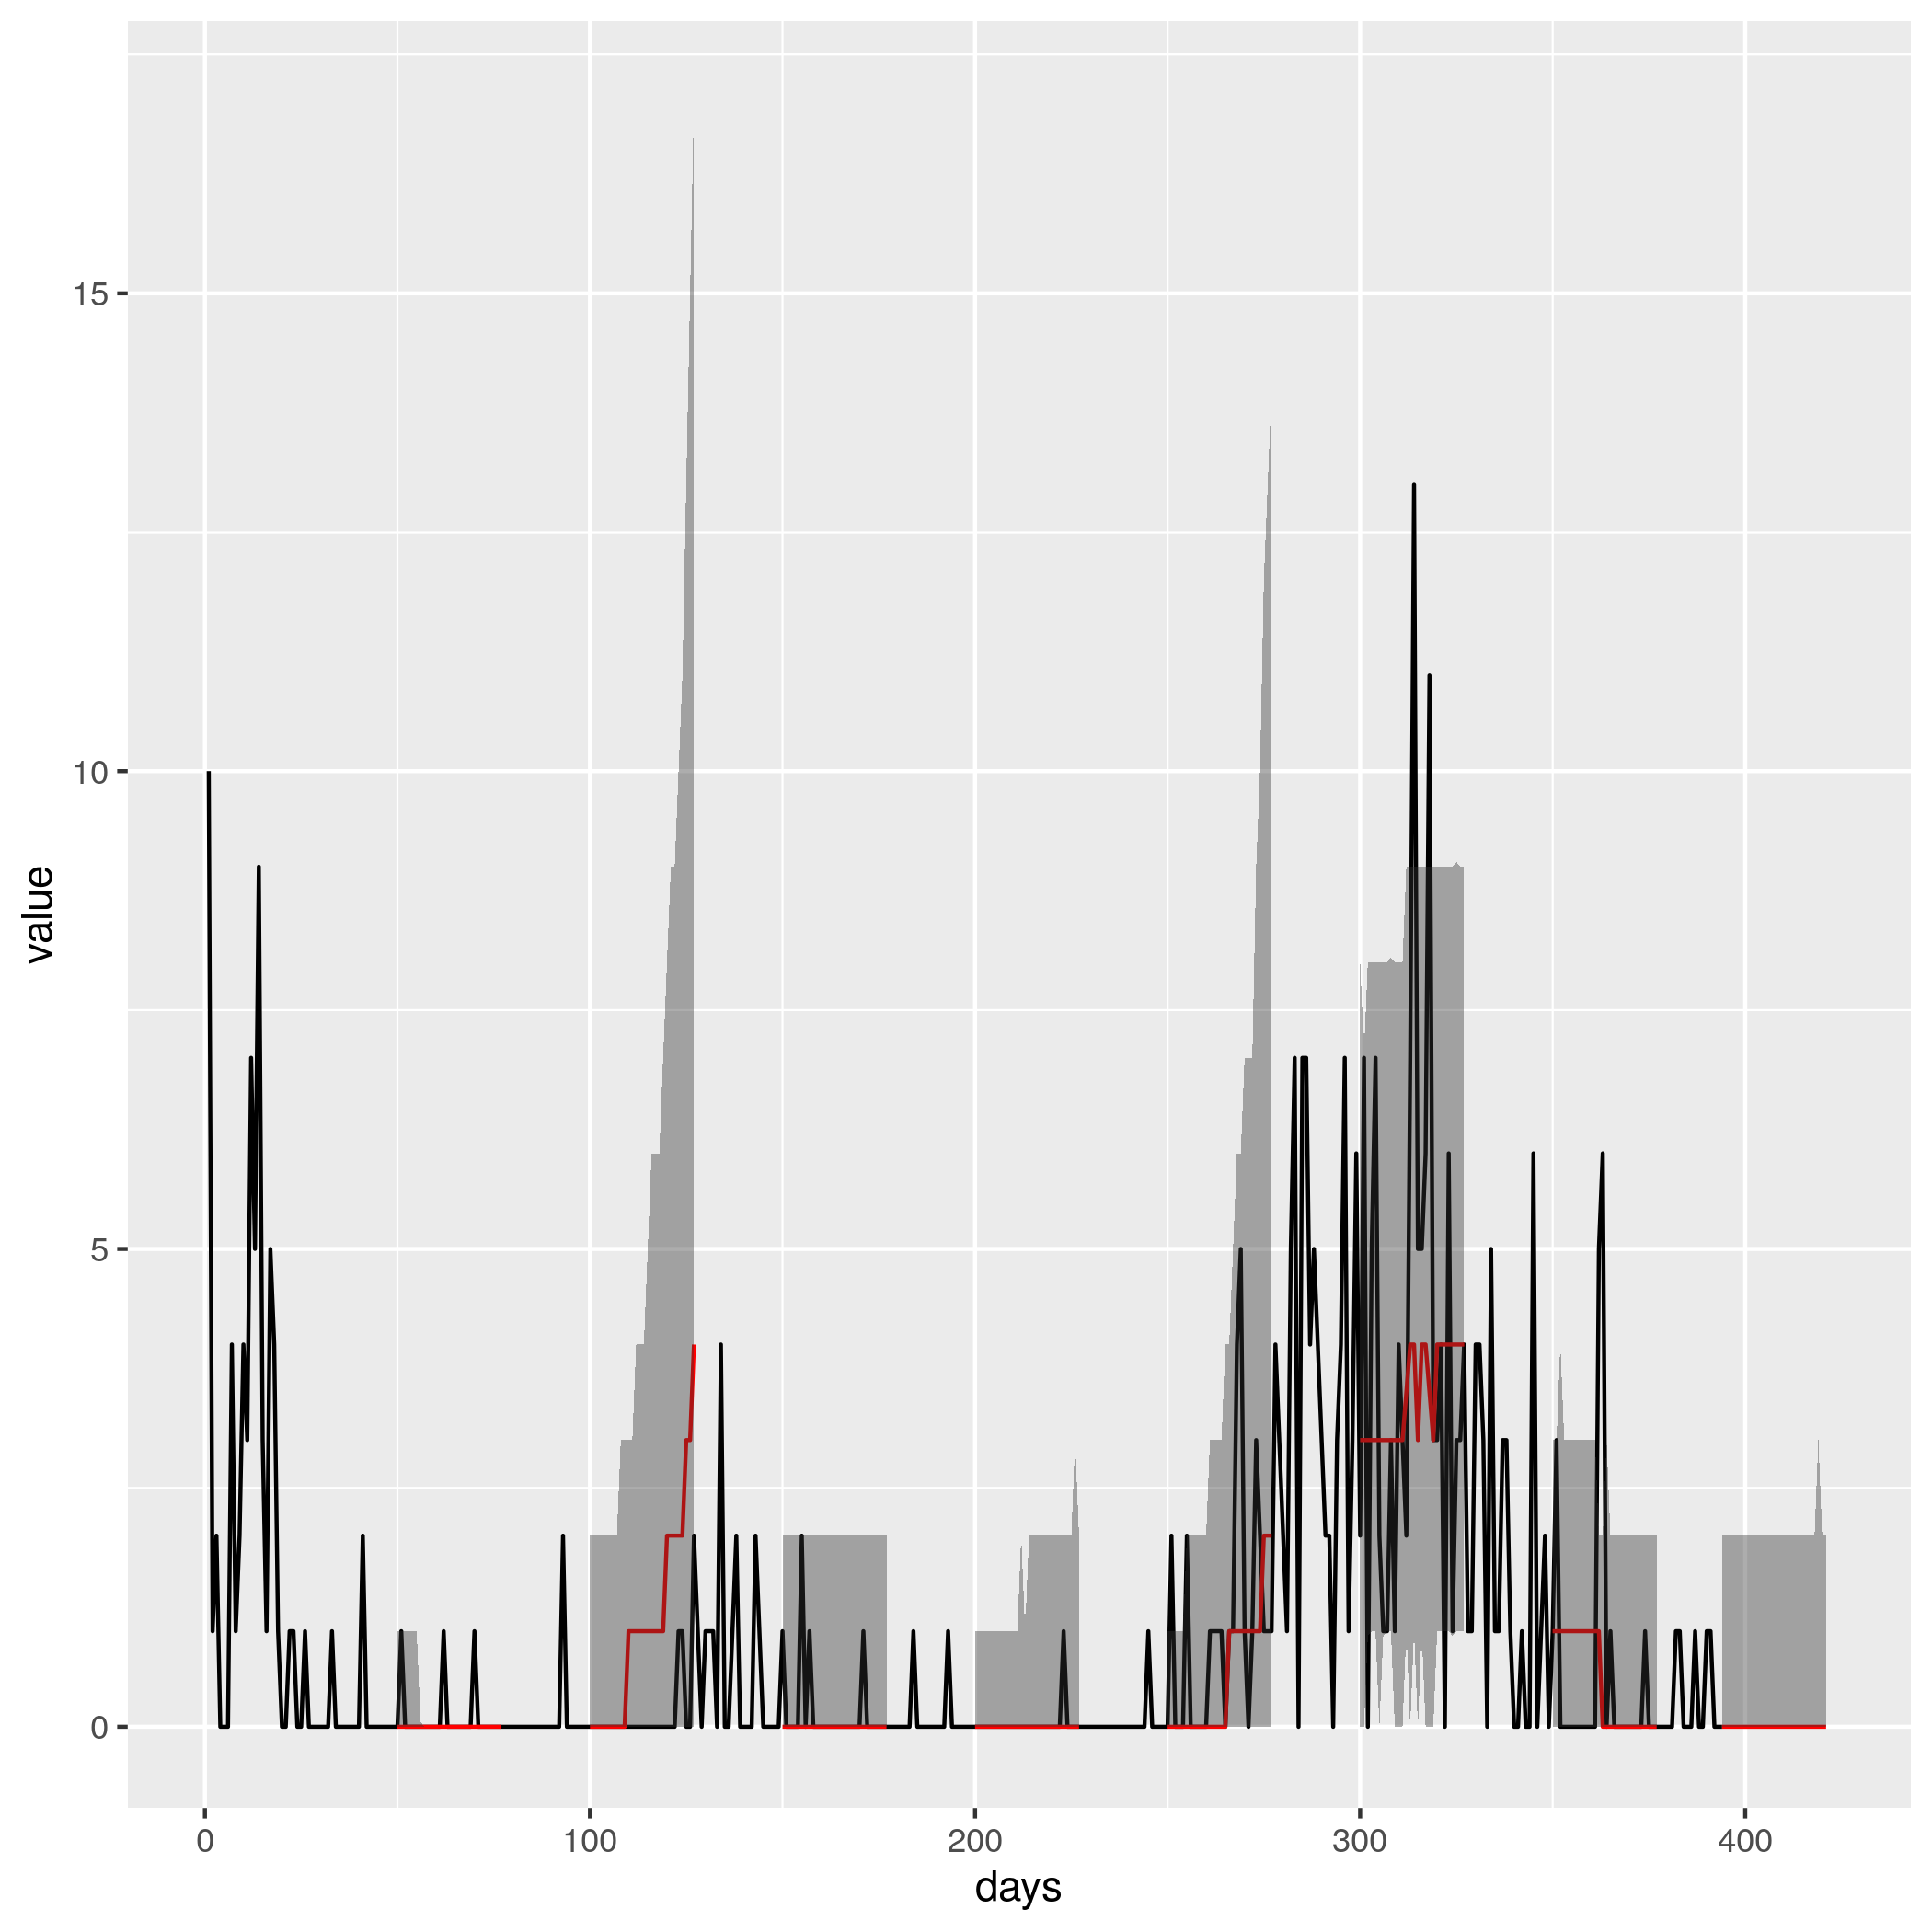
\includegraphics[width=0.9\linewidth, height=7cm]{../output/Mabalako_predictions.png}  \caption{Forecasted and predicted incidence for the best fitting model}\end{subfigure}

\begin{subfigure}{\textwidth}  \centering  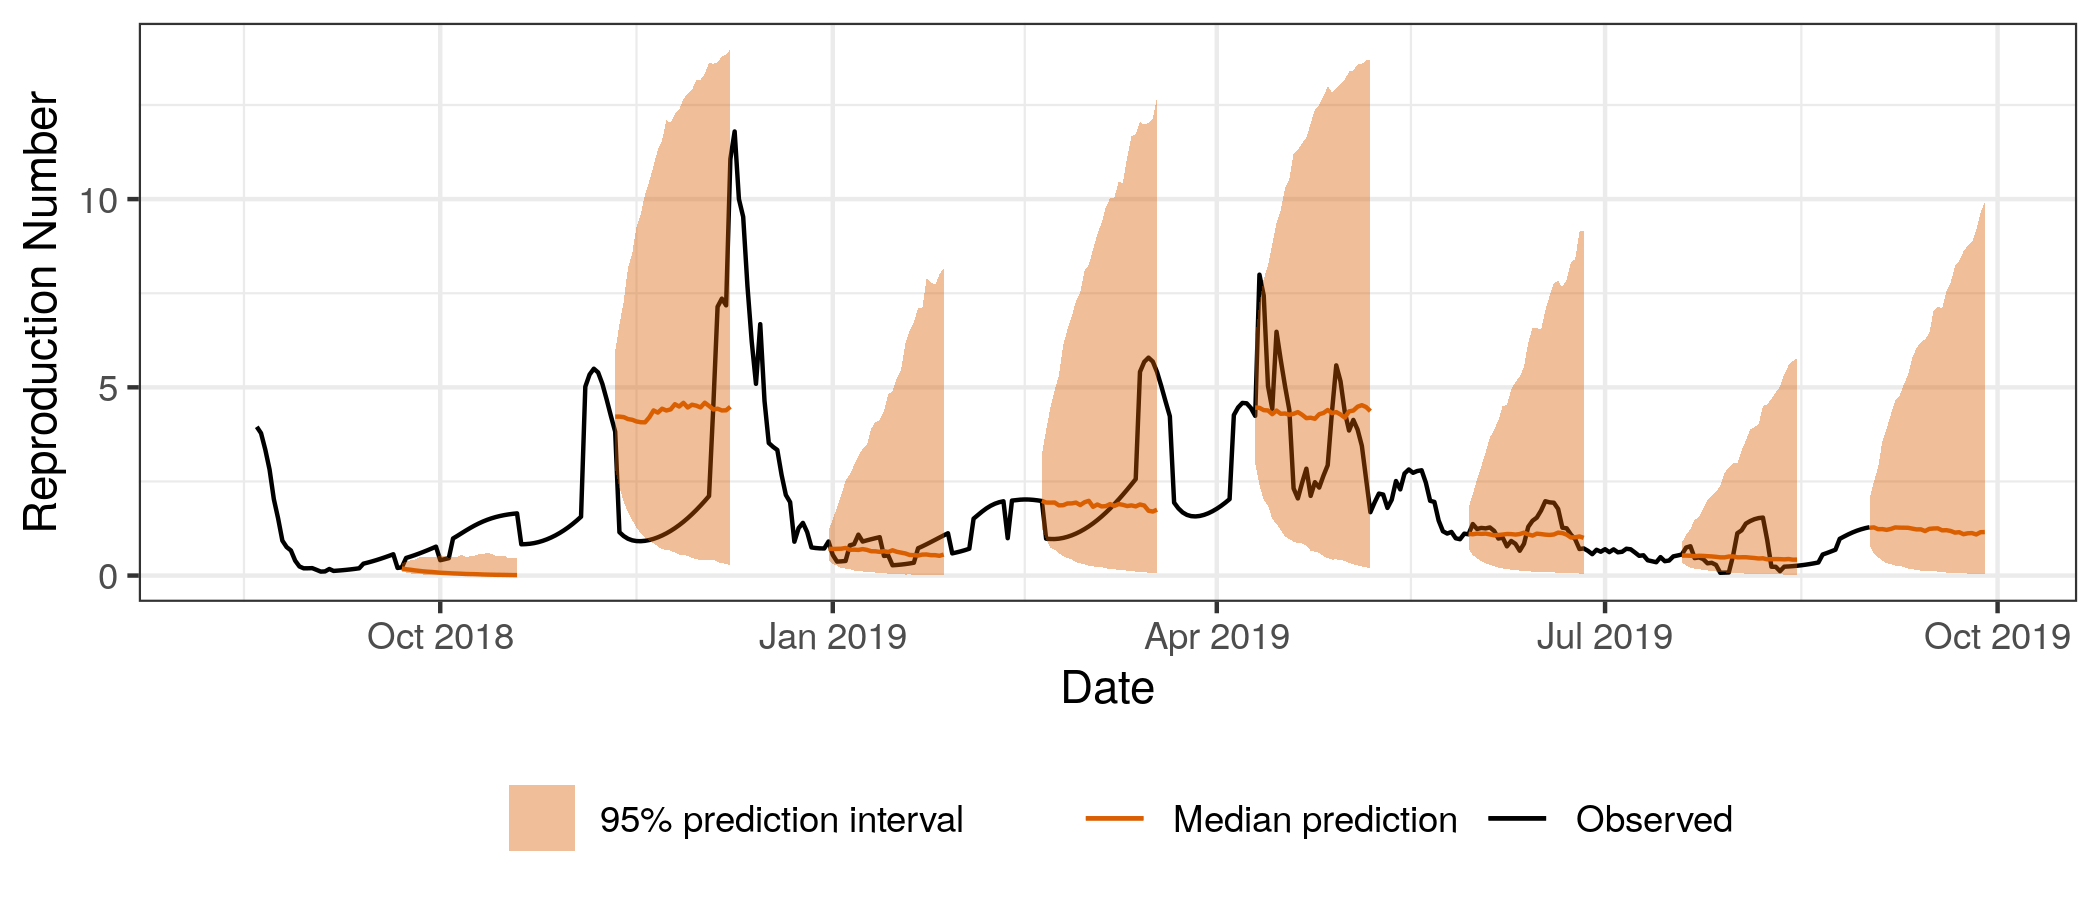
\includegraphics[width=0.9\linewidth, height=7cm]{../output/Mabalako_Rs.png}  \caption{Forecasted and predicted repreoduction numbers for the best fitting model}\end{subfigure}  \caption{Median forecast with 95 \% prediction intervals and observed values for incidence and reproduction number for the best fitting model for Mabalako.}\end{figure}

\begin{figure}[H]
\begin{subfigure}{0.5\textwidth}
  \centering
  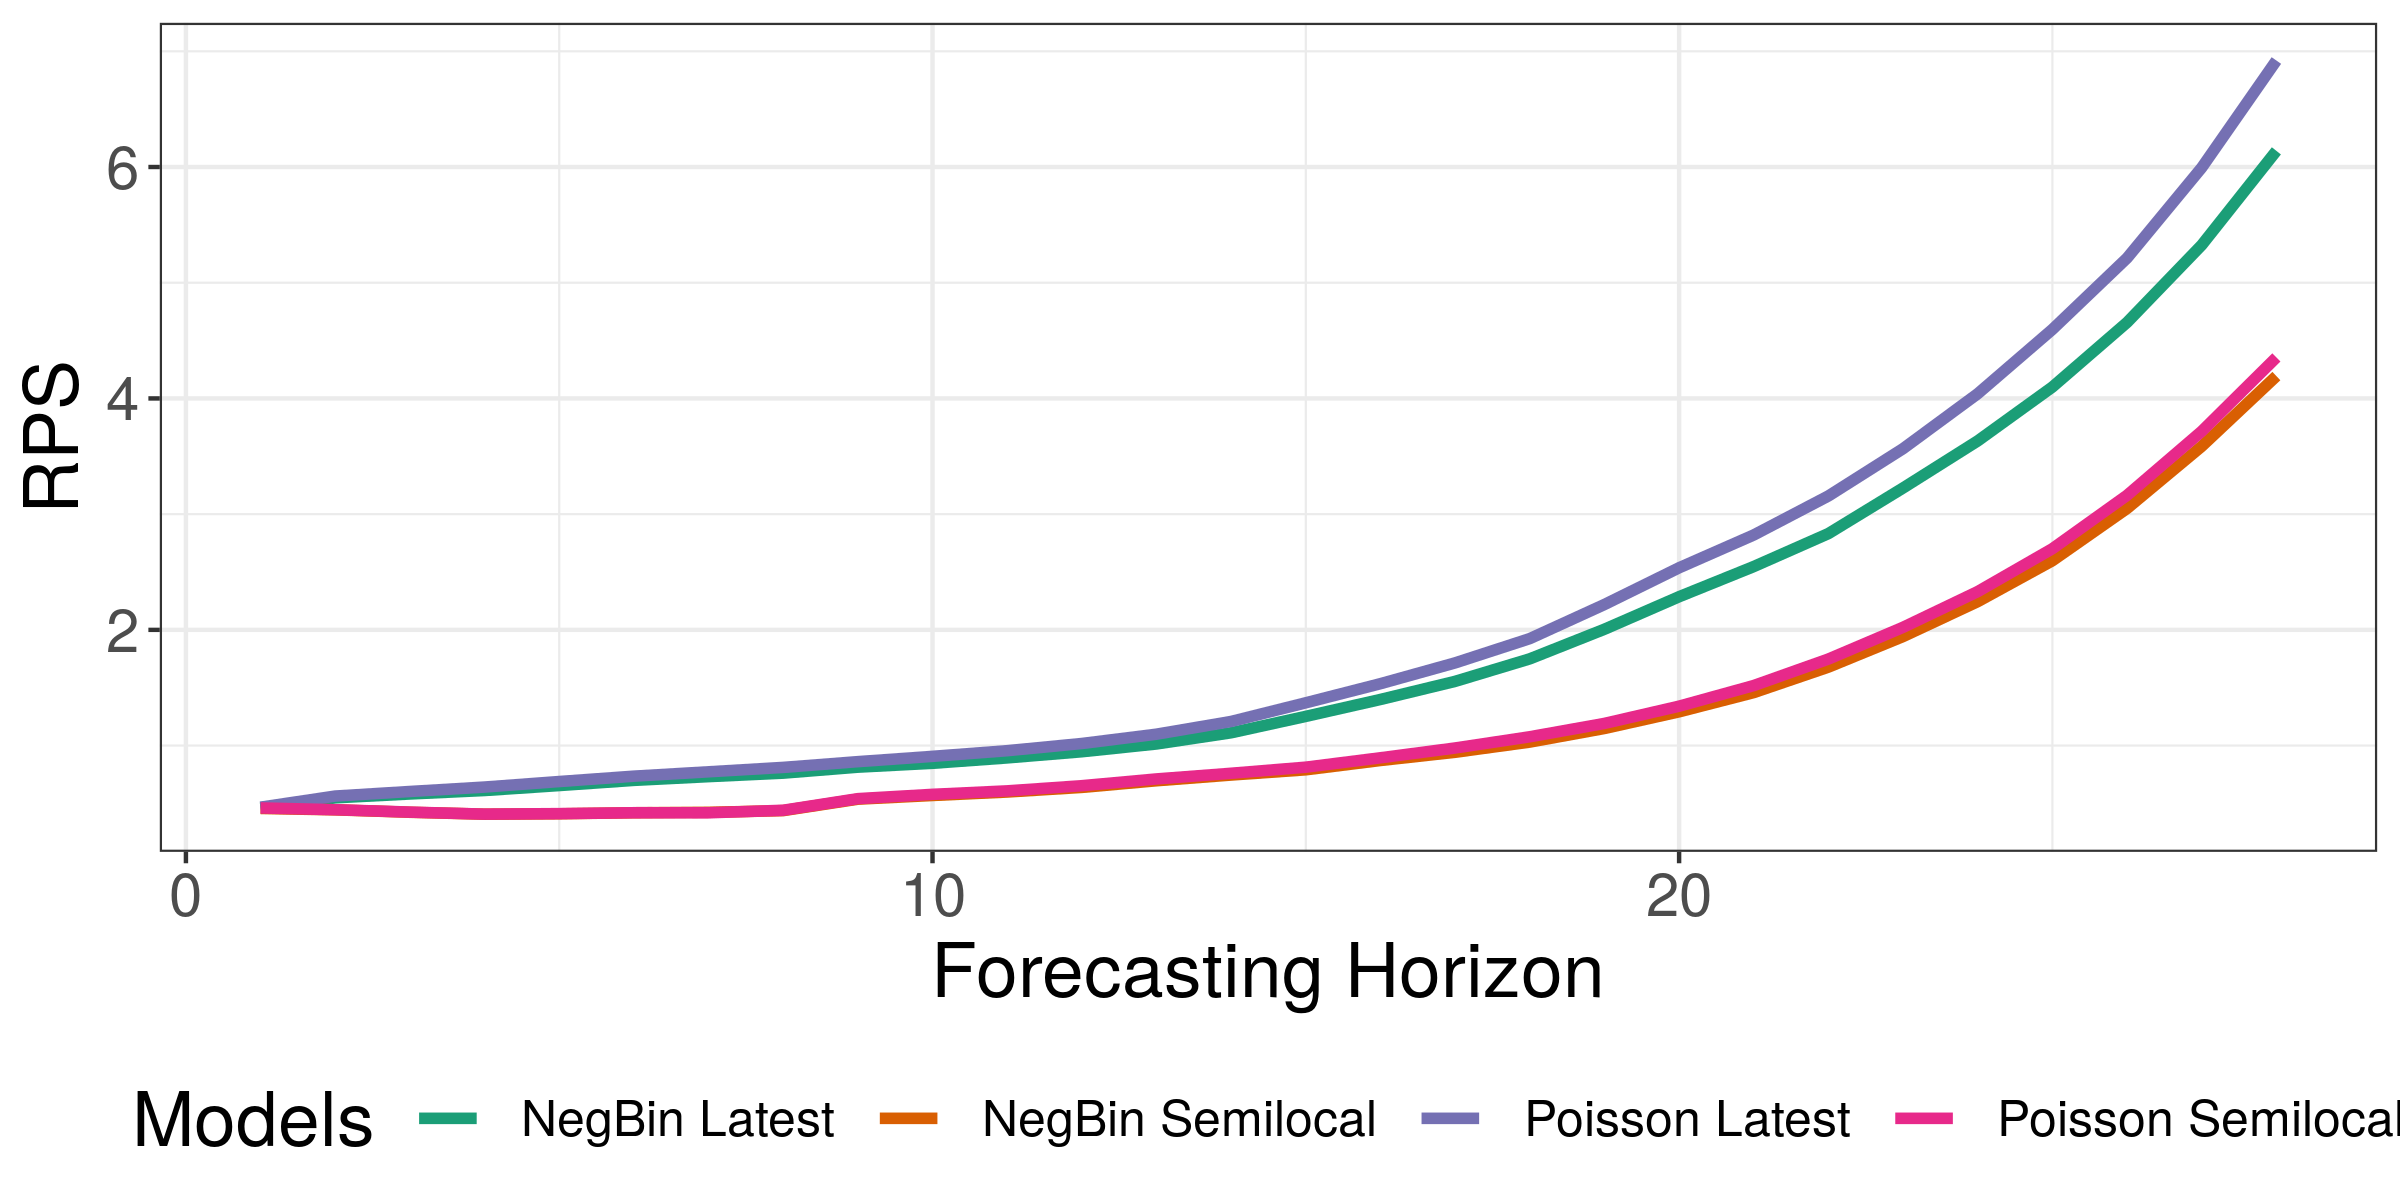
\includegraphics[width=\linewidth]{../output/Mabalako_crps.png}  
  \caption{Contineously Ranked Probability Score}
  \label{Mabalako_scores_1}
\end{subfigure}
\begin{subfigure}{0.5\textwidth}
  \centering
  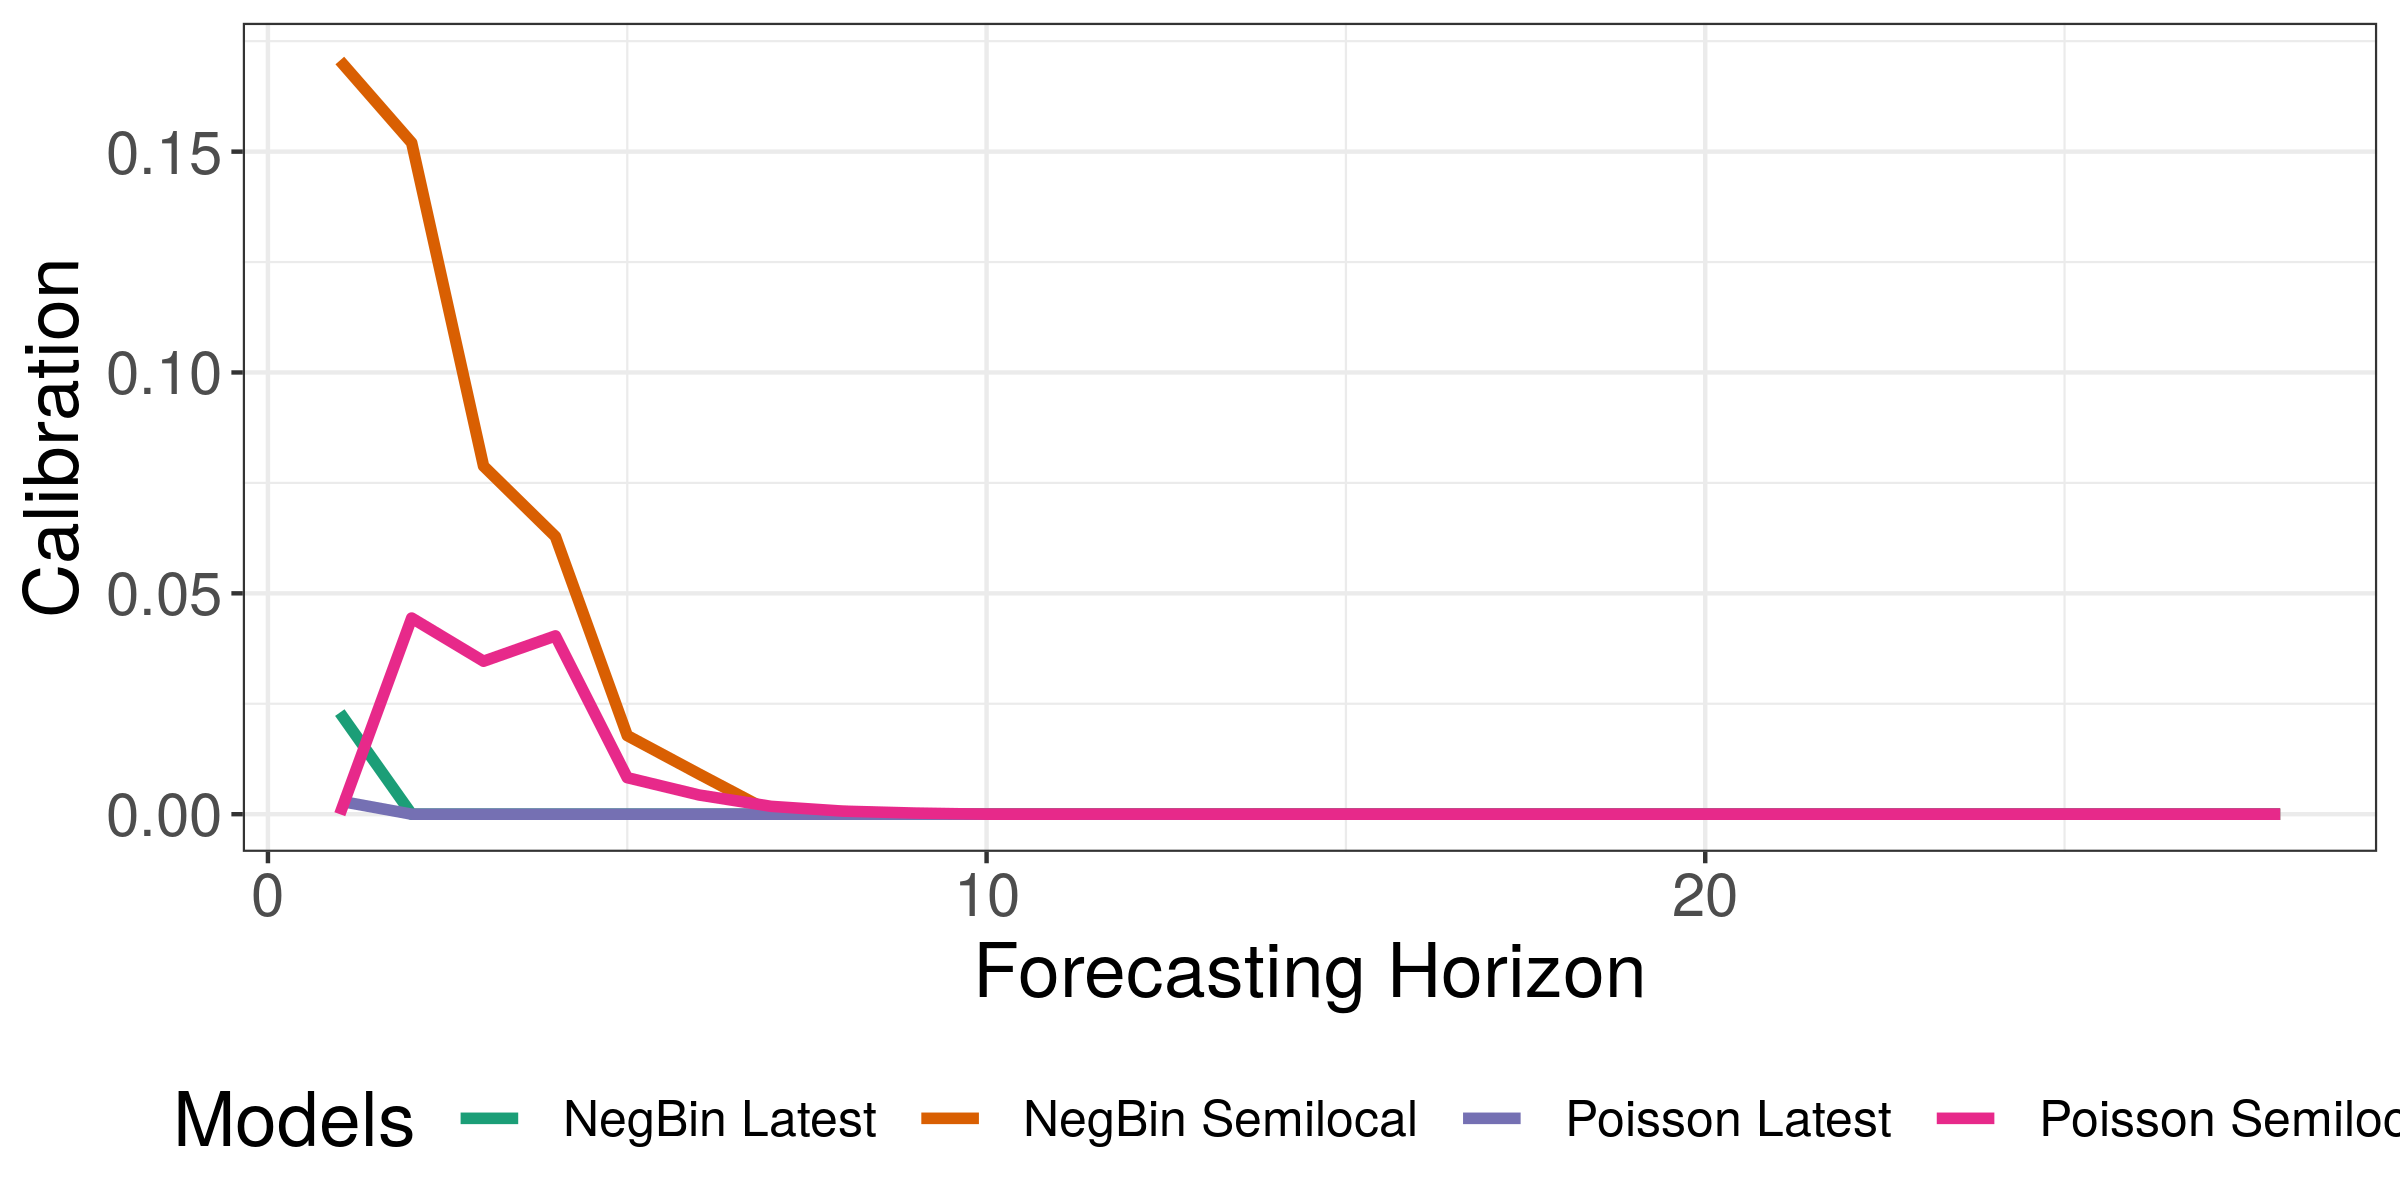
\includegraphics[width=\linewidth]{../output/Mabalako_calibration.png}  
  \caption{Calibration p-value}
  \label{Mabalako_scores_2}
\end{subfigure}

\begin{subfigure}{0.5\textwidth}
  \centering
  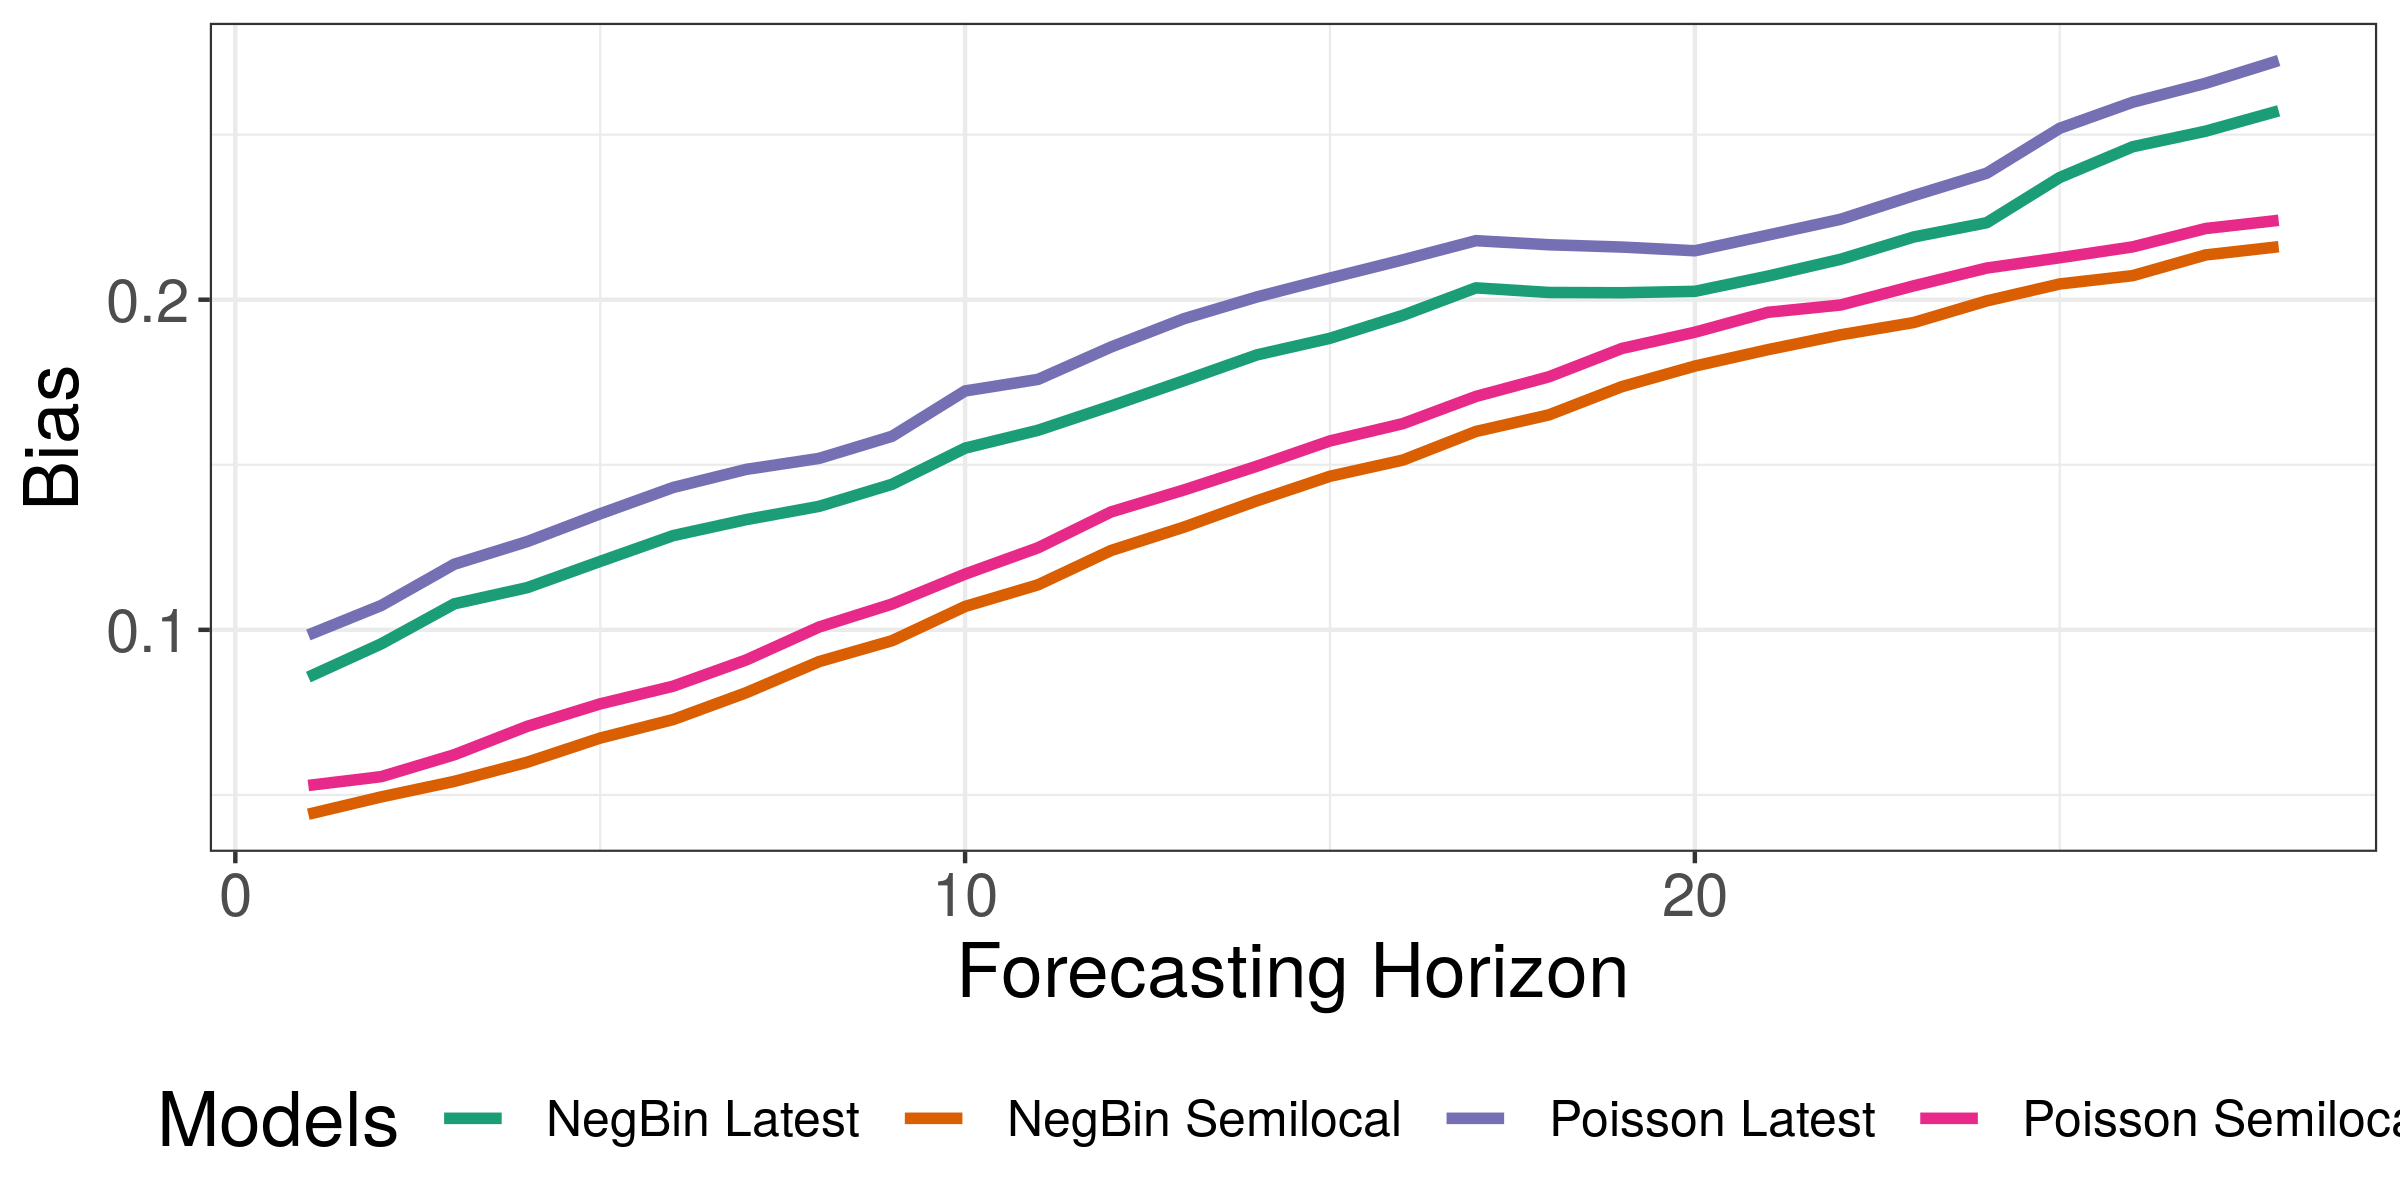
\includegraphics[width=\linewidth]{../output/Mabalako_bias.png}  
  \caption{Bias}
  \label{fig:Mabalako_scores_3}
\end{subfigure}
\begin{subfigure}{0.5\textwidth}
  \centering
  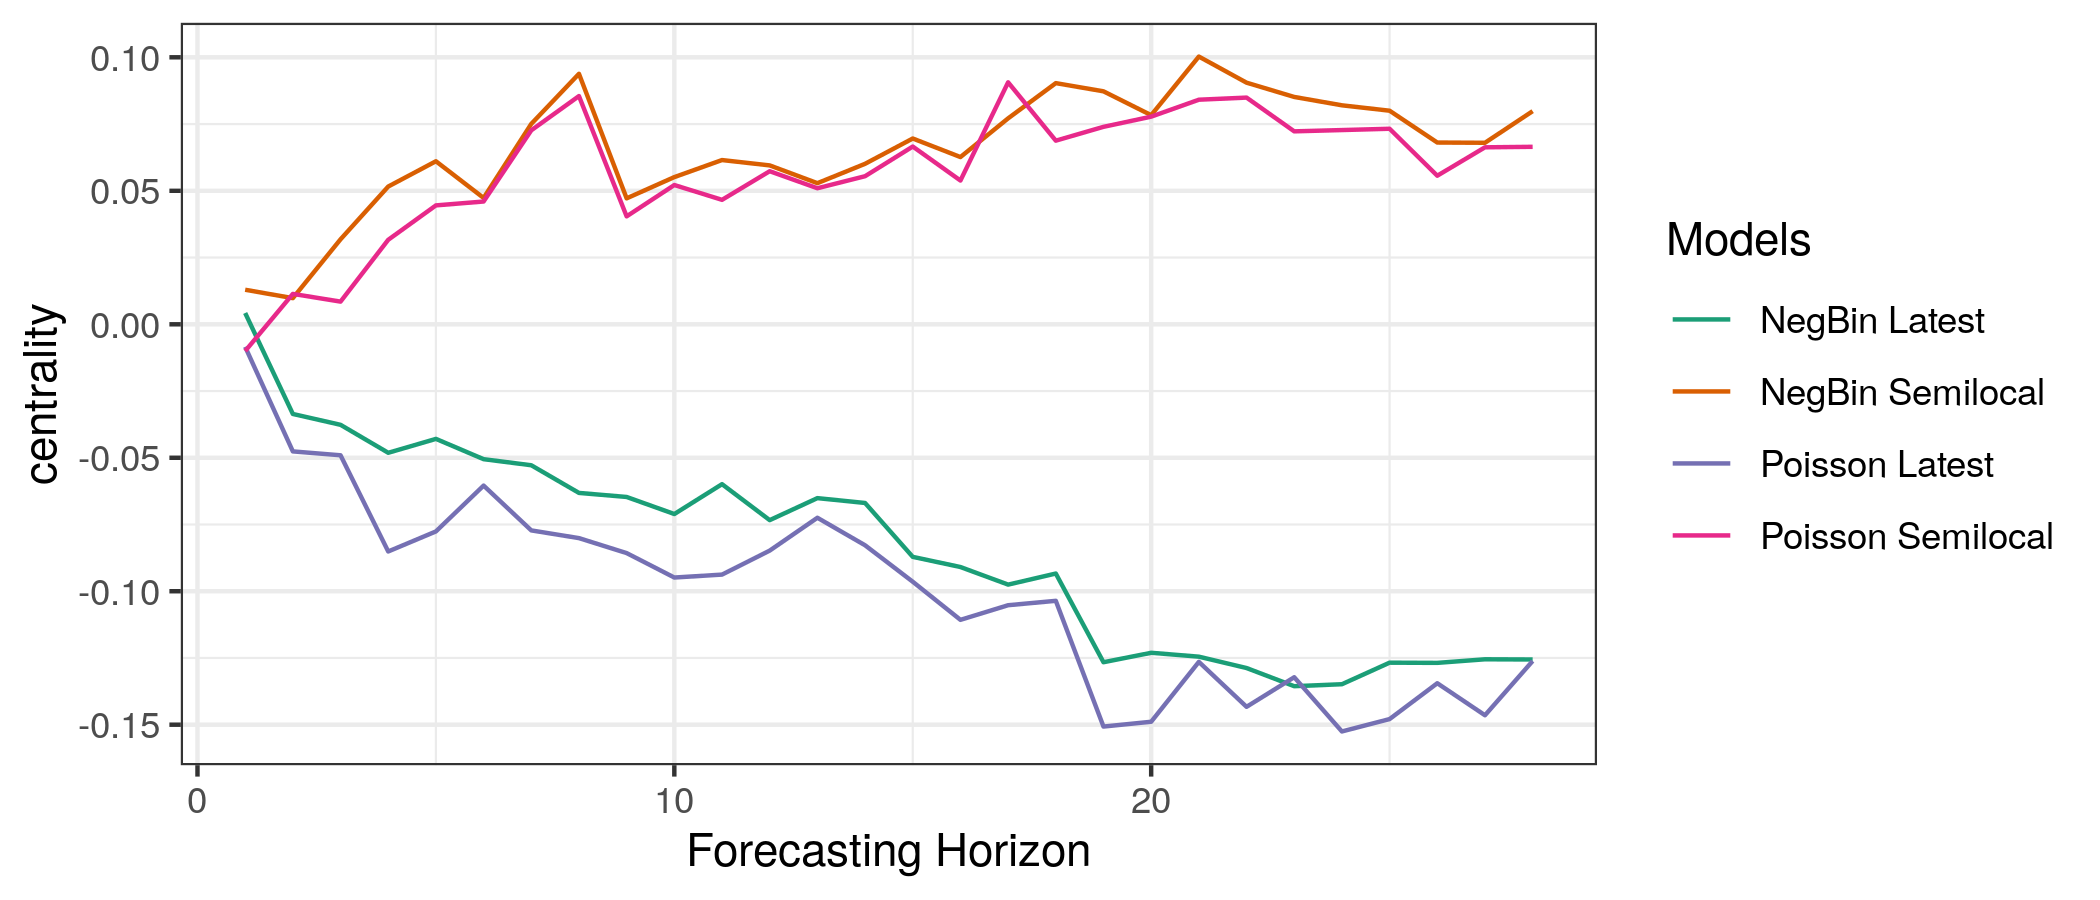
\includegraphics[width=\linewidth]{../output/Mabalako_centrality.png}  
  \caption{Centrality of PIT values}
  \label{fig:Mabalako_scores_4}
\end{subfigure}
  \caption{Scores for Mabalako as a function of the forecasting horizon.}

  \label{fig:nat_scores}
\end{figure}
 \section{ Tchomia }\begin{figure}[H]\begin{subfigure}{\textwidth}  \centering  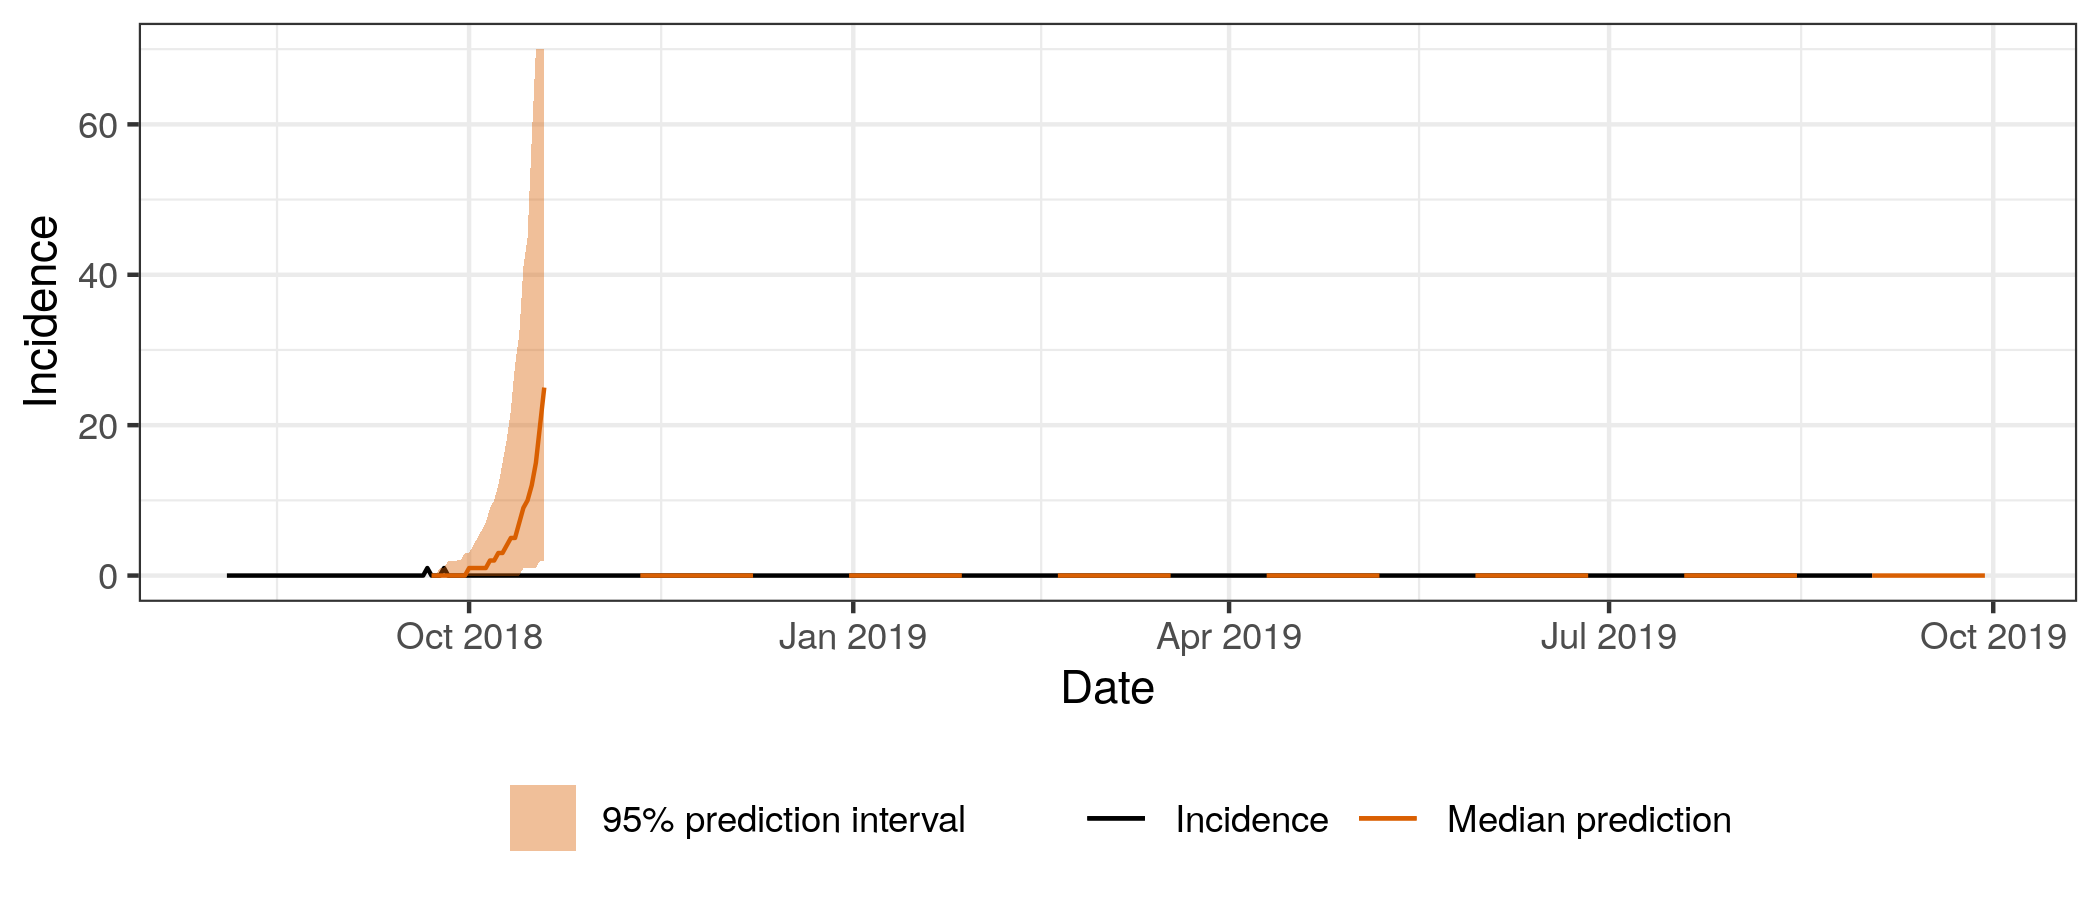
\includegraphics[width=0.9\linewidth, height=7cm]{../output/Tchomia_predictions.png}  \caption{Forecasted and predicted incidence for the best fitting model}\end{subfigure}

\begin{subfigure}{\textwidth}  \centering  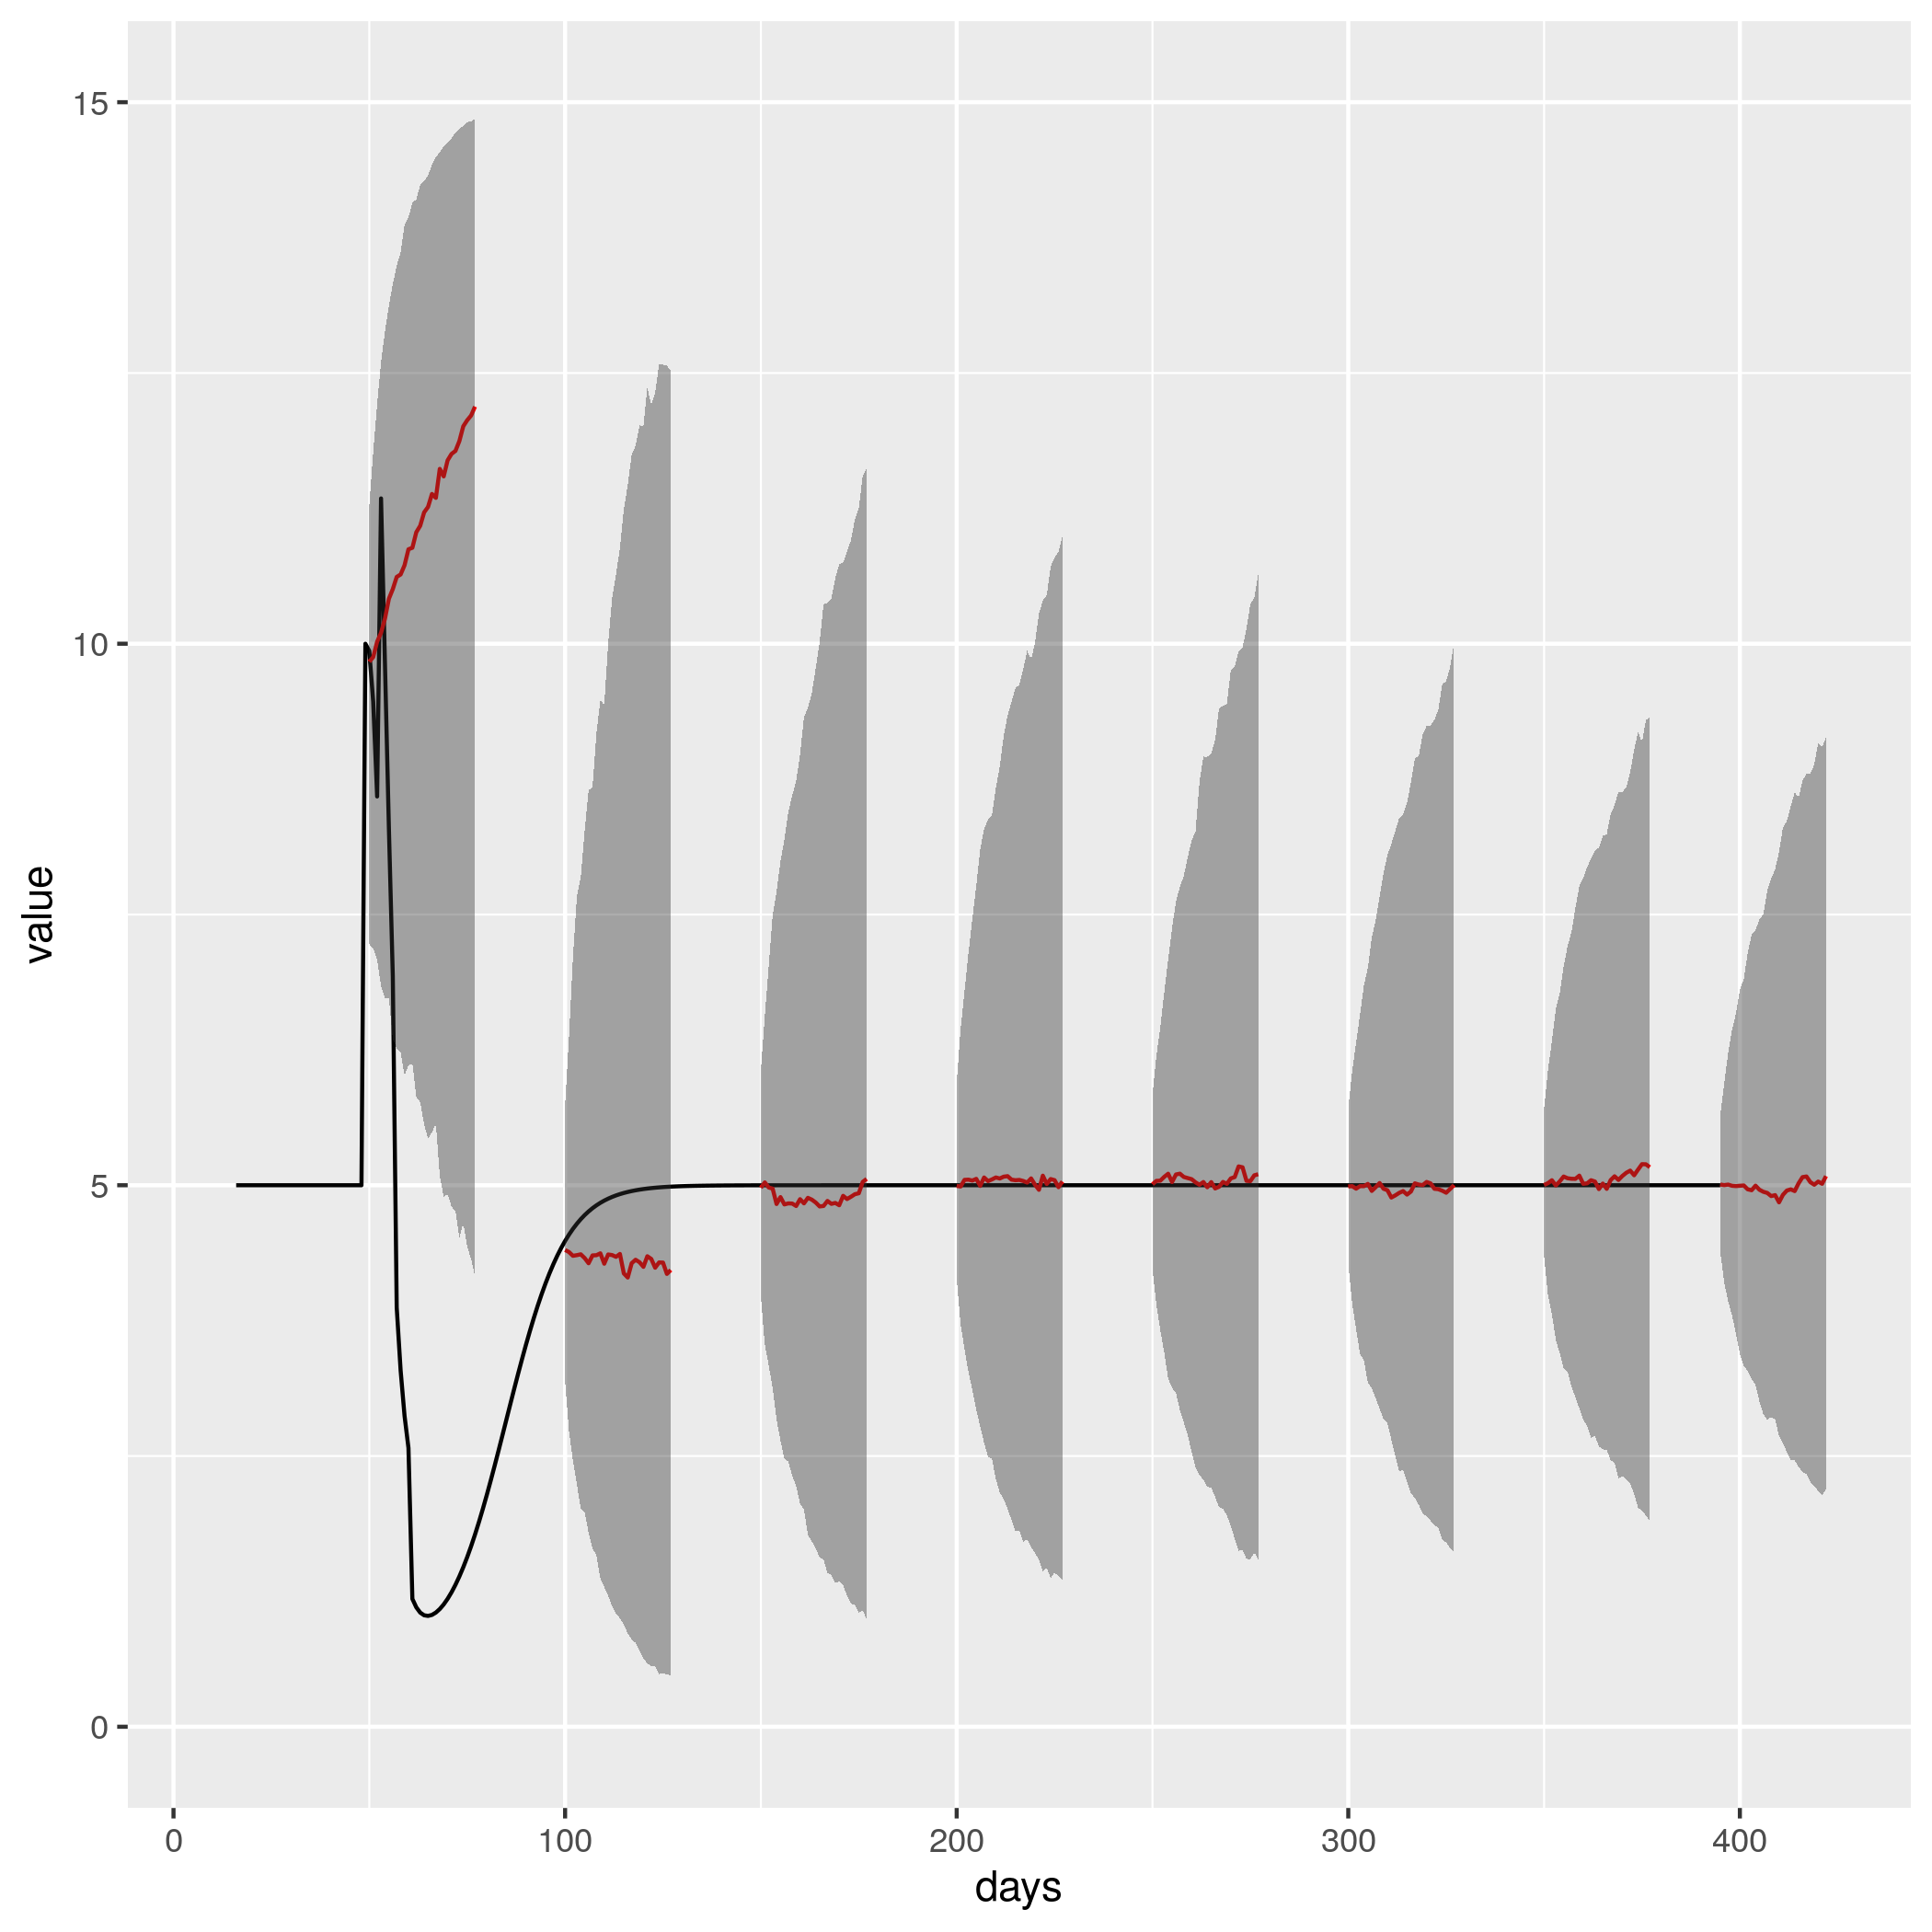
\includegraphics[width=0.9\linewidth, height=7cm]{../output/Tchomia_Rs.png}  \caption{Forecasted and predicted repreoduction numbers for the best fitting model}\end{subfigure}  \caption{Median forecast with 95 \% prediction intervals and observed values for incidence and reproduction number for the best fitting model for Tchomia.}\end{figure}

\begin{figure}[H]
\begin{subfigure}{0.5\textwidth}
  \centering
  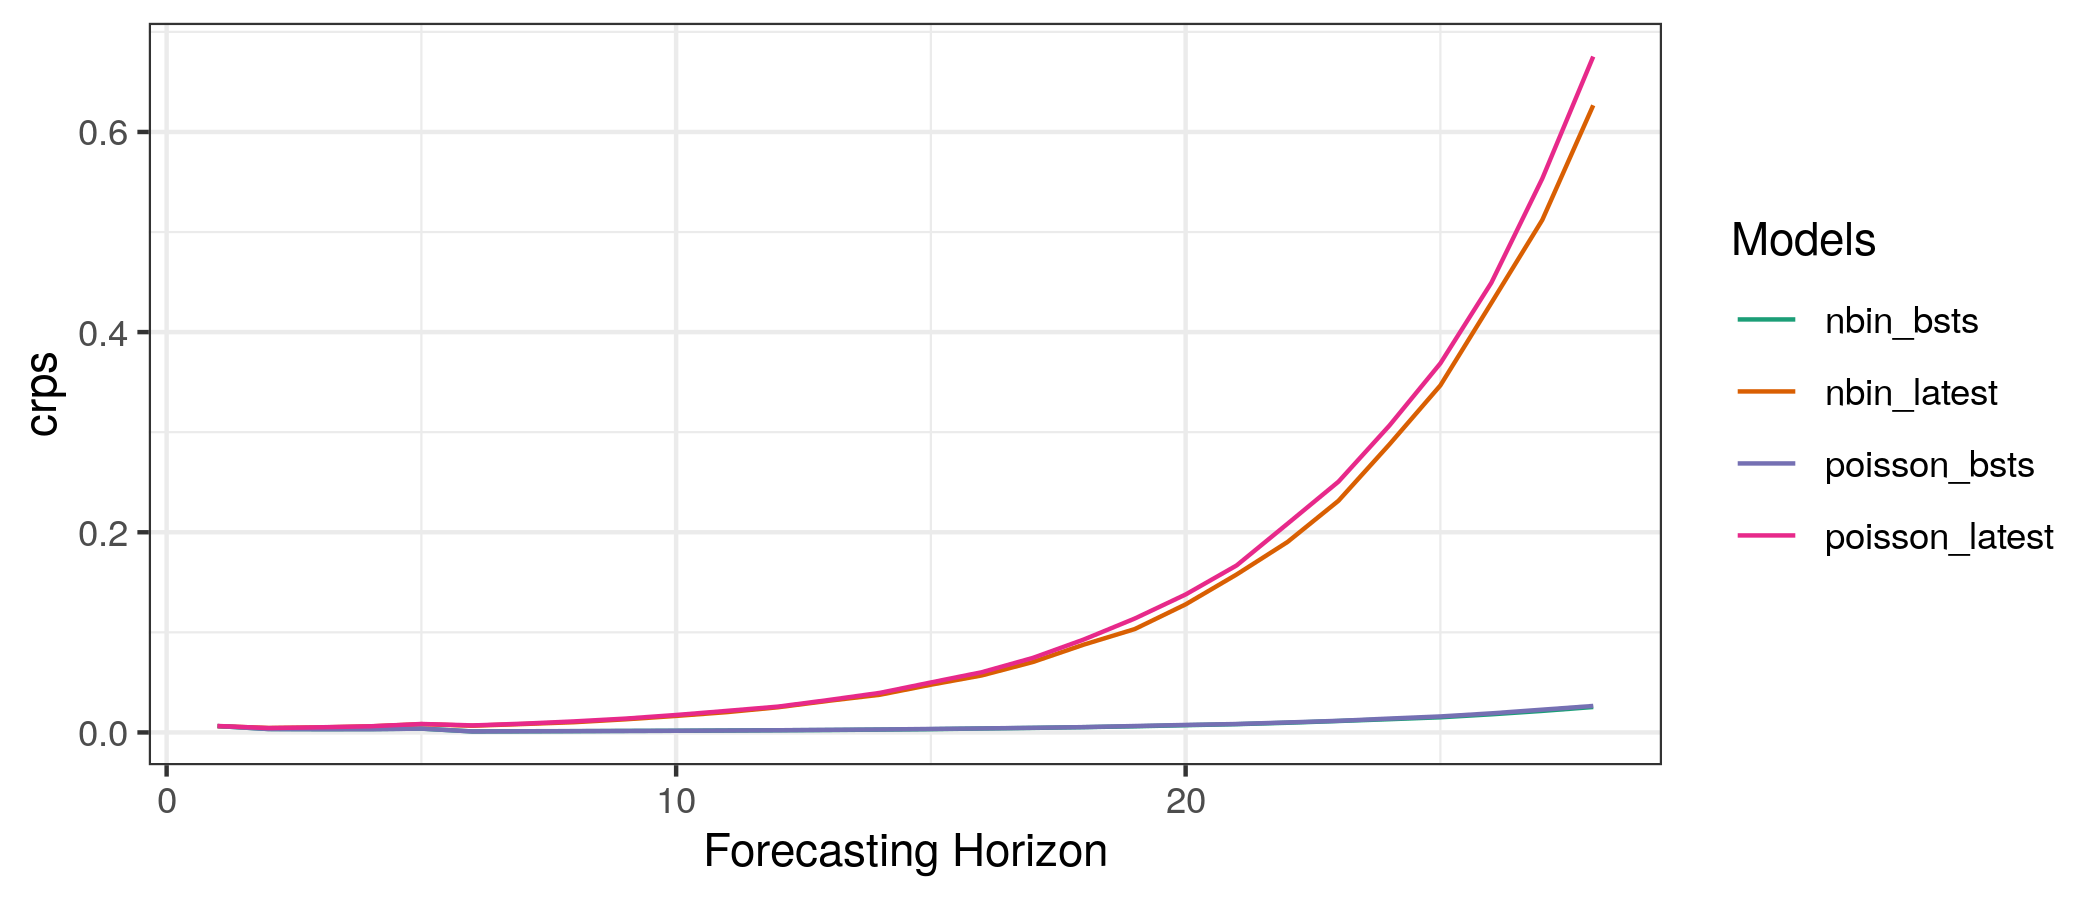
\includegraphics[width=\linewidth]{../output/Tchomia_crps.png}  
  \caption{Contineously Ranked Probability Score}
  \label{Tchomia_scores_1}
\end{subfigure}
\begin{subfigure}{0.5\textwidth}
  \centering
  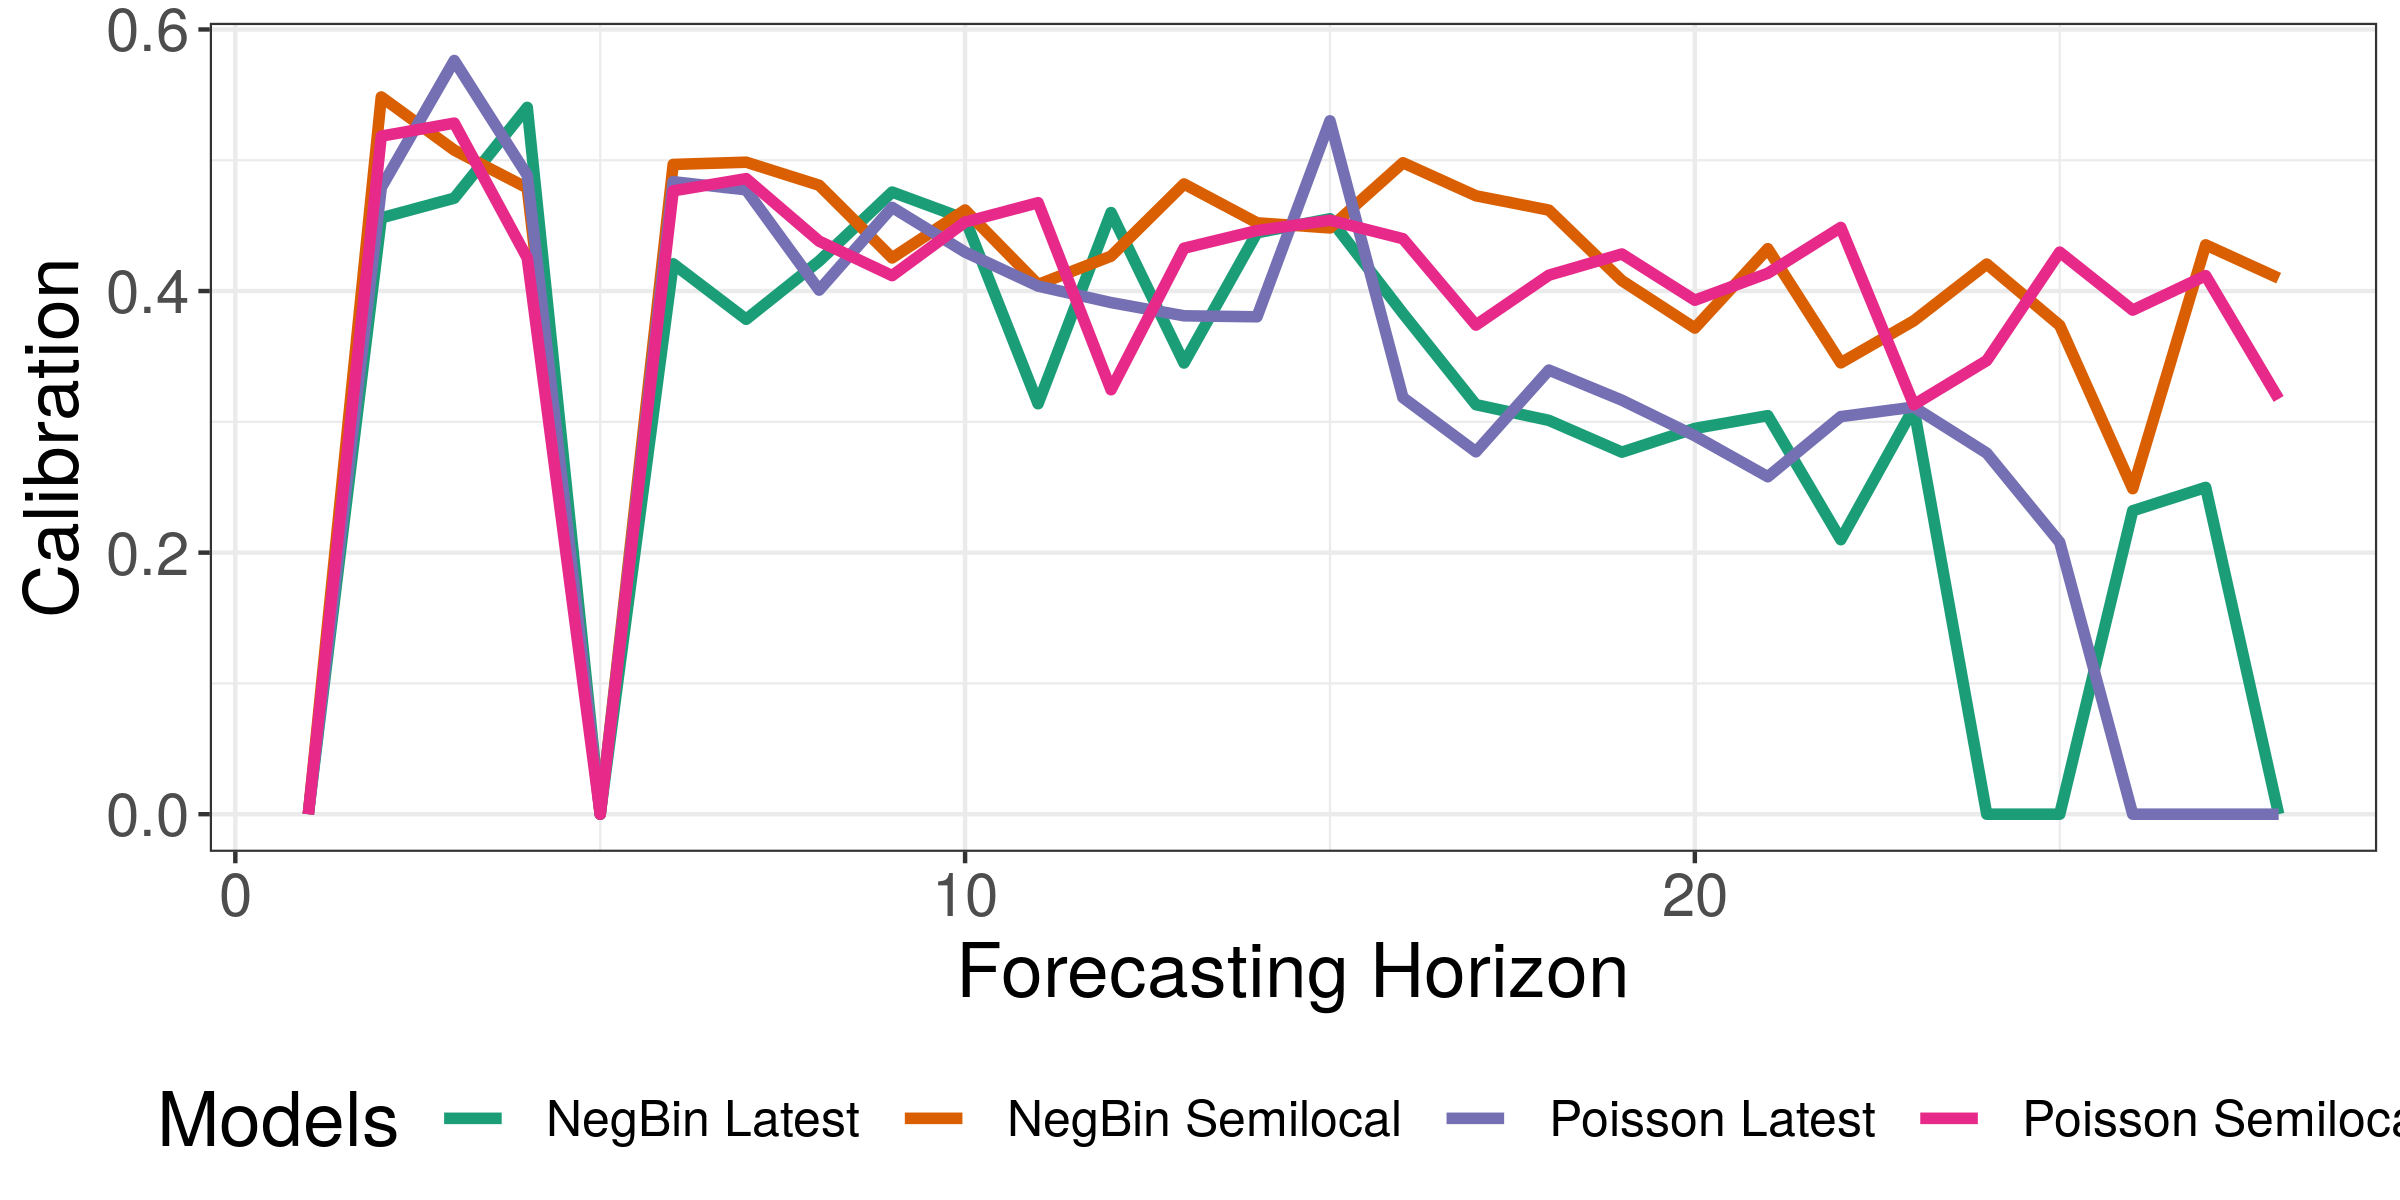
\includegraphics[width=\linewidth]{../output/Tchomia_calibration.png}  
  \caption{Calibration p-value}
  \label{Tchomia_scores_2}
\end{subfigure}

\begin{subfigure}{0.5\textwidth}
  \centering
  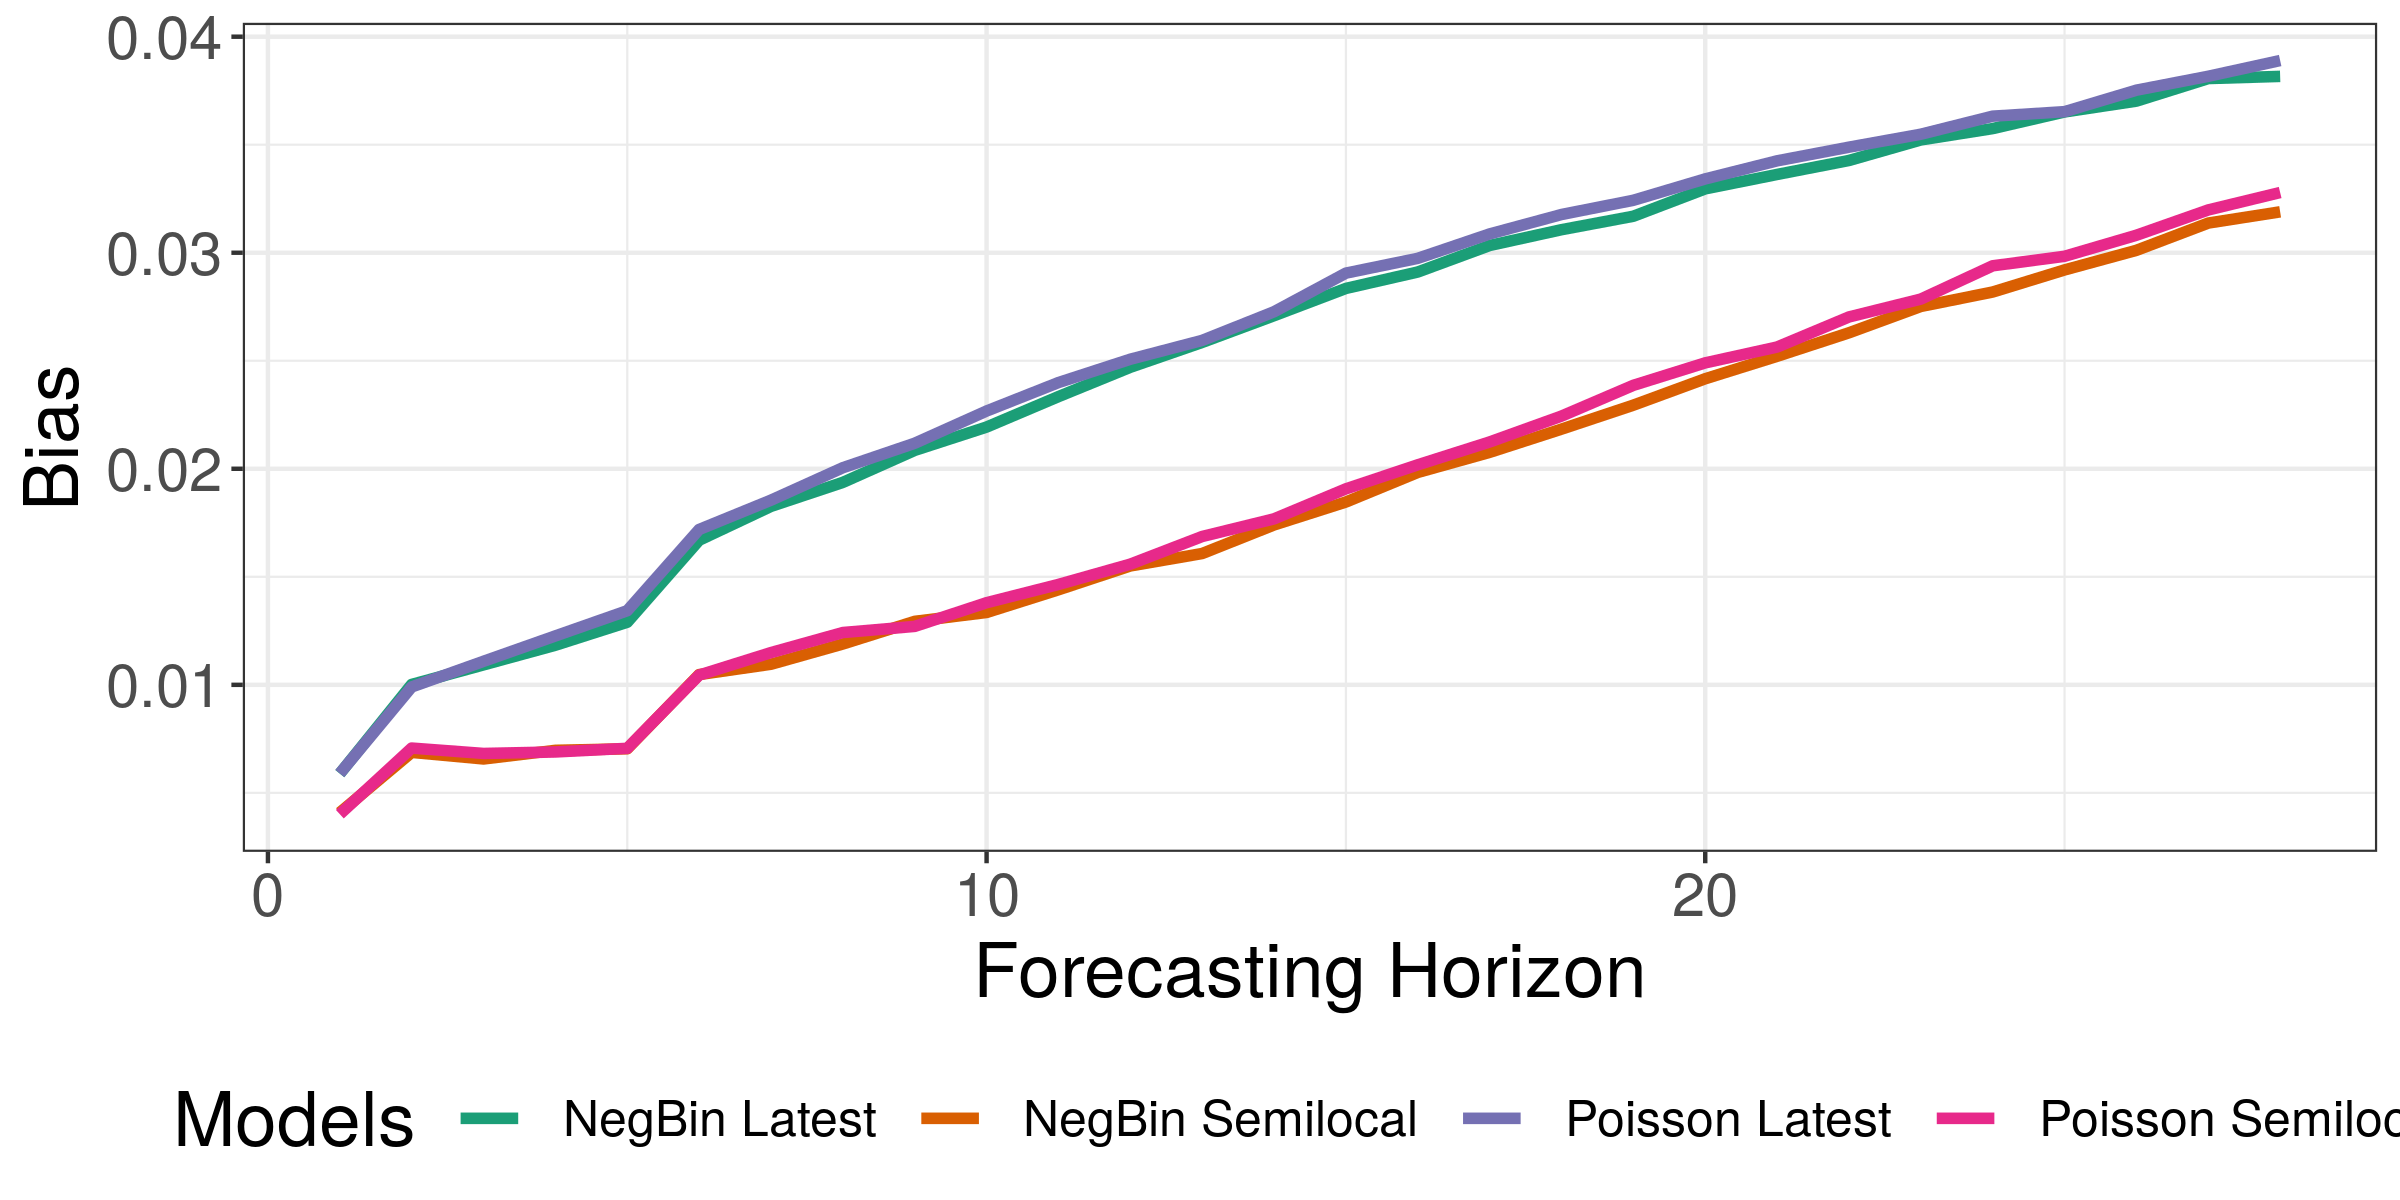
\includegraphics[width=\linewidth]{../output/Tchomia_bias.png}  
  \caption{Bias}
  \label{fig:Tchomia_scores_3}
\end{subfigure}
\begin{subfigure}{0.5\textwidth}
  \centering
  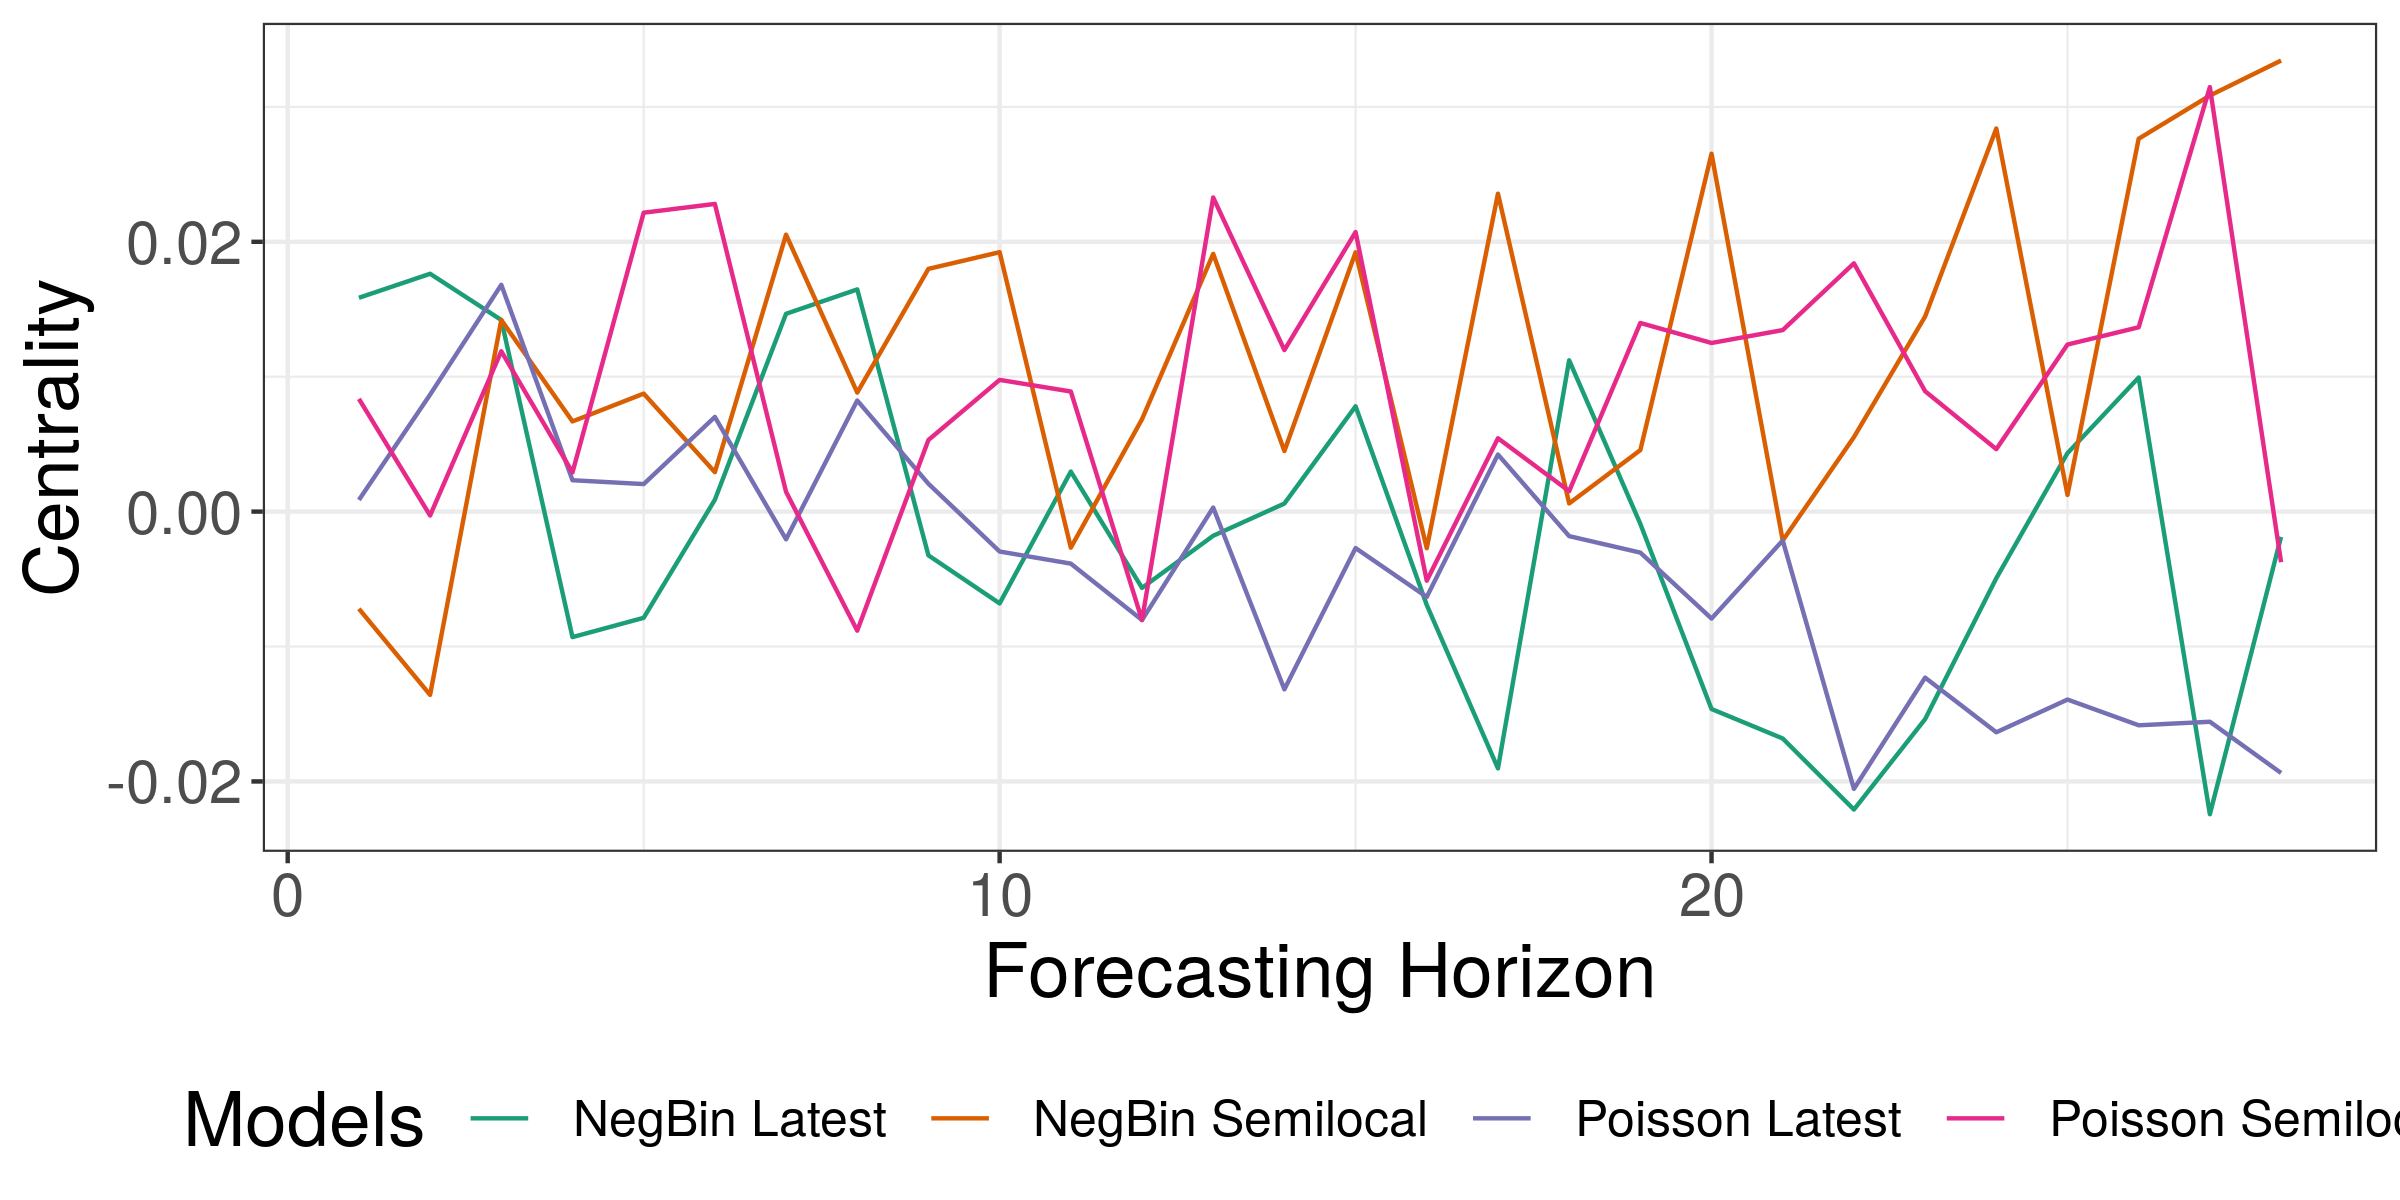
\includegraphics[width=\linewidth]{../output/Tchomia_centrality.png}  
  \caption{Centrality of PIT values}
  \label{fig:Tchomia_scores_4}
\end{subfigure}
  \caption{Scores for Tchomia as a function of the forecasting horizon.}

  \label{fig:nat_scores}
\end{figure}



\end{document}
